\documentclass[a4paper,fleqn,oneside,12pt]{report}

%%%%%%%%%%%%%%%%%%%%

\usepackage[]{geometry}
\usepackage[utf8]{inputenc}
\usepackage[UKenglish]{babel}
\usepackage[UKenglish]{isodate}
\usepackage{amsmath}
\usepackage{amsfonts}
\usepackage{amssymb}
\usepackage{amsthm}
\usepackage{graphicx}
\usepackage{chngpage}
\usepackage{calc}
\PassOptionsToPackage{hyphens}{url}
\usepackage{hyperref}
\usepackage[nameinlink]{cleveref}
\usepackage{fancyhdr}
\usepackage{titletoc}
\usepackage[explicit]{titlesec}
\usepackage{natbib}
\usepackage[dvipsnames]{xcolor}
\usepackage[sc]{mathpazo}
\linespread{1.05}
\usepackage[T1]{fontenc}
\usepackage{minted}
\usepackage{ragged2e}
\usepackage{adjustbox}
\usepackage{pifont}
\usepackage{tabularx}
\usepackage[justification=centering]{caption}

\newcommand{\cmark}{\ding{51}}
\newcommand{\xmark}{\ding{55}}
\newcommand{\W}{$\mathcal{W}$}
\newcommand{\M}{$\mathcal{M}$}
\newcommand{\comment}[1]{}

\hypersetup{
	colorlinks=true,
	linkcolor=black,
	urlcolor=black,
	citecolor=black
}

\definecolor{lightgrey}{rgb}{0.95,0.95,0.95}
\setminted{bgcolor=lightgrey}
\setmintedinline{bgcolor=lightgrey,escapeinside=||,mathescape=true}

\let\parencite\citep

\setlength{\parindent}{0mm}
\setlength{\parskip}{\medskipamount}
\renewcommand\baselinestretch{1.2}

\cleanlookdateon

\makeatletter
\newcommand{\@assignment}[0]{Assignment}
\newcommand{\assignment}[1]{\renewcommand{\@assignment}{#1}}
\newcommand{\@shorttitle}[0]{}
\newcommand{\shorttitle}[1]{\renewcommand{\@shorttitle}{#1}}
\newcommand{\@supervisor}[0]{}
\newcommand{\supervisor}[1]{\renewcommand{\@supervisor}{#1}}
\newcommand{\@yearofstudy}[0]{}
\newcommand{\yearofstudy}[1]{\renewcommand{\@yearofstudy}{#1}}
\makeatletter

%%%%%%%%%%%%%%%%%%%%%%%%%%%%%%%%%%%%%%%%%%%%%%%%%%%%%%%%%%%%%%%%%%%%%%%%%%%%%%%
%% Project-specific configuration
%%%%%%%%%%%%%%%%%%%%%%%%%%%%%%%%%%%%%%%%%%%%%%%%%%%%%%%%%%%%%%%%%%%%%%%%%%%%%%%

\author{Adam Jones}
\title{Interactive Tool for Teaching Hindley-Milner Type Inference through Visualisation}
\shorttitle{Interactive Tool for Teaching HM Type Inference through Visualisation}
\supervisor{Michael Gale}
\yearofstudy{3\textsuperscript{rd}}

%%%%%%%%%%%%%%%%%%%%%%%%%%%%%%%%%%%%%%%%%%%%%%%%%%%%%%%%%%%%%%%%%%%%%%%%%%%%%%%

\pagestyle{plain}
\renewcommand{\headrulewidth}{0.0pt}

\makeatletter
\fancypagestyle{plain}{
	\fancyhf{}
	%\fancyhead[LE]{\thepage}
	%\fancyhead[RE]{\textit{\@author}}
	\fancyhead[RO]{\thepage}
	\fancyhead[LO]{\textit{\@shorttitle}}
}
\makeatother

%%%%%%%%%%%%%%%%%%%%

\begin{document}

\makeatletter
\begin{titlepage}

	\textbf{\Huge Interactive Tool for Teaching\\Hindley-Milner Type Inference\\through Visualisation} \\[1.5cm]
    \Large \textbf{\@author} \\
    Department of Computer Science \\
    University of Warwick \\

	Supervised by \@supervisor \\
	Year of Study: \@yearofstudy \\

    \vfill

    \today

    \begin{adjustwidth}{-\oddsidemargin-1in}{-\rightmargin}
        \centering
        
\includegraphics[width=\paperwidth]{./line.png}
    \end{adjustwidth}

    \vspace*{-3.5cm}

\end{titlepage}
\makeatother

\pagestyle{plain}

\begin{abstract}
  Type inference is a process by which types in a program may be determined automatically by a compiler, without the need for explicit type annotations. Understanding of type inference helps programmers debug type errors and better understand type systems, however there are few accessible teaching resources available. We design and implement an interactive type inference teaching tool for a Hindley-Milner based expression language, which visualises and explains the steps taken by the common type inference algorithms \W, \W' and \M. User testing with undergraduate students shows the tool improves students' test scores on type and type inference (p < 0.001), and general feedback from users is positive. Analytics data provides evidence that the tool's output aids understanding and allows users to debug type errors.
\end{abstract}

\tableofcontents

\chapter{Introduction}\label{id:h.6k9gcmunzldy}

Types are common features of many programming languages. Generally, types are bounds on program constructs (such as variables, expressions and functions) that limit what valid values they may take and how they should be interpreted within the program, however different languages use types differently. Most type systems include primitive data types such as integers, booleans and characters as well as composite types such functions from one type to another and lists of a type.

Type checking is the process by which a language's compiler or interpreter validates that a program obeys the rules of the language's type system. When a violation is detected, such as providing a boolean to a function accepting an integer, a type error is raised.

Type checking is primarily used to catch bugs in program code, preventing unexpected behaviour. A simple example of this is function application: functions’ types specify how they can be called which ensure some pre-conditions are met, such as the arguments being of an expected type. This allows function implementers to safely assume the data is of that type, and prevents function users calling the function with invalid arguments.

Type checking can happen either at compile time (static type checking) or runtime (dynamic type checking).

Compile-time type checking prevents type errors from occurring at runtime. This is particularly useful when code paths may not be well tested or frequently used, as runtime type checking only surfaces type errors when the problematic code is executed. Additionally, knowing types at compile-time allows for better tooling that improves developer productivity. For example, IDEs may use type information to suggest and perform automated refactorings \citep{ref1}, automatically generate documentation \citep{ref2} and autocomplete statements \citep{ref3}.

Compile-time type checking requires the program code to have enough information to validate its type safety. This may be in the form of type annotations or typed variable and function declarations. However, specifying types manually can be time-consuming and potentially difficult as it is additional work for the programmer, and large composite types can be especially difficult to determine and tedious to repeatedly write.

A type inference algorithm for a programming language's type system can determine types automatically, which improves productivity by allowing programmers to get the best of types without having to explicitly specify them. Because of this, type inference is used in many popular programming languages with expressive type systems including Haskell, Rust and TypeScript.

Understanding type inference would help computer scientists write cleaner code and debug type errors. However, few universities have core modules on type systems (although they may be touched on in programming curriculums) and there are limited easy-to-understand teaching resources on type inference. Therefore, many computer science graduates will be missing a useful understanding of how type inference actually works.

The goal of this project is to develop a system to visualise the type inference process, to ultimately improve undergraduate students’ knowledge about it.

To achieve this, we create a teaching resource that explains how type inference algorithms work for functional languages based on the Hindley-Milner type system. An interactive web application allows students to enter custom expressions and view the results of a type inference algorithm, along with step-by-step explanations of how the algorithm determined that result. This is particularly useful in the context of modules teaching functional languages such as Haskell which perform similar type inference.

\section{Related work}\label{id:h.2mwaav7jkal4}

There have been previous attempts to build visualisation and teaching tools related to type systems.

One example is TypeTool by \cite{ref4}, which visualises type inference through a web application. Users enter an expression in a custom expression language, submit a request to a server and are redirected to a page displaying an initial syntax tree, a final syntax tree and an overall substitution. Allowing users to enter their own expressions allows students to explore how the system works under different cases to gain an intuitive understanding of the concepts.

{\centering \begin{figure}[h!]
  \centering
  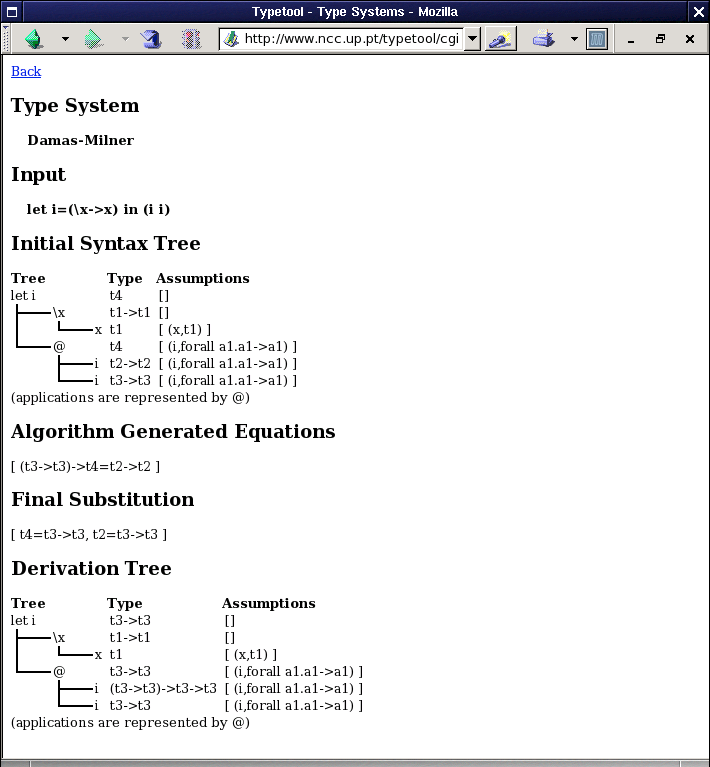
\includegraphics[width=0.75\linewidth]{images/image29.png}
  \caption{Screenshot of results from TypeTool, from their paper}
\end{figure} \par}

TypeTool's authors found in teaching the University of Porto's functional programming course that the tool was ``especially useful for students, because it helps to understand the type systems of the most common typed functional languages'' and that ``[presenting] the basis of type inference technology [...] significantly improved the way students deal with type errors because they understand the type system.''

However, TypeTool's parsing and type inference is done server-side so there is a delay between the user entering an expression and seeing the result. While short, a delay reduces the ease-of-use and may discourage users from trying many different expressions. Both delayed feedback and the lack of step-by-step explanations reduce learning quality \citep{ref5}, particularly in the area of rule learning. \cite{ref6} showed that immediate explanatory feedback is most effective at learning how to apply rules in computer programming.

It is unclear whether the tool supports incorrectly-typed expressions, which are important to explain as seeing when the type inference algorithm fails is critical to understanding why type errors are raised and how to go about resolving them.

TypeTool is also now inaccessible as the server hosting the application is no longer running and the source code has not been published.

Another tool in the area of visualising type systems was developed by \cite{ref7}. It is a visual functional programming system which shows types during function application for a subset of Standard ML, used to teach first year undergraduate students.

{\centering \begin{figure}[h!]
  \centering
  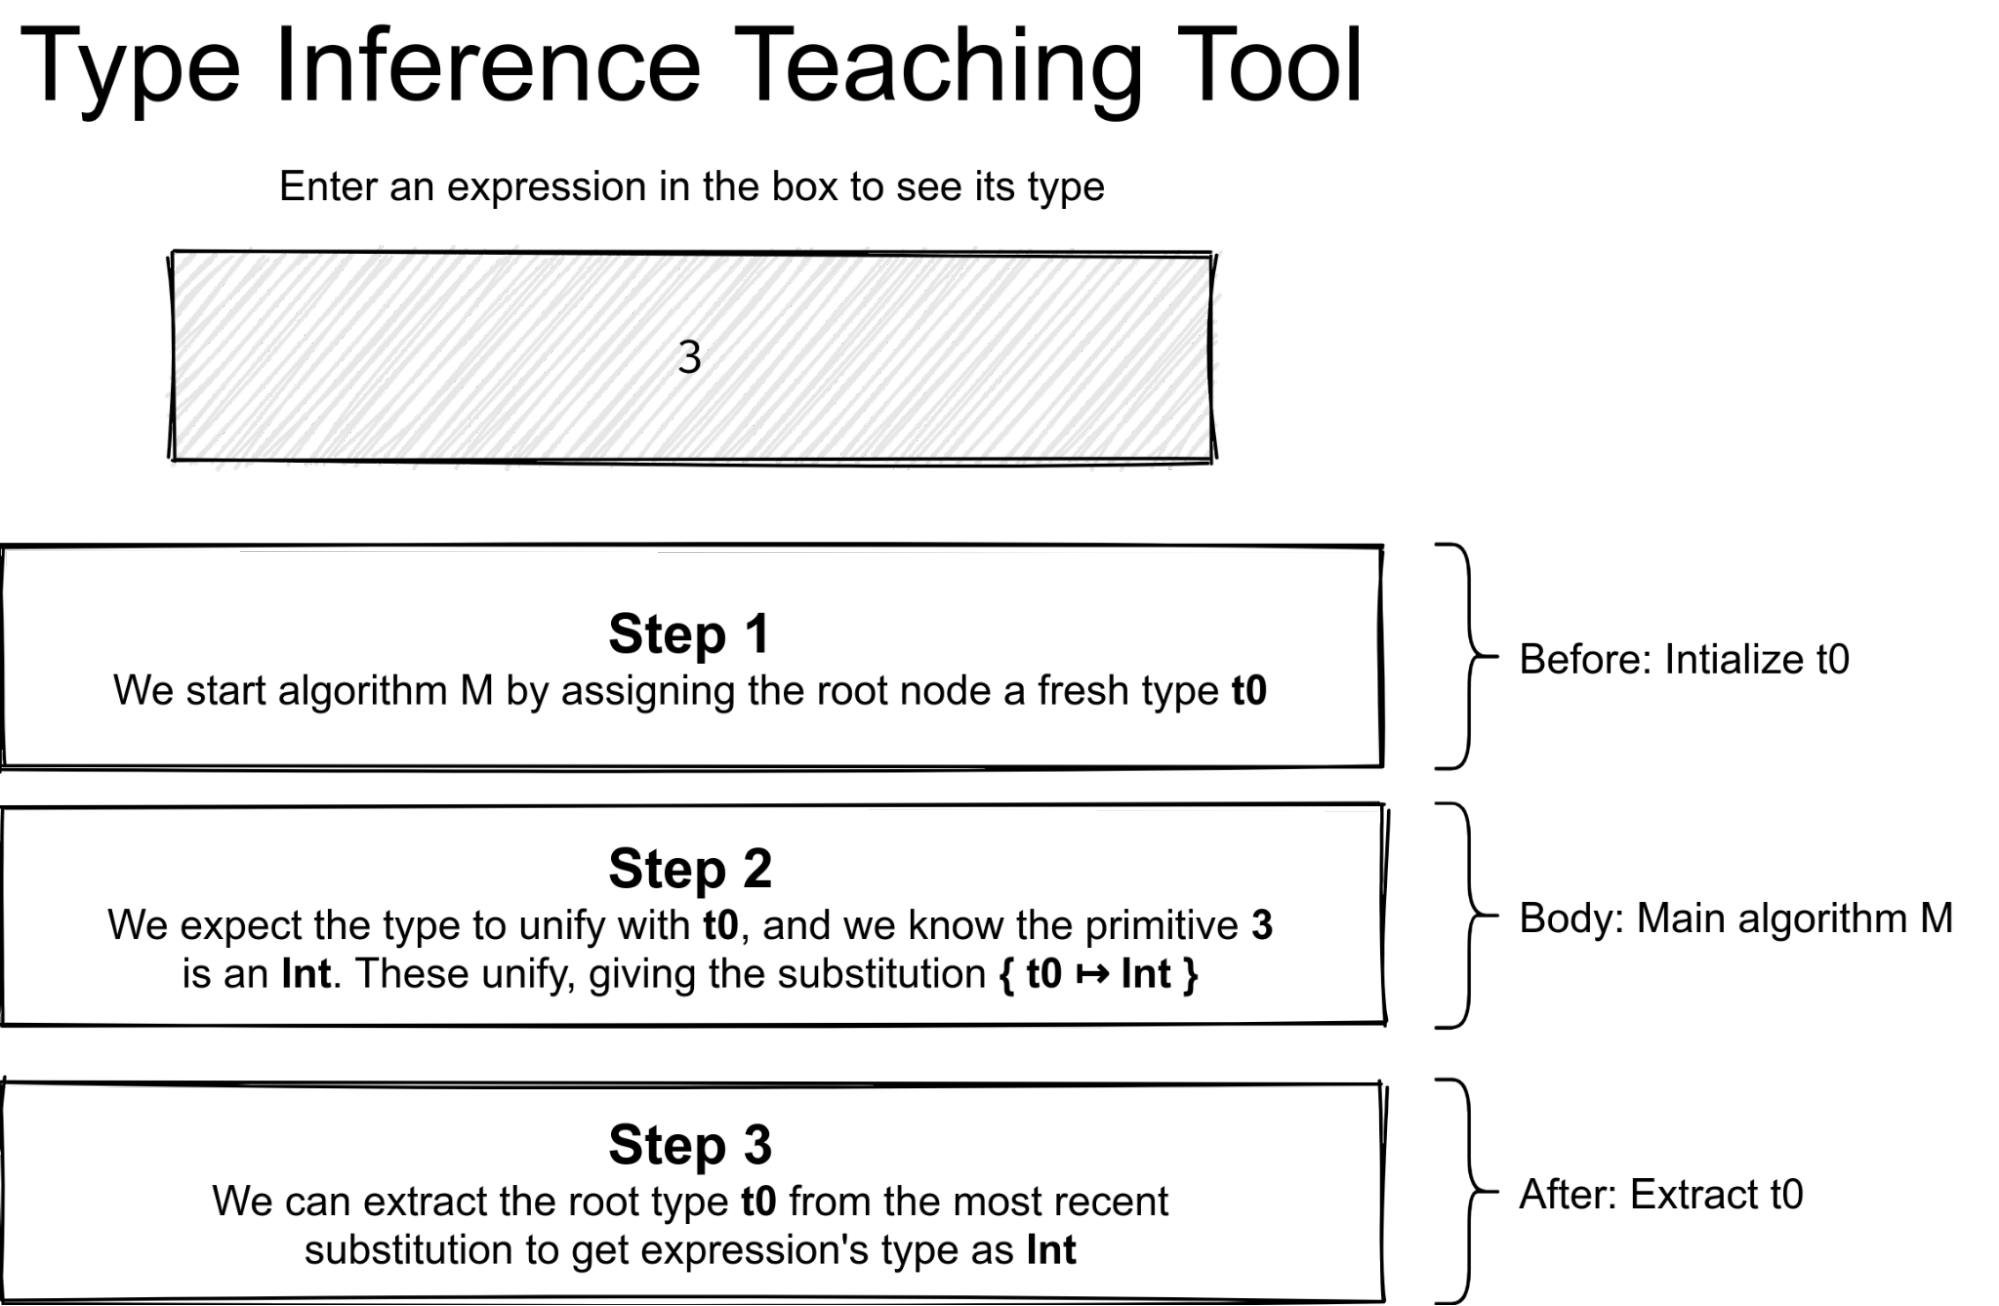
\includegraphics[width=0.75\linewidth]{images/image6.png}
  \caption{Screenshot of Yung and Michaelson's tool, from their paper}
\end{figure} \par}

However, this did not explicitly show the type inference process and as a desktop application rather than web app it is less accessible to lecturers and students. It also didn't support key functional language constructs such as function declarations and let bindings, and required significant explanation before using the tool to understand its output. Like TypeTool, this is no longer available to students.

NiMo \citep{ref8} is a graphical programming language related to functional data processing which allows users to reason about the flow of data through a program. The types of data and processes can be inspected in a software tool named NiMoToons, and type inference is performed over the network of components. However, larger expressions can become complicated and be difficult to interpret. While NiMo performs type inference internally it is not a key focus to the end-user, and as such does not explain its steps. Additionally, it is harder to relate back to more commonly used, textual functional languages like Haskell.

{\centering \begin{figure}[h!]
  \centering
  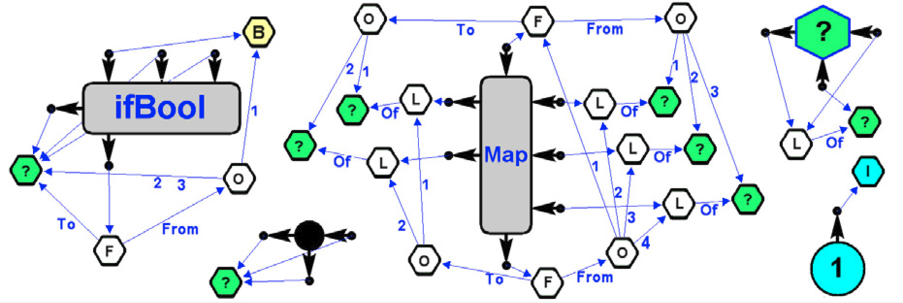
\includegraphics[width=\linewidth]{images/image25.png}
  \caption{The types of some variables in NiMo, from their paper}
\end{figure} \par}

\cite{ref9} implemented a successful teaching tool, named TILC, for visualising $\lambda$-calculus parse trees in order to help with teaching $\lambda$-calculus to undergraduate students. They noted that to develop an intuitive understanding, students would benefit from experimenting with $\lambda$-calculus and that “a tool that deals with all these aspects in a friendly and graphical manner incentivises [experimentation]”. TILC was beneficial for students, with the module organisers of `programming paradigms' at the Universitat de Girona having a ``good experience of using this tool in the course lectures and as a downloadable tool for students''. The authors suggested extending TILC to show types and type inference would have pedagogical value.

To summarise, types aid the construction of correct programs and type checking can detect issues in programs, either at compile-time or runtime. Type inference is a method often used alongside compile-time type checking to determine types in a program, an understanding of which could benefit computer scientists in writing and debugging programs. Some solutions exist which give students a better idea about types, however they either have significant limitations or do not explicitly cover type inference. In this report, we present an interactive web application for teaching type inference.

\chapter{Background}\label{id:h.ebjyqi73zdyo}

\section{\texorpdfstring{$\lambda$-}{Lambda }calculus}\label{id:h.odw4vku9eizz}

A $\lambda$-calculus is a representation of computation. The first $\lambda$-calculus set out by~\cite{ref10}, often viewed as the canonical $\lambda$-calculus, simply has variables, function abstraction and application.

For this project, we will consider a calculus with five constructs to build expressions from. As a formal grammar, expressions are:
$$\begin{array}{lcllll}
  \\
    \textrm{expression}\ e & ::= & c                       & \hspace{0.25cm} & \mathtt{con} & \textrm{(constant)}\\
                         & \vert & x                                       & & \mathtt{var} & \textrm{(variable)}\\
                         & \vert & e_1\ e_2                                & & \mathtt{app} & \textrm{(function application)}\\
                         & \vert & \lambda x.\ e                           & & \mathtt{abs} & \textrm{(function abstraction)} \\
                         & \vert & \mathtt{let}\ x = e_1\ \mathtt{in}\ e_2 & & \mathtt{let} & \textrm{(let statement)}\\
  \\
\end{array}$$

For example, consider the expression \mintinline{text}{(|$\lambda$|x. x) y}

It has variables \mintinline{text}{x} and \mintinline{text}{y}. Variables may be bound or free (unbound). Here \mintinline{text}{|x|} is bound as it is a parameter in the function abstraction, and \mintinline{text}{|y|} is free as there is nothing which binds it. This can be thought of in a similar way to how variables in most imperative programming languages have a scope where they are defined or undefined.

The function abstraction mentioned is the \mintinline{text}{|$\lambda$|x. x} part. This defines a function which given an argument (before the full stop) \mintinline{text}{x} simply returns (after the full stop) \mintinline{text}{x}, i.e. the identity function. A function to add three to an input might be written \mintinline{text}{|$\lambda$x. x + 3|} (although many of the most fundamental $\lambda$-calculi do not have such explicit notions of addition or numbers).

Functions may be returned by other functions, which enables them to have the appearance of taking multiple arguments. For example \mintinline{text}{|$\lambda$|x. (|$\lambda$|y. x)} can be viewed as a function which takes two arguments and returns the first one, even though really it is a function taking one argument which returns a function taking another argument for a result. Here explicit brackets have been given for clarity, but they aren’t necessary. Additionally, sometimes multiple arguments like this are written together, so \mintinline{text}{|$\lambda$|x. (|$\lambda$|y. x)}, \mintinline{text}{|$\lambda$|x. |$\lambda$|y. x} and \mintinline{text}{|$\lambda$|xy. x} all mean the same thing.

Finally, the function application is actually applying TODOthe function \mintinline{text}{|$\lambda$x. x|} to the argument \mintinline{text}{|y|}. In $\lambda$-calculus evaluation is performed via $\beta$-reductions. In our example this could be done by substituting the argument \mintinline{text}{|y|} for parameter \mintinline{text}{|x|} in the body of the function \mintinline{text}{|x|}, resulting in \mintinline{text}{|y|}.

This expression’s construction can be represented as an abstract syntax tree:

TODO: tree diagram of the expression

In addition to these three constructs, the let construct allows binding a value to a variable in an expression. For example \mintinline{text}{let x = 3 in x + x} binds \mintinline{text}{x} to the value \mintinline{text}{3} in \mintinline{text}{x + x}.

The con construct is added to represent literal constants, such as numbers or booleans like \mintinline{text}{3} and \mintinline{text}{True}.

$\lambda$-calculi have been extensively studied, often using formal inductive definitions. For example, the inductive definition for the set of free variables (\mintinline{text}{|var|}s not bound by function abstraction or let statements) is:

$$\begin{array}{lcl}
  \\
    FV(c)                                       & = & \varnothing\\
    FV(x)                                       & = & \{ x \}\\
    FV(e_1\ e_2)                                & = & FV(e_1) \cup FV(e_2)\\
    FV(\lambda x.\ e  )                         & = & FV(e) - \{ x \}\\
    FV(\mathtt{let}\ x = e_1\ \mathtt{in}\ e_2) & = & FV(e_2) - \{ x \}\\
  \\
\end{array}$$

Given these rules the set of free variables for any combination of these constructs can be determined. This can be demonstrated for our example expression \mintinline{text}{(|$\lambda$|x. x) y}, which is shown in a tree structure below. More generally this is an example of how an inductive definition can tell us something about the entire program which is how some type inference algorithms can be viewed.

TODO: tree diagram of the expression with the sets of free variables at each node.

Most real-world environments define a context which binds some variables by default to in-built values. For example Haskell’s GHC primitives and Prelude includes basic variables like \mintinline{text}{|[]|} (the empty list) and \mintinline{text}{|not|} (a function which inverts booleans). These can be considered bound at the top level and removed from the set of free variables there.

\section{The simply typed \texorpdfstring{$\lambda$-}{lambda }calculus}\label{id:h.w7vj0r89b86n}

Typed $\lambda$-calculi extend the system with the concept of types.

The simply typed $\lambda$-calculus is one of the simplest typed $\lambda$-calculi, and introduced by~\cite{ref11} is often viewed as the canonical typed $\lambda$-calculus. It has the \texttt{var}, \texttt{abs}, \texttt{app} and \texttt{con} constructs. Types in this system are either base types like $Int$s, $Bool$s and $Char$s (often represented in the literature by Greek letters $\alpha$, $\beta$, $\gamma$) or functions between other types such as $Int \rightarrow Bool$ or $Int \rightarrow (Bool \rightarrow Bool)$.

Compared to the untyped $\lambda$-calculus, the syntax of the simply typed $\lambda$-calculus adds type annotations to \texttt{var}, \texttt{abs} and \texttt{con} constructs, for example an expression may be written ($\lambda x: Int.\ odd^{Int \rightarrow Bool}\ x^{Int})\ 3^{Int}$. Often for simplicity the types of \texttt{var} and \texttt{con} subexpressions, those in superscript, are omitted.

\section{Hindley-Milner type system}\label{id:h.gsouq2axz3k}

Hindley-Milner (HM) is a typed $\lambda$-calculus which allows for the types of entire programs to be inferred with no type annotations required \citep{ref12,ref13}. It extends the simply typed $\lambda$-calculus by adding \texttt{let} bindings and a richer type system that includes \textit{type functions} and \textit{polymorphism}.

Like expressions, types can be considered to be built from \texttt{var\textsubscript{t}} variables and \texttt{app\textsubscript{t}} function applications. Type variables are either base types like $Bool$ and $Int$ or type functions. Type functions can be applied, taking types as parameters to construct composite types. Specifically, types made from \texttt{var\textsubscript{t}} and \texttt{app\textsubscript{t}} are known as \textit{monotypes}.
$$\begin{array}{lcllll}
  \\
    \textrm{monotype}\ \tau & ::= & t_n               & \hspace{0.25cm} & \mathtt{var_t} & \textrm{(type variable)}\\
                          & \vert & F\ \tau \dots \tau &                 & \mathtt{app_t} & \textrm{(type function application)}\\
  \\
\end{array}
$$
\vspace{-0.8cm}
$$
\textrm{where }F\textrm{ is a type function such as}\rightarrow\textrm{, }List\textrm{ or }Maybe.\\
$$
\vspace{0cm} % I don't know why this works but it does

For a type to be valid all functions must be fully applied, unlike expressions where the final expression may be a function. As with expressions, we can again assume a global context that binds variables like $Bool$ and $Int$. In Hindley’s original paper only $\rightarrow$ was considered as a type function (i.e. $F = \{ \rightarrow \}$), however here we explore several type functions that have been found useful in practice.

The type function we've already been using is $\rightarrow$ (the \textit{function} type function). It takes two types as arguments and represents a function from the first type to the second. A function from $Int$ to $Bool$ is represented by $(\rightarrow)\ Bool\ Int$ in prefix notation, although would more commonly be written infix as $Bool \rightarrow Int$.

The function type function ($\rightarrow$) should not be confused with a function type (e.g. $Bool \rightarrow Int$). An expression representing a function has a function type. That function type is the function type function applied to arguments. For example \mintinline{text}{|$\lambda$|x. x + 3} has a function type $Int \rightarrow Int$, which is the function type function $\rightarrow$ applied to arguments $Int$ and $Int$.

The list type function is also very common, which given one type argument represents a list of those types. A list of booleans might be written $List\ Bool$ or $[]\ Bool$ in prefix notation, although often the list type is represented by wrapping the type argument in square brackets instead, as in $[Bool]$. A string can be viewed as a list of characters, $[Char]$.

$Maybe$ is another type function commonly used in functional languages like Haskell. A $Maybe$ represents the optional presence of something, similar to Java’s \mintinline{java}{|Optional|} and C++’s \mintinline{c++}{|std::optional|}. Applied to a $Bool$ this may be written $Maybe\ Bool$, representing a wrapper around nothing or a boolean. In Java this would be represented with a generic as \mintinline{java}{|Optional<Boolean>|} and in C++ as \mintinline{c++}{|std::optional<bool>|}.

A similar common type function is $Either$, which takes two type arguments and represents a wrapper around either one of the types. For example, an either for a boolean or integer is written $Either\ Bool\ Int$. This is particularly helpful for functions that may fail, as they might return a result or error. For example, a function that returns a integer result or an error message may have the return type $Either\ Int\ [Char]$.

Finally, tuples represent a fixed-length sequence of elements of specific types. Tuple constructors are a set of type functions representing a cross product of their type arguments, named $(,)$ for 2-tuples, $(,,)$ for 3-tuples, $(,,,)$ for 4-tuples and so on for different element lengths. A 3-tuple holding a boolean, integer and integer can be written in prefix notation as $(,,)\ Bool\ Int\ Int$. However instead tuples usually borrow mathematical syntax with parentheses and commas and would be written as $(Bool,\ Int,\ Int)$.

$Bool$, $Maybe\ Int$, $Bool \rightarrow Int$, and $[(Bool,\ Int \rightarrow Maybe\ Bool)]$ are all examples of monotypes.

Adding zero or more for-all quantified type variables to monotypes forms polymorphic types or \textit{polytypes} (called principal type schemes by Hindley). This definition makes monotypes a special case of polytypes: monotypes are polytypes with zero for-all qualified type variables. We can therefore consider `type' in general to mean polytype (which include monotypes). Polytypes can be thought of as the \texttt{abs} equivalent for types. By convention, we represent free type variables with $t_0,\ t_1,\ t_2,\ \dots$ and use $a,\ b,\ c,\ \dots$ for for-all quantified type variables.

$$\begin{array}{lcllll}
  \\
    \textrm{polytype}\ \rho & ::= & \tau            & \hspace{0.25cm} & & \textrm{(monotype)}\\
                          & \vert & \forall a.\ \rho &                 & \mathtt{abs_t} & \textrm{(type function abstraction)}\\
  \\
\end{array}
$$

Polytypes allow for parametric polymorphism, where functions may accept different types as long as they meet certain constraints. For example the \mintinline{text}{length} function is polymorphic: it has the polytype $\forall a.\ [a] \rightarrow Int$, which accepts a list of any type and returns its length as an integer. \mintinline{text}{length} accepts multiple types such as $[Bool]$ and $[Int]$ as both of these meet the constraint of being a list.

Correctly inferring polymorphic types can be difficult, and in fact \cite{ref14} proved that doing so for System F, a type system similar to Hindley-Milner with fewer typing rule constraints, is undecidable. To prevent undecidability, HM avoids overusing polytypes, using only monotypes for \texttt{var}, \texttt{con}, \texttt{app} and \texttt{abs} expressions.

To allow for some polymorphism, the parameters of \texttt{let} expressions are polymorphic in the \texttt{let} body. The process by which the monomorphic parameter type is turned into a polymorphic one is known as \textit{generalisation}. The overall type of \texttt{let} expressions themselves are not generalised.

The difference can be seen by comparing similar \texttt{let} and \texttt{abs} expressions:
\begin{itemize}
  \item \mintinline{text}{let i = (|$\lambda$|x. x) in (i 3, i True)} type-checks, as i is generalised to the polytype $\forall a.\ a \rightarrow a$ within the body \mintinline{text}{(i 3, i True)} so can be applied to both an $Int$ and $Bool$.
  \item \mintinline{text}{(|$\lambda$|i. (i 3, i True)) (|$\lambda$|x. x)} does not type-check as the function abstraction \mintinline{text}{(|$\lambda$|x. x)} has the monotype $t_0 \rightarrow t_0$, and $t_0$ must take only one type in both tuple parts as it is not for-all qualified - it cannot be both an $Int$ and a $Bool$.
\end{itemize}

Hindley-Milner is the basis for the type system of Standard ML \citep{ref15}, which OCaml and F\# are related to, and was the basis of the type system in Haskell \citep{ref16}. It has influenced the development of Rust and Swift, and more generally type inference is present in many more languages including Java, JavaScript and C++.

Haskell's type system has since been extended with type-class constraints \citep{ref17}, functional dependencies \citep{ref18}, and generalised algebraic data types (GADTs) \citep{ref19}. Haskell’s inference engine was moved onto a new engine, OutsideIn(X), when GHC 7.2 was released November 2011 after \cite{ref20} proposed a solution to the issues with Hindley-Milner’s poor performance on large programs and difficulty inferring expressions without principal types that arise with type-class constraints and GADTs. This stopped Haskell automatically generalising variables bound by \texttt{let} expressions after \cite{ref21} argued that generalisation is hard in type inference engines other than HM and the feature was rarely used in practice, with the change only affecting 0.13\% lines of the GHC core libraries. This change does however take it further away from performing HM-like type inference.

Rust’s compiler, rustc, previously used a variant of HM for type inference. However, \cite{ref22} proposed a new scheme which was later implemented to simplify how the compiler reasoned about types. Similarly to Haskell’s move to OutsideIn(X), the new type inference reduces flexibility in some edge cases, although practically this is rare. Both rustc and Rust’s core libraries compiled under the new type inference scheme without changes. Later on, \cite{ref23} developed chalk, a library designed for use in rustc to help implement Rust’s generics. This library makes heavy use of unification, a key component of many HM type inference algorithms.

Apple's Swift language heavily uses type inference. It is implemented using a ``constraint-based type checker that is reminiscent of the classical Hindley-Milner type inference algorithm'' \citep{ref24}. Like other languages Swift extends HM with additional language features, including more expressive polymorphic types with additional constraints. HM is particularly suited to functional languages, so to adapt it to better suit Swift's procedural style, Swift limits type inference to individual statements rather than entire programs. This also improves performance and provides more specific error messages.

In addition to inferred types, most languages allow programmers to add more type information through explicit type annotations or casting. These features are particularly helpful where the programmer knows more than the inference algorithm about the limits on how a part of a program will be used.

Java allows casting and TypeScript has its \mintinline{text}{|as|} type assertion operator. These can be used sparingly (often in combination with \mintinline{text}{instanceof} and \mintinline{text}{typeof} operators respectively) as an escape hatch to work around the limitations of type inference algorithms. These statements may not be able to be type checked at compile-time so instead runtime checks are performed to maintain type safety.

Java allows casting an object to a subclass \citep{ref25}. Runtime checks are performed, which throw a \mintinline{text}{|ClassCastException|} in case the object is not actually an instance of the subclass.

\begin{minted}[breaklines]{java}
/* Dog and Cat extend Animal */

Animal c1 = new Dog();
Dog s1 = (Dog) c1; // okay

Animal c2 = new Cat();
Dog s2 = (Dog) c2; // throws ClassCastException at runtime
\end{minted}

TypeScript can cast compatible objects with its \mintinline{text}{as} operator. Alternatively, compile-time type checking may be overridden completely with a \mintinline{text}{@ts-ignore} comment. The following shows that some type-safe code is rejected by the TypeScript type checker, but has several possible workarounds.

\begin{minted}[breaklines]{typescript}
// has type "cs310" | 310
const a = Math.random() < 0.5 ? 'cs310' : 310;

// throws a type error, but b could have type "cs310cs310" | 620
const b = a + a;

// has type number | string
const c = a == 'cs310' ? a + a : a + a;

// has type any
const d = a as any + a;

// has type "cs310cs310" | 620
const e = a as any + a as 'cs310cs310' | 620

// has type "cs310cs310" | 620
/* @ts-ignore */
const f: 'cs310cs310' | 620 = a + a;
\end{minted}

TODO: (maybe?) Add section on TypeScript/Elm?
\underline{\href{https://aaltodoc.aalto.fi/bitstream/handle/123456789/42719/master\_Mikkonen\_Juuso\_2020.pdf}{https://aaltodoc.aalto.fi/bitstream/handle/123456789/42719/master\_Mikkonen\_Juuso\_2020.pdf}}
Talks about statically typed languages in JavaScript-land. Mentions things like TypeScript don’t use HM because JS has a lot of structural typing (i.e. if objects have the right properties it’s fine to call methods that depend on that interface) and subtyping.

While real-world languages don't work exactly like HM, for the purposes of the teaching tool HM gives a good representation of how type inference works to students. HM avoids being too complex to understand, and is still related to how languages commonly used in practice perform type inference.

\section{Hindley-Milner type inference}\label{id:h.admfqf7bhkct}

Various type inference algorithms are available for the Hindley-Milner type system. These include Algorithm \W\ by \cite{ref13} and Algorithm \M\ by \cite{ref27}. \W\ takes a bottom-up approach, attempting to infer the types of subexpressions up the abstract syntax tree, while \M\ takes a top-down approach, inferring types down the tree. Algorithm \W' is a minor extension of \W\ by \cite{ref28} which can improve the quality of type errors raised.

\subsection{Substitutions}

Substitutions are a key concept from logic used by all three algorithms. These are maps from variables to terms. When applied to a value, the variables are substituted by their corresponding terms. In type inference, the variables are type variables, the terms are monotypes and values are types.

Substitutions are represented with curly braces, with each entry separated by a comma and the variables and terms separated with an arrow. For example, the susbtitution $\{ t_0 \mapsto t_1,\ t_2 \mapsto (Int, Bool) \}$ would replace $t_0$ with $t_1$, and replace $t_2$ with $(Int, Bool)$. Applying it to the type $t_0 \rightarrow t_1 \rightarrow t_2$ would result in $t_1 \rightarrow t_1 \rightarrow (Int, Bool)$.

When applying substitutions replacements are performed simultaneously, so each variable in the type may be mapped at most once. For example the substitution $S = \{ t_0 \mapsto t_1,\ t_1 \mapsto t_2 \}$ applied once to the type $t_0$, as $S(t_0)$ results in $t_1$, not $t_2$. Applying the substitution twice, $S(S(t_0))$ results in $t_2$.

Any number of substitutions may be applied to a type. For example, given two substitutions $S_1 = \{ t_0 \mapsto t_2,\ t_1 \mapsto t_3 \}$ and $S_2 = \{ t_0 \mapsto t_1 \}$, we may apply both to a type $t_0$. Note that substitutions are not commutative, $S_1(S_2(t_0)) = t_3$ while $S_2(S_1(t_0)) = t_2$.

Substitutions may be combined to have the same effect as applying them in order to an type $\rho$. For example, with substitutions $S_1 = \{ t0 \mapsto t2,\ t1 \mapsto t3 \}$ and $S_2 = \{ t0 \mapsto t1 \}$ again, we have:
$$\mathit{combine}(S_1,\ S_2)(\rho) = S_1(S_2(\rho)) = \{ t0 \mapsto t3,\ t1 \mapsto t3 \}(\rho)$$

As application is not commutative, the order substitutions are combined in matters, i.e. $\mathit{combine}(S_1,\ S_2)$ does not necessarily equal $\mathit{combine}(S_2,\ S_1)$. Combining substitutions is however associative, as:
\begin{align*}
  \mathit{combine}(S_1,\ \mathit{combine}(S_2,\ S_3))(\rho) & = S_1(S_2(S_3(\rho)))\\& = \mathit{combine}(\mathit{combine}(S_1,\ S_2),\ S_3)(\rho)
\end{align*}

\subsection{Unification}

A substitution is said to unify two values if when applied to both it results in equal values. For example, $\{ t_0 \mapsto Int,\ t_1 \mapsto Bool \}$ unifies $(t_0,\ Bool)$ and $(Int,\ t_1)$, as it is applied to either expression the result is $(Int,\ Bool)$.

Unification is the process of finding unifying substitutions given two values, or reporting no such substitution exists. \cite{ref29} presents a simple algorithm for unification, and both \cite{ref30} and \cite{ref31} set out linear time unification algorithms.

In the type inference algorithms \W, \W’ and \M, unification is applied to pairs of monotypes. This results in substitutions which effectively combine the various type constraints giving us a final type.

For example, take an expression satisfying two type constraints: it matches the monotype $[Bool] \rightarrow t_0$ and it matches with the monotype $[t_1] \rightarrow t_1$. These constraints might arise in evaluating the type of \mintinline{text}{head [True]}. The first constraint is from knowing \mintinline{text}{[True]} is a $[Bool]$ so the function should accept a $[Bool]$. The second constraint is based on the known definition of \mintinline{text}{head} in the global context. Unification can find the unifying substitution $\{ t_0 \mapsto Bool, t_1 \mapsto Bool \}$, giving the overall type $[Bool] \rightarrow Bool$. We can then see the resultant type of \mintinline{text}{head [True]} is $Bool$.

If unification is not possible, the type constraints must be incompatible and so a type error is raised. For example, there is no unifying substitution for $Int \rightarrow t_0$ and $Bool \rightarrow t_1$ as one is a function accepting an $Int$ and the other accepts a $Bool$.

For practical purposes, type inference algorithms require unifying substitutions to be finite as infinite types are difficult to represent and reason about. For example \mintinline{text}{x} in \mintinline{text}{|$\lambda$|x. x x} needs to be a function that accepts itself. Initially assuming \mintinline{text}{x} has type $t_0 \rightarrow t_1$ and knowing it should accept itself, it also has type $(t_0 \rightarrow t_1) \rightarrow t_1$. It also must accept that, so has type $((t_0 \rightarrow t_1) \rightarrow t_1) \rightarrow t_1$, $(((t_0 \rightarrow t_1) \rightarrow t_1) \rightarrow t_1) \rightarrow t_1$, and so on. This is an infinite type and is not allowed by HM. Note that this does not exclude functions from HM which do accept themselves, such as the identity function \mintinline{text}{id} with its type $\forall a.\ a \rightarrow a$, as long as they have finite types.

Detecting infinite types in unification is done by checking whether the types are not equal and one of the types occurs in another. This is known as the \textit{occurs check}. In the previous example \mintinline{text}{|$\lambda$|x. x x} we might try to unify $t_0 \rightarrow t_1$ with $t_0$. $t_0$ occurs in $t_0 \rightarrow t_1$ so there is no finite unifying substitution (an infinite unifying substitution is $\{ t_0 \mapsto ((((t_0 \rightarrow t_1) \rightarrow t_1) \rightarrow \textrm{infinite }t_1\textrm{s} \dots) \rightarrow t_1) \}$). The occurs check failing necessarily means we have an infinite type: the type contains itself.

\subsection{Contexts}

Inferring types is done in a typing context. Languages often have a global context with built-in functions and their types pre-defined, such as Haskell’s Prelude and JavaScript’s global objects.

Typing contexts can be seen as maps from variable names to their corresponding types, and are represented with the symbol $\Gamma$. A simple context may be written $\Gamma = \{ \mathtt{not} : Bool \rightarrow Bool,\ \mathtt{odd} : Int \rightarrow Bool,\ \mathtt{id} : \forall a.\ a \rightarrow a \}$.

Constructs that bind variables like \texttt{let} and \texttt{abs} add entries to a local context for these additional bindings, used in the construct bodies. For example, in \mintinline{text}{let x = 3 in odd x} the binding $\mathtt{x} : Int$ may be added to the context used to perform type inference on the body subexpression \mintinline{text}{odd x}. Similarly in \mintinline{text}{|$\lambda$|x. not x} the binding $\mathtt{x} : t_0$ may be added to the context for inferring the type of the function body \mintinline{text}{not x}. Adding a binding is represented by a $+$, so given $\Gamma = \{ \mathtt{x} : Bool \}$ then $\Gamma + \mathtt{y} : Int$ is $\{ \mathtt{x} : Bool,\ \mathtt{y} : Int \}$.

Applying a substitution to a context is to apply the substitution to every type in the context, or effectively every `value' in the key-value map. To illustrate with an example, applying the substitution $S = \{ t_0 \mapsto t_1,\ t_2 \mapsto Int \}$ to the context $\Gamma = \{ \mathtt{x} : t_0,\ \mathtt{y} : t_1,\ \mathtt{z} : t_2 \}$, results in a new context $S(\Gamma) = \{ \mathtt{x} : t_1,\ \mathtt{y} : t_1,\ \mathtt{z} : Int \}$.

\subsection{Instantiation and generalisation}

Some types are considered more general than others. A type $\rho_a$ is more general than a type $\rho_b$ if there exists a substitution from $\rho_a$ to $\rho_b$ whose variables are for-all quantified in $\rho_a$. This is denoted by $\sqsubseteq$, for example $\forall a.\ a \rightarrow a$ is more general than $Int \rightarrow Int$ by the substitution $\{ a \mapsto Int \}$, written $\forall a.\ a \rightarrow a \sqsubseteq Int \rightarrow Int$.

Substitutions may (and often do) substitute quantified type variables with free type variables like $t_0$ and $t_1$, rather than concrete types like $Int$ and $Bool$. For example:
\begin{align*}
\hspace{0.75cm}\forall a & \forall b.\ (a \rightarrow b) \rightarrow [a] \rightarrow [b]
\\& \sqsubseteq \forall a.\ (a \rightarrow Bool) \rightarrow [a] \rightarrow [Bool] &\textrm{by}\ \{ b \mapsto Bool \}
\\&\sqsubseteq (t_0 \rightarrow Bool) \rightarrow [t_0] \rightarrow [Bool] &\textrm{by}\ \{ a \mapsto t_0 \}
\end{align*}

For any type $\rho \sqsubseteq \rho$, as the substitution may be empty. A type is strictly less general ($\sqsubset$) than another if and only if the substitution is non-empty. This means a strictly less general type must have at least one fewer quantified variable, because one for-all quantified variable must have been substituted away.

TODO: (maybe) partial order diagram of some of $\forall a \forall b.\ (a \rightarrow b) \rightarrow [a] \rightarrow [b]$’s partial and full instantiations.

An expression with a type $\rho_a$ more general than another type $\rho_b$ can be considered to have the less general type $\rho_b$. This means if an expression with type $\rho_b$ is needed, providing an expression with type $\rho_a$ will type-check if and only if $\rho_a \sqsubseteq \rho_b$. The process of giving an expression a less general type is known as \textit{instantiation}. For example, the type of \mintinline{text}{id}, $\forall a.\ a \rightarrow a$, can be instantiated as all of $Int \rightarrow Int$, $Bool \rightarrow Bool$, $t_0 \rightarrow t_0$ or even $([t_0] \rightarrow (Int,\ Bool)) \rightarrow ([t_0] \rightarrow (Int,\ Bool))$.

The `opposite' of instantiation is generalisation, where an expression with a certain type can be considered to have a more general type, adding a for-all quantification to a variable. This is allowed where the type variable is not free in any of the types in the context. Not being free in the context means the type variable does not appear unbound anywhere except in the type being generalised itself, so it does not have any other type constraints. Being free of any type constraints, it may be any type and therefore for-all quantified.

Given a type $t_0 \rightarrow t_1 \rightarrow t_2 \rightarrow t_3$ and a context $\{ \mathtt{x} : t_1,\ \mathtt{y} : [t_2] \rightarrow Int,\ \mathtt{z} : \forall t_3.\ t_3 \}$ we may generalise to $\forall t_0 \forall t_3.\ t_0 \rightarrow t_1 \rightarrow t_2 \rightarrow t_3$. $t_0$ is not in any of the types in the context, and $t_3$ is only found bound as a for-all quantified variable. Therefore both of these may be for-all quantified. Both $t_1$ and $t_2$ are free in the context, so may not be generalised. (Note we are disregarding our convention of using $a,\ b,\ c,\ \dots$ for for-all quantified variables here, to be strict to the typing rules. Renaming the type variables with $\alpha$-conversions could be done after generalisation to maintain the type variable naming conventions.) Given a context and type, the function $\mathit{generalise}$ returns the fully generalized type possible in that context.

\subsection{Typing rules}

Our key syntax rules plus instatitation and generalisation lead to nine typing rules. Many presentations of Hindley-Milner do not include literal constants in their syntax, or do not explicitly type them given their triviality. Here we give them for completeness.

$$
\begin{array}{ccl}
  \displaystyle\frac{}{\vdash c_{Int} : Int} & \hspace{0.25cm} & \mathtt{con_{Int}}\\ \\
  \displaystyle\frac{}{\vdash c_{Char} : Char} & & \mathtt{con_{Char}}\\ \\
  \displaystyle\frac{}{\vdash c_{Bool} : Bool} & & \mathtt{con_{Bool}}\\ \\
  \displaystyle\frac{x : \rho \in \Gamma}{\Gamma \vdash x : \rho} & & \mathtt{var}\\ \\
%\end{array}
%$$
%$$
%\begin{array}{ccl}
  \displaystyle\frac{\Gamma \vdash e_0 : \tau \rightarrow \tau' \quad\quad \Gamma \vdash e_1 : \tau }{\Gamma \vdash e_0\ e_1 : \tau'} & & \mathtt{app}\\ \\
  \displaystyle\frac{\Gamma,\ x : \tau\vdash e : \tau'}{\Gamma \vdash \lambda x.\ e : \tau \rightarrow \tau'} & & \mathtt{abs}\\ \\
  \displaystyle\frac{\Gamma \vdash e_0 : \rho \quad\quad \Gamma,\ x:\rho \vdash e_1 : \tau}{\Gamma \vdash \mathtt{let}\ x = e_0\ \mathtt{in}\ e_1 : \tau} & & \mathtt{let}\\ \\
  \displaystyle\frac{\Gamma \vdash e : \rho' \quad\quad \rho' \sqsubseteq \rho}{\Gamma \vdash e : \rho} & & \mathtt{instantiate}\\ \\
  \displaystyle\frac{\Gamma \vdash e : \rho \quad\quad a \notin \text{free}(\Gamma)}{\Gamma \vdash e : \forall a.\ \rho} & & \mathtt{generalise}\\ \\
\end{array}
$$

These typing rules can be used to deduce and prove the types of expressions. For example, the expression \mintinline{text}{|not True|} in a context $\Gamma = \{ \mathtt{not} : Bool \rightarrow Bool \}$:

$$
\begin{array}{lclc}
  \Gamma \vdash \mathtt{not} : Bool \rightarrow Bool & \hspace{0.25cm} & \textrm{by}\ \mathtt{var}        & \hspace{4cm} \\
  \vdash \mathtt{True} : Bool                        &                 & \textrm{by}\ \mathtt{con_{Bool}} & \\
  \Gamma \vdash \mathtt{not\ True} : Bool            &                 & \textrm{by}\ \mathtt{app}        & \\
\end{array}
$$

Despite this, the typing rules themselves aren't an algorithm as they do not specify an order to be applied in. While only one syntax rule can apply to a subexpression, it may be unclear when to apply instantiation and generalisation. Arbitrarily applying rules does not necessarily converge to a solution, as generalisation and instantiation can both continue infinitely. For example repeatedly applying instantiation and generalisation on \mintinline{text}{id} with $\Gamma = \{ \mathtt{id} : \forall a.\ a \rightarrow a \}$:

$$
\begin{array}{lclc}
  \Gamma \vdash \mathtt{id} : \forall a.\ a \rightarrow a & \hspace{0.25cm} & \textrm{by}\ \mathtt{var} & \\
  \Gamma \vdash \mathtt{id} : [t_0] \rightarrow [t_0] & & \textrm{by}\ \mathtt{instantiate}\ \textrm{with}\ \{ a \mapsto [t_0] \}& \\
  \Gamma \vdash \mathtt{id} : \forall b. [b] \rightarrow [b] & & \textrm{by}\ \mathtt{generalise} & \\
  \Gamma \vdash \mathtt{id} : [[t_1]] \rightarrow [[t_1]] & & \textrm{by}\ \mathtt{instantiate}\ \textrm{with}\ \{ b \mapsto [t_1] \} & \\
  \Gamma \vdash \mathtt{id} : \forall c. [[c]] \rightarrow [[c]] & & \textrm{by}\ \mathtt{generalise} & \\
  \Gamma \vdash \mathtt{id} : [[t_2]] \rightarrow [[t_2]] & & \textrm{by}\ \mathtt{instantiate}\ \textrm{with}\ \{ c \mapsto [t_2] \} & \\
  \dots & & & \\
\end{array}
$$

The type inference algorithms \W, \W’ and \M\ effectively are methods to select typing rules to determine a type for the expression, or detect the expression is incorrectly typed. While they don't apply the typing rules directly, they are close and their respective authors prove they give equivalent results and can be implemented directly.

The algorithms are applied to abstract syntax trees (ASTs), which represent expressions in a structured way. For example, an AST for the expression \mintinline{text}{let y = (|$\lambda$|x. (odd x)) 3 in not y} may be visualised as:

TODO: tree diagram of expression

The type inference algorithms are therefore tree traversal algorithms. They generally call themselves recursively on subtrees to process subexpressions, and then combine these results to determine a final type (the type of the root node).

\subsection{Algorithm \texorpdfstring{\W}{W}}

Algorithm \W\ is often seen as \textit{the} Hindley-Milner type inference algorithm. Given a context and an expression represented as an abstract syntax tree, it returns a substitution and a monotype.

The purpose of returning the type is obvious, but the substitution's purpose is less so. The substitution represents constraints on type variables that have arisen from performing type inference on the expression. For example, given a context $\{ \mathtt{f} : t_0, \mathtt{not} : Bool \rightarrow Bool \}$ and an expression \mintinline{text}{not (f 3)} we might return the type $Bool$ and the substitution $\{ t_0 \mapsto Int \rightarrow Bool \}$. This substitution is important because if \mintinline{text}{f} or the type variable $t_0$ are used elsewhere in the same expression we need to type-check those occurrences for consistency with this usage. In a wider expression such as \mintinline{text}{|[not (f 3), f True]|} the substitution from our first subexpression tells us type $t_0$ is $Int \rightarrow Bool$. When examining the application of the second \mintinline{text}{|f|}, we find its type from the context which is $t_0$, or equivalently now $Int \rightarrow Bool$. We can then raise a type error as we have applied it on a $Bool$.

Algorithm \W\ is set out below, for each of the five language constructs. There is a case for each type of node in the abstract syntax tree, so the rule applied at each point is deterministic and easily-chosen based on the node type. Explanations of the more complex cases are given below the algorithm.

$$
\mathcal{W}: (\mathrm{Context},\ \mathrm{Expression}) \rightarrow (\mathrm{Substitution},\ \mathrm{Monotype})
$$$$
\begin{array}{lclc}
  \\
    \mathcal{W}(\Gamma,\ c_{\tau})                                & = & (\{\},\ \tau) & (1)\vspace{0.25cm}\\
    \mathcal{W}(\Gamma,\ x)                                       & = & \textrm{let}\ S_1 = \{ a \mapsto t_0,\ b \mapsto t_1,\ \dots \},& (2)\\
                                                                  &   & \phantom{\textrm{let}}\ \textrm{new}\ t_0,\ t_1,\ \dots &\\
                                                                  &   & \phantom{\textrm{let}}\ \textrm{where}\ x : \forall a \forall b\ \dots\ \tau \in \Gamma &\\
                                                                  &   & \textrm{in}\ (\{\},\ S_1(\tau)) &\vspace{0.25cm}\\
    \mathcal{W}(\Gamma,\ e_1\ e_2)                                & = & \textrm{let}\ (S_1, \tau_1) = \mathcal{W}(\Gamma,\ e_1) & (3)\\
                                                                  &   & \phantom{\textrm{let}}\ (S_2, \tau_2) = \mathcal{W}(S_1(\Gamma),\ e_2) &\\
                                                                  &   & \phantom{\textrm{let}}\ S_3 = \mathit{unify}(S_2(\tau_1),\ \tau_2 \rightarrow t_0),\ \textrm{new}\ t_0 &\\
                                                                  &   & \textrm{in}\ (\mathit{combine}(S_3,\ S_2,\ S_1),\ S_3(t_0)) &\vspace{0.25cm}\\
    \mathcal{W}(\Gamma,\ \lambda x.\ e  )                         & = & \textrm{let}\ (S_1,\ \tau_1) = \mathcal{W}(\Gamma + x : t_0, e),\ \textrm{new}\ t_0 & (4)\\
                                                                  &   & \textrm{in}\ (S_1,\ S_1(t_0 \rightarrow \tau_1)) &\vspace{0.25cm}\\
    \mathcal{W}(\Gamma,\ \mathtt{let}\ x = e_1\ \mathtt{in}\ e_2) & = & \textrm{let}\ (S_1, \tau_1) = \mathcal{W}(\Gamma, e_1) & (5)\\
                                                                  &   & \phantom{\textrm{let}}\ (S_2, \tau_2) = &\\
                                                                  &   & \phantom{\textrm{let}}\ \quad \mathcal{W}(S_1(\Gamma) + \mathit{generalise}(S_1(\Gamma), \tau_1),\ e_2) &\\
                                                                  &   & \textrm{in}\ (\mathit{combine}(S_2,\ S_1),\ \tau_2) &\\
  \\
\end{array}
$$

The notation $\textrm{new}\ t_n$\ specifies that the type variable $t_n$ is new (or `fresh'), so its name has not been used before. Using globally unique type variables avoids reuse which may incorrectly mix constraints between different types. Most implementations use a global counter, incremented each time a new type variable is needed with names like $t_0,\ t_1,\ t_2,\ \dots$.

The general structure of Algorithm \W\ is to recursively call itself on subexpressions, until the subexpressions are simple leaf nodes. At this point, constant nodes have their assigned type and variable nodes have their type retrieved from the context. The subexpression types are passed back up, where their substitutions are either combined or fed into inferring other subexpressions, and a resultant type is returned.

Case (3) for function application infers the types of the two subexpressions. It first infers the left one, $e_1$, then applies the resultant substitution to the context before inferring the right subexpression, $e_2$. This ensures constraints arising from the $e_1$ are considered when inferring the second subexpression, so if $e_1$ and $e_2$ have conflicting constraints this is detected and a type error is raised. However, this does introduce a left-to-right bias where the type error is raised in the right subexpression if a conflict is found.

Given we know $e_1$ is a function that should accept $e_2$'s type, $\tau_2$, we should be able to unify $\tau_2 \rightarrow tn$ (a function accepting $\tau_2$ and returning $tn$ i.e. anything) with the function type $\tau_1$. We apply the substitution $S_2$ to $\tau_1$ when doing this to ensure no constraints have arisen in inferring $e_2$ that would prevent this unification. Finding a unifying substitution confirms the function application is valid, and we are able to determine the return type (and thus the overall type of this expression) by applying the unifying substitution to the type variable $tn$ used as the return type. If no unifying substitution can be found, the function application is invalid (as the argument type $\tau_2$ cannot be substituted to reach an accepted type for the function’s type $\tau_1$) and a type error is raised. Invalid function application (3) and undefined variables (1) are the only possible sources of type errors from Algorithm \W.

To illustrate, consider \mintinline{text}{odd 3} in the context $\Gamma = \{ \mathtt{odd} : Int \rightarrow Bool \}$. We find the types of \mintinline{text}{odd} and \mintinline{text}{3} as $Int \rightarrow Bool$ and $Int$ respectively, unify $Int \rightarrow Bool$ with $Int \rightarrow t_0$ to get the substitution $S_3 = \{ t_0 \mapsto Bool \}$ and return the overall type $S_3(tn) = \{ t_0 \mapsto Bool \}(t_0) = Bool$.

Also consider \mintinline{text}{odd x} in the context $\Gamma = \{ \mathtt{odd} : Int \rightarrow Bool,\ \mathtt{x} : t_0 \}$. Here we find the types of \mintinline{text}{|odd|} and \mintinline{text}{|x|} as $Int \rightarrow Bool$ and $t_0$ respectively, unify $Int \rightarrow Bool$ with $t_0 \rightarrow t_1$ to get the substitution $S_3 = \{ t_0 \mapsto Int,\ t_1 \mapsto Bool \}$ and return the overall type $S_3(tn) = \{ t_0 \mapsto Int,\ t_1 \mapsto Bool \}(t_1) = Bool$. In this we also return the substitution $\{ t_0 \mapsto Int,\ t_1 \mapsto Bool \}$, constraining the external type $t_0$ to an $Int$. Given we created $t_1$ as a new type variable, it won’t be found elsewhere so does not need to be considered in other expressions so the substitution $\{ t_0 \mapsto Int \}$ could equivalently have been returned.

Case (4) for function abstraction first infers the type of the function body expression, $e$, by calling \W\ recursively. It passes the current context with an additional binding for the function parameter $x$, assigned to a new type variable with no constraints. This subcall to W for the function body returns the substitution $S_1$ and type $\tau_1$. Finally, the substitution $S_1$ and type $S_1(tn \rightarrow \tau_1)$ is returned as the final result for the function abstraction. The type arises from the fact that the function abstraction takes the parameter with the new type $tn$ and returns the type of the body, $\tau_1$. We apply the substitution $S_1$ to it to reflect any constraints on the function parameter picked up in the function body.

For an example examine calling W on \mintinline{text}{|\\x $\rightarrow$ odd x|} with $\Gamma = \{ \mathtt{odd} : Int \rightarrow Bool \}$. The subcall to W calls $W(\Gamma + \mathtt{x} : t_0, \mathtt{odd x})$ which returns $(S_1, \tau_1) = (\{ t_0: Int \}, Bool)$. Then $(S_1, S_1(t_n \rightarrow \tau_1)) = (\{ t_0 \mapsto Int \}, \{ t_0 \mapsto Int \}(t_0 \rightarrow Bool)) = (\{ t_0 \mapsto Int \}, Int \rightarrow Bool)$ is returned as the result.

Case (5) for let statements first infers the type $\tau_1$ of the parameter definition, $e_1$. The parameter type $\tau_1$ is then generalised with respect to the context to allow for polymorphism as per HM’s type system, before being added to the context as a binding and used to infer the let body $e_2$. The substitutions $S_1$ and $S_2$ are then combined to collect the constraints, and are returned with the let body’s type $\tau_2$.

\subsection{Algorithm \texorpdfstring{\W}{W}'}

Algorithm \W’ is a slightly altered variant of Algorithm \W, only changing rule (3) for function application to avoid left-to-right bias.

$$
\mathcal{W}\textrm{'}: (\mathrm{Context},\ \mathrm{Expression}) \rightarrow (\mathrm{Substitution},\ \mathrm{Monotype})
$$$$
\begin{array}{lclc}
  \\
    \mathcal{W}\textrm{'}(\Gamma,\ e_1\ e_2) & = & \textrm{let}\ (S_1,\ \tau_1) = \mathcal{W}\textrm{'}(\Gamma,\ e_1) & (3)\\
                                             &   & \phantom{\textrm{let}}\ (S_2,\ \tau_2) = \mathcal{W}\textrm{'}(\Gamma,\ e_2) &\\
                                             &   & \phantom{\textrm{let}}\ S_3 = \mathit{unify_S}(S_1,\ S_2) &\\
                                             &   & \phantom{\textrm{let}}\ S_4 = \mathit{unify}(S_3(\tau_1),\ S_2(\tau_2) \rightarrow t_0),\ \textrm{new}\ t_0 &\\
                                             &   & \textrm{in}\ (\mathit{combine}(S_4,\ S_3,\ S_1),\ S_4(t_0)) &\\
  \\
\end{array}
$$

Algorithm \W' performs substitution unification, $\mathit{unify_S}$, introduced in the same paper as \W'. Like type unification, substitution unification attempts to find a unifying substitution to unify two values. Unlike type unification, substitution unification attempts to make two substitutions, not types, equal. It returns a unifying substitution, which when combined with either substitution gives the same result:
$$\mathit{combine}(\mathit{unify_S}(S_1,\ S_2),\ S_1) = \mathit{combine}(\mathit{unify_S}(S_1,\ S_2),\ S_2)$$

Both type and substitution unification is commutative and associative, and may fail if no such substitution exists.

If substitutions share no type variables, finding a unifying substitution can be done by simply combining the substitutions. For example:
\begin{align*}
  \mathit{unify}(\{ t_0 \mapsto Int \},\ \{ t_1 \mapsto Bool \}) & = \mathit{combine}(\{ t_0 \mapsto Int \},\ \{ t_1 \mapsto Bool \})\\
                                                                 & = \{ t_0 \mapsto Int,\ t_1 \mapsto Bool \}
\end{align*}

However, substitution unification generally is not the same as substitution combination. Combination only simulates the effect of applying consecutive substitutions, so is not concerned with unifying types or maintaining type constraints. For example:
\begin{align*}
  \mathrm{given}\ S_1                        & = \{ t_0 \mapsto t_1 \rightarrow Bool \}\\
  \mathrm{and}\ S_2                          & = \{ t_0 \mapsto Int \rightarrow t_2 \}\\[0.25cm]
  \mathit{unify_S}(S_1,\ S_2)                & = \{ t_1 \mapsto Int,\ t_2 \mapsto Bool \}\\
                                             & \neq \mathit{combine}(S_1,\ S_2) = S_2\\[0.25cm]
  combine(\mathit{unify_S}(S_1,\ S_2),\ S_1) & = combine(\mathit{unify_S}(S_1,\ S_2),\ S_2)\\
                                             & = \{ t_0 \mapsto Int \rightarrow Bool, t_1 \mapsto Int, t_2 \mapsto Bool \}
\end{align*}

Note the resultant unifying substitution may have a domain disjoint from both the given substitutions, as in this example.

Having defined substitution unification, case (3) in \W' is fairly straightforward. It independently infers the two subexpressions $e_1$ and $e_2$, rather than applying $e_1$'s substitution $S_1$ to the context before inferring $e_2$ as in \W. The substitutions are then unified and applied, ensuring all constraints are applied to both types. The function type and the argument to the new type $t_0$ can then be unified in the same way as \W.

\subsection{Algorithm \texorpdfstring{\M}{M}}

Algorithm \M\ is a top-down approach to type inference. Implemented as part of an early ML compiler by \cite{ref32}, it was known as a `folklore' algorithm until \cite{ref27} formalised it as the algorithm laid out below.

Given a context, expression and monotype \M\ returns a substitution. When compared to \W's signature, this effectively moves the type from the output of \W\ to the input of \M. The input type now represents an expected type for the expression, to be checked and then refined by returning a substitution. Types are refined as they progress down the tree (hence top-down), and if they are found to be incompatible at any point a type error is raised. In some cases this can lead to more specific error messages as type errors are generally raised lower down the tree, rather than at potentially more complex function application expressions as in \W. More specific error messages are more useful for developers to identify where the bugs are in their programs.

\M\ starts at the root node with a new type, i.e. $S = \mathcal{M}(\Gamma,\ e,\ t_0),\ \mathrm{new}\ t_0$. The root node's final type can be determined by applying the returned substitution $S$ to $t_0$. In this way \W, \W' and \M\ can all be wrapped to have the signature $(\mathrm{Context},\ \mathrm{Expression}) \rightarrow \mathrm{Type}$ which would be naturally expected from type inference algorithms.

$$
\mathcal{M} : (\mathrm{Context},\ \mathrm{Expression},\ \mathrm{Monotype}) \rightarrow \mathrm{Substitution}
$$$$
\begin{array}{lclc}
  \\
    \mathcal{M}(\Gamma,\ c_{\tau},\ \tau_e)                                & = & \mathit{unify}(\tau_e,\ \tau) & (1)\vspace{0.25cm}\\
    \mathcal{M}(\Gamma,\ x,\ \tau_e)                                       & = & \textrm{let}\ S_1 = \{ a \mapsto t_0,\ b \mapsto t_1,\ \dots \},& (2)\\
                                                                           &   & \phantom{\textrm{let}}\ \textrm{new}\ t_0,\ t_1,\ \dots &\\
                                                                           &   & \phantom{\textrm{let}}\ \textrm{where}\ x : \forall a \forall b\ \dots\ \tau_1 \in \Gamma &\\
                                                                           &   & \textrm{in}\ \mathit{unify}(\tau_e,\ S_1(\tau_1)) &\vspace{0.25cm}\\
    \mathcal{M}(\Gamma,\ e_1\ e_2,\ \tau_e)                                & = & \textrm{let}\ S_1 = \mathcal{M}(\Gamma,\ e_1,\ t_0 \rightarrow \tau_e),\ \textrm{new}\ t_0 & (3)\\
                                                                           &   & \phantom{\textrm{let}}\ S_2 = \mathcal{M}(S_1(\Gamma),\ e_2,\ S_1(t_0)) &\\
                                                                           &   & \textrm{in}\ \mathit{combine}(S_2,\ S_1) &\vspace{0.25cm}\\
    \mathcal{M}(\Gamma,\ \lambda x.\ e,\ \tau_e)                           & = & \textrm{let}\ S_1 = \mathit{unify}(\tau_e, t_0 \rightarrow t_1),\ \textrm{new}\ t_0,\ t_1 & (4)\\
                                                                           &   & \phantom{\textrm{let}}\ S_2 = \mathcal{M}(S_1(\Gamma) + x : S_1(t_0),\ e,\ S_1(t_1)) &\\
                                                                           &   & \textrm{in}\ \mathit{combine}(S_2,\ S_1) &\vspace{0.25cm}\\
    \mathcal{M}(\Gamma,\ \mathtt{let}\ x = e_1\ \mathtt{in}\ e_2,\ \tau_e) & = & \textrm{let}\ S_1 = \mathcal{M}(\Gamma, e_1, t_0),\ \textrm{new}\ t_0 & (5)\\
                                                                           &   & \phantom{\textrm{let}}\ S_2 = \mathcal{M}(S_1(\Gamma) + x : \mathit{generalise}(S_1(\Gamma),&\\
                                                                           &   & \phantom{\textrm{let}\ S_2 = \mathcal{M}(} S_1(t_0)),\ e_2,\ S_1(\tau_e)) &\\
                                                                           &   & \textrm{in}\ \mathit{combine}(S_2,\ S_1) &\\
  \\
\end{array}
$$

\M\ has some similarities to \W, however where \W\ applies unification in function application, \M\ instead pushes this down the tree and performs unification in the leaf nodes and function abstraction.

In rules (1) and (2) for constant and variable expressions, we are given an expected type $\tau_e$ and are verifying it can unify with the literal constant’s type or the type from the context respectively. Unifying in this way returns the type in the substitution, for example with a \texttt{con} expression:

$$\mathcal{M}(\{\},\ \mathtt{3},\ t_0) = \mathit{unify}(Int,\ t_0) = \{ t_0 \mapsto Int \}$$

and a \texttt{var} expression:
\begin{align*}
\mathcal{M}(\{ \mathtt{odd} : Int \rightarrow Bool \},\ \mathtt{odd},\ t_0 \rightarrow t_1)
& = \mathit{unify}(Int \rightarrow Bool,\ t_0 \rightarrow t_1)\\
& = \{ t_0 \mapsto Int,\ t_1 \mapsto Bool \}
\end{align*}

These substitutions are then passed back up the tree, which appropriately constrains the usage of the corresponding expression.

Rule (3) shows function application in \M\ has no unification step. Instead, \M\ is simply called recursively for each expression. The first expression, $e_1$, is expected to be a function taking a new type variable $t_0$ and returning the expected type $\tau_e$ for the overall application. The second expression should have the argument type for the function, $t_0$, after applying substitution $S_1$ to collect type constraints.

For example, consider \mintinline{text}{odd 3} in the context $\Gamma = \{ \mathtt{odd} : Int \rightarrow Bool \}$ with expected type $t_0$. We call \M\ with the expected type $t_1 \rightarrow t_0$ on \mintinline{text}{odd} to get the substitution $S_1 = \{ t_1 \mapsto Int,\ t_0 \mapsto Bool \}$. We then call \M\ with the expected type $S_1(t_1) = Int$ on \mintinline{text}{3}, which is validated and returns an empty substitution $S_2 = \{\}$. Finally, we return the combined substitution $\{ t_1 \mapsto Int, t_0 \mapsto Bool \}$.

In rule (4) for function abstraction, we verify the expected type unifies with a new function type. This gives a substitution mapping the variables $t_0$ and $t_1$ to the expected function types, if any. This is applied to the context, along with adding the parameter $x$’s type as $t_0$. We then use \M\ to infer the type of the function body, expecting it to have the return type $S_1(t_1)$. We return the combined substitution from both parts.

For an example we look \M\ on \mintinline{text}{|$\lambda$|x. odd x} with $\Gamma = \{ \mathtt{odd} : Int \rightarrow Bool \}$ and expected type $t_0$. We first unify $t_0$ with the new type $t_1 \rightarrow t_2$, resulting in $S_1 = \{ t_0 \mapsto t_1 \rightarrow t_2 \}$. We then make the recursive call to M with the function body \mintinline{text}{odd x}, context $\{ \mathtt{odd} : Int \rightarrow Bool,\ \mathtt{x} : t1 \}$ and expected type $t_2$. This results in the substitution $S_2 = \{ t_1 \mapsto Int,\ t2 \mapsto Bool \}$, which we combine with $S_1$ to get $combine(S_2,\ S_1) = \{ t_0 \mapsto Int \rightarrow Bool,\ t_1 \mapsto Int,\ t_2 \mapsto Bool \}$. As in \W's function application, the new type variables will be unused outside of this expression so we can equivalently exclude $t_1$ and $t_2$ from the substitution.

Finally, let expressions (5) infer the type of their parameter $e_1$ with a new type $t_0$, then infer the type of their body $e_2$ expecting it to have the overall expected type $\tau_e$. Similarly to function abstraction, the substitution from the parameter is passed when inferring the body, and combined with the body’s substitution to give an overall result.

\subsection{Limitations}

These type inference algorithms do have limitations. They all sometimes produce poor type error messages; \W\ often detects errors late, highlighting too large of a subexpression to be useful and \M\ often detects too specific of a term without context as to what original definition it violates. Algorithm \W\ has the left-to-right bias which \W' attempts to correct for, however \W' can sometimes exacerbate the problem by highlighting large subexpressions. Both overly-specific and overly-vague error messages make it difficult for the programmer to understand how to fix type errors.

To improve error messaging, hybrid or constraint-based algorithms along with heuristics are often used in practice to provide more informative error messages. Reducing the size of the amount inferred at once can help make errors more precise. For example, Apple’s Swift uses a bi-directional type inference algorithm on single statements \citep{ref24}.

Additionally, despite not being required in all languages, explicit type annotations are often used to help identify errors earlier at locations which are easier to interpret \citep{ref35}. This is especially common for function definitions or program entry points. This also effectively splits up the program into smaller parts which can be inferred against separately, improving performance and making type errors more precise. In some cases, type inference algorithms struggle with (directly or indirectly) recursively defined functions and type annotations can help define these types. Finally, changing a rigidly-typed interface also highlights potential breaking changes to libraries or helper functions. In this way type annotations act as documentation to future programmers using the code. Manually specified, more specific types may be an improvement over automatically inferred types as sometimes the most general type as worked out by a type inference algorithm may not clearly convey the intent of the programmer.

TODO: (maybe?) Add a section on type errors. Resources:

\underline{\href{https://www.researchgate.net/profile/Jurriaan\_Hage/publication/221241370\_Scripting\_the\_Type\_Inference\_Process/links/02e7e51a37f9233c65000000.pdf}{https://www.researchgate.net/profile/Jurriaan\_Hage/publication/221241370\_Scripting\_the\_Type\_Inference\_Process/links/02e7e51a37f9233c65000000.pdf}}
Improving type error messages

\underline{\href{https://dspace.library.uu.nl/bitstream/handle/1874/7297/full.pdf?sequence=8}{https://dspace.library.uu.nl/bitstream/handle/1874/7297/full.pdf?sequence=8}}
Top quality type error messages

\underline{\href{https://manu.sridharan.net/files/mycroft-preprint.pdf}{https://manu.sridharan.net/files/mycroft-preprint.pdf}}
A Practical Framework for Type Inference Error Explanation

\underline{\href{http://citeseerx.ist.psu.edu/viewdoc/download?doi=10.1.1.110.5050\&rep=rep1\&type=pdf}{http://citeseerx.ist.psu.edu/viewdoc/download?doi=10.1.1.110.5050\&rep=rep1\&type=pdf}}
PhD thesis which talks about hindley milner and type inference errors a lot

\chapter{Design}\label{id:h.7ggvdxb04tzm}

The design of the teaching tool is split into two parts, working backwards from the end product in mind: designing the user interface and experience, and designing the architecture to support that.

\section{User interface and experience}\label{id:h.dr046u473e01}

Before designing the new teaching tool, we explore the existing available resources to see what works well, and what is missing. The current resources for learning about type inference can be generally categorised into three categories: programming language documentation, formal resources and informal resources. These resources were found by examining the pages returned by the first 5 pages of Google search on the query `type inference'. The following is a summary of what was found from reading these resources with the aim of determining their strengths and weaknesses.

Programming language documentation are pages written to explain how type inference works in a specific language, as part of that language’s official documentation. For example, TypeScript, Java and Golang all have official websites where they discuss how type inference works in their language.

Formal resources include university lecture notes, papers on type inference or encyclopedias. The first two are often in PDF format or on archiving websites. Wikipedia and WikiWikiWeb are examples of the latter (while encyclopedias summarise the subject they are generally written formally, with a lot of mathematical notation hence fall in this category).

Informal resources include personal blog posts and online talk recordings. These are generally written by developers interested in programming language design or compiler development.

Each category of resource covers different aspects of type inference.

Formal resources generally cover the most generic and widely-applicable concepts in a succinct manner. They usually present type inference in the context of the Hindley-Milner system, or a related functional language such as ML or OCaml. Formal resources usually detail how type inference algorithms (usually algorithm \W) go about determining types, and the specific rules of the type system they operate in. It is rare for them to discuss how type errors are treated or give examples of error cases.

Programming language documentation covers type inference in the context of a specific language, with all examples found giving code examples along with text explaining what the code is doing. Generally this documentation explains the features of type inference present in the language, rather than the wider concepts, although does so in a directly-applicable way. Some languages also explain language-specific concepts in detail, such as how type inference works with Java’s generics or TypeScript’s functions. They are also tailored to how languages are used, with Java’s documentation exploring how type inference is applied in object-oriented programming and TypeScript giving examples of type inference with web APIs. They often do not discuss how the type inference algorithms determine the types, but rather just what the types are and roughly the rules of the type system. However, they do usually give sufficient examples to understand the type system, with languages such as TypeScript, Java and Scala including error cases and explanations on how to fix the type errors. These error examples are particularly helpful as they show how a programmer might go about debugging and fixing type errors found in their program.

Informal resources generally discuss personal reflections on what the author has learnt about type inference or they heavily focus on type inference's application within a specific language the author is familiar with. These are generally the least widely-applicable, and often only cover a small part of a single programming language, however do so in great detail and often giving practical advice about work related to their subject matter.

Resources also differ in accessibility: how easy it is for a user to read, understand and apply their content.

\begin{figure}[h!]
  \centering
  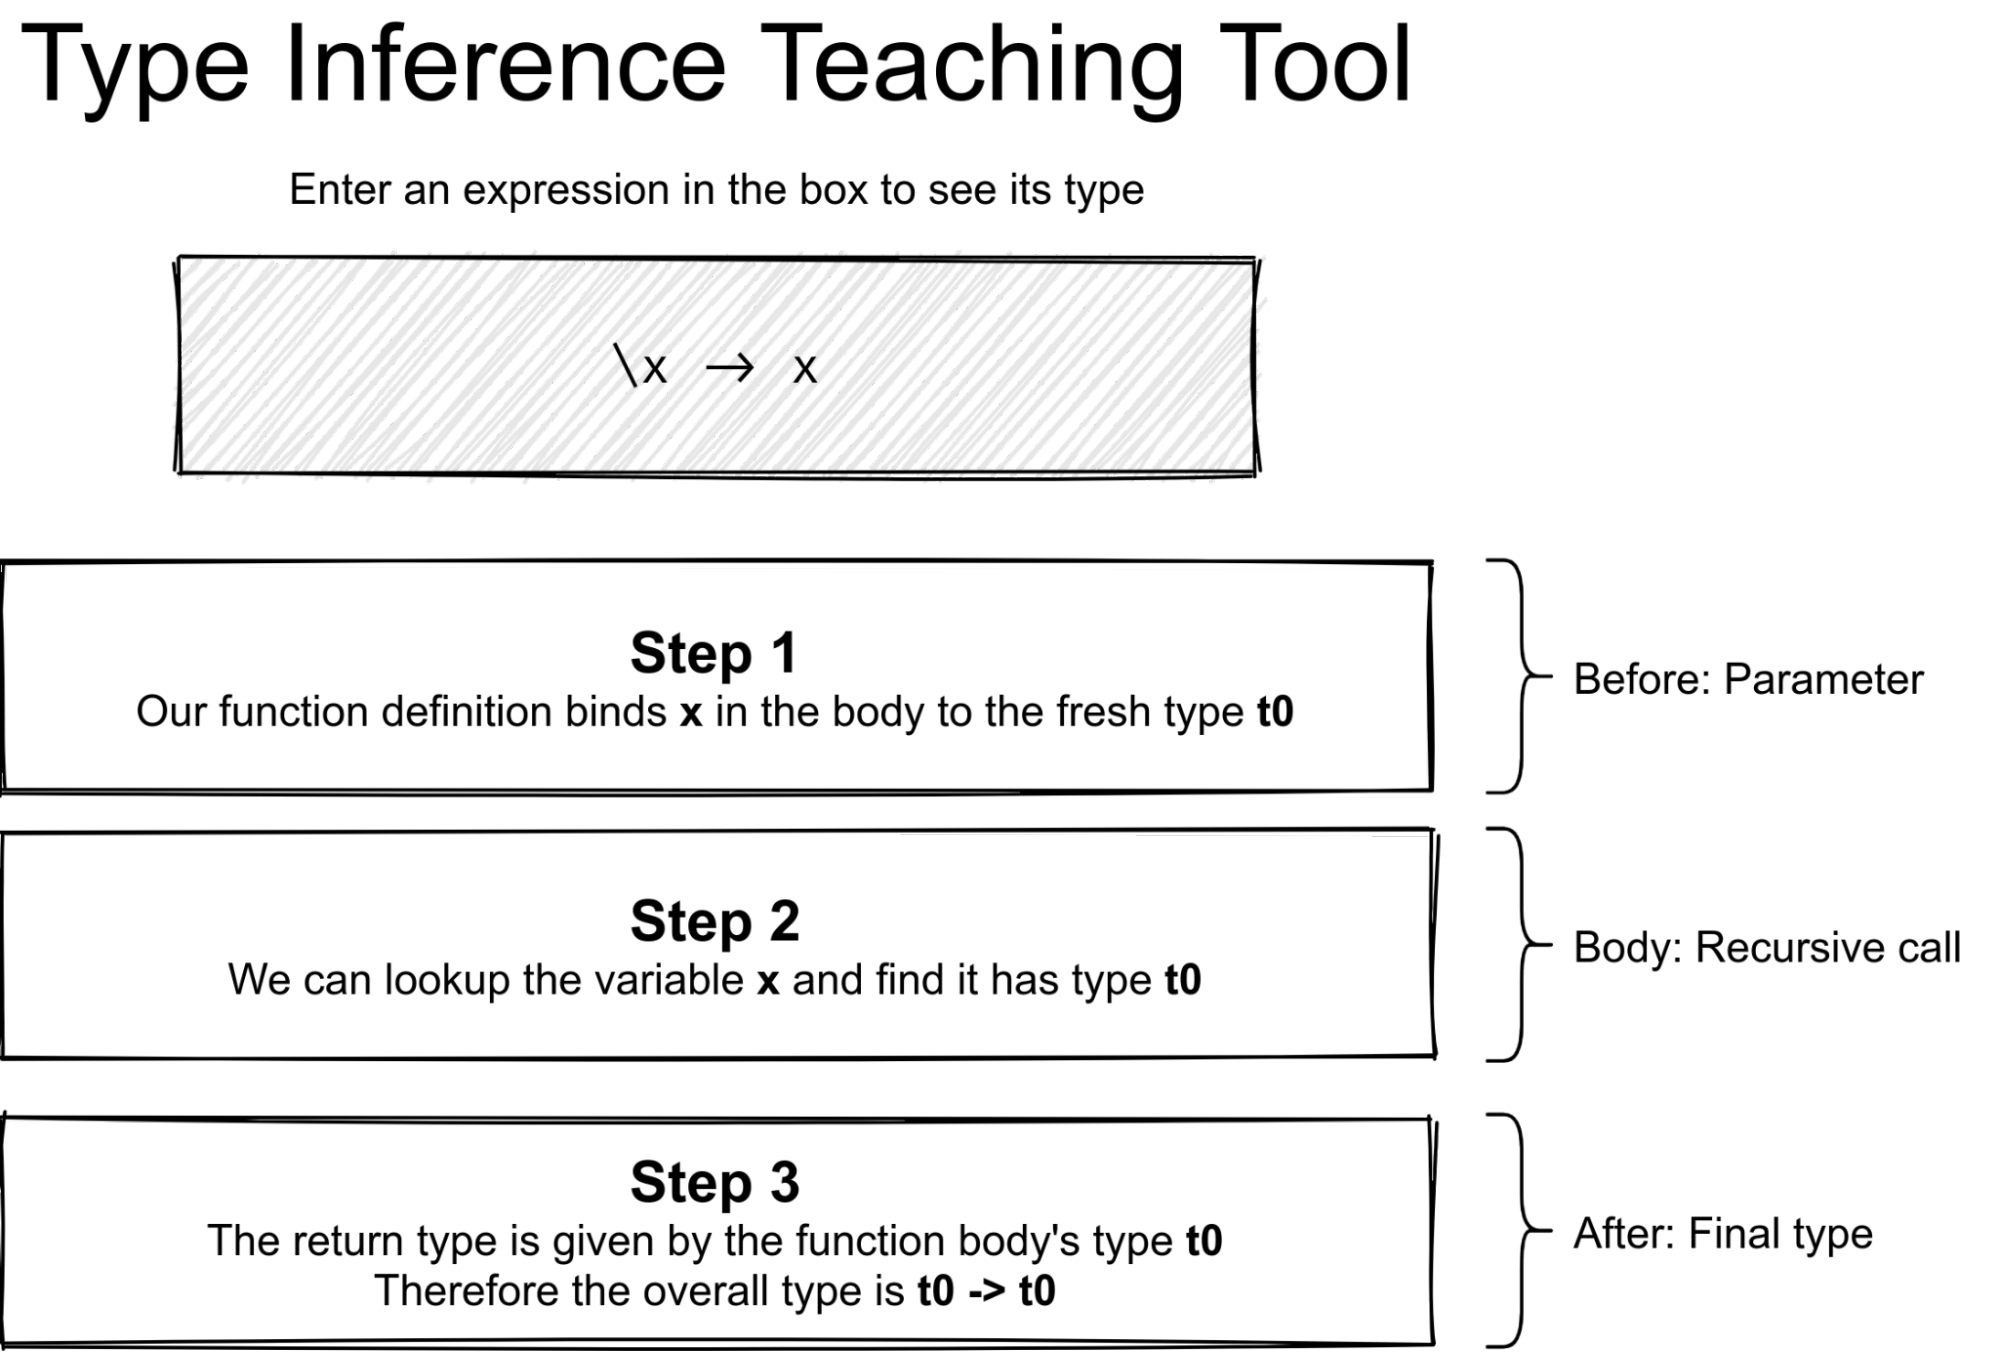
\includegraphics[width=\linewidth]{images/image8.png}
  \caption{The TypeScript playground, with an example from the type inferece documentation showing how class types work with the inference engine.}
\end{figure}

Programming language documentation and informal resources both are generally aimed at a more clearly targeted audience, usually programmers using a specific language. They are written in simpler language and use significantly less notation than formal resources which makes them easier reading. Their use of examples makes concepts clearer, and many of them have a level of interactivity which allows readers to try things for themselves, allowing readers to test their own knowledge or verify something that isn’t clear to them from the documentation alone. For example TypeScript's documentation allows users to hover over code samples to inspect the types as well as open it up in an online coding environment, while Golang and Rust's respective documentation sites have example programs which users are encouraged to edit and run online. Blog posts often have code snippets or GitHub gists for users to run, and in talks presenters may give live coding demos, which serve similar purposes.

\begin{figure}[h!]
  \centering
  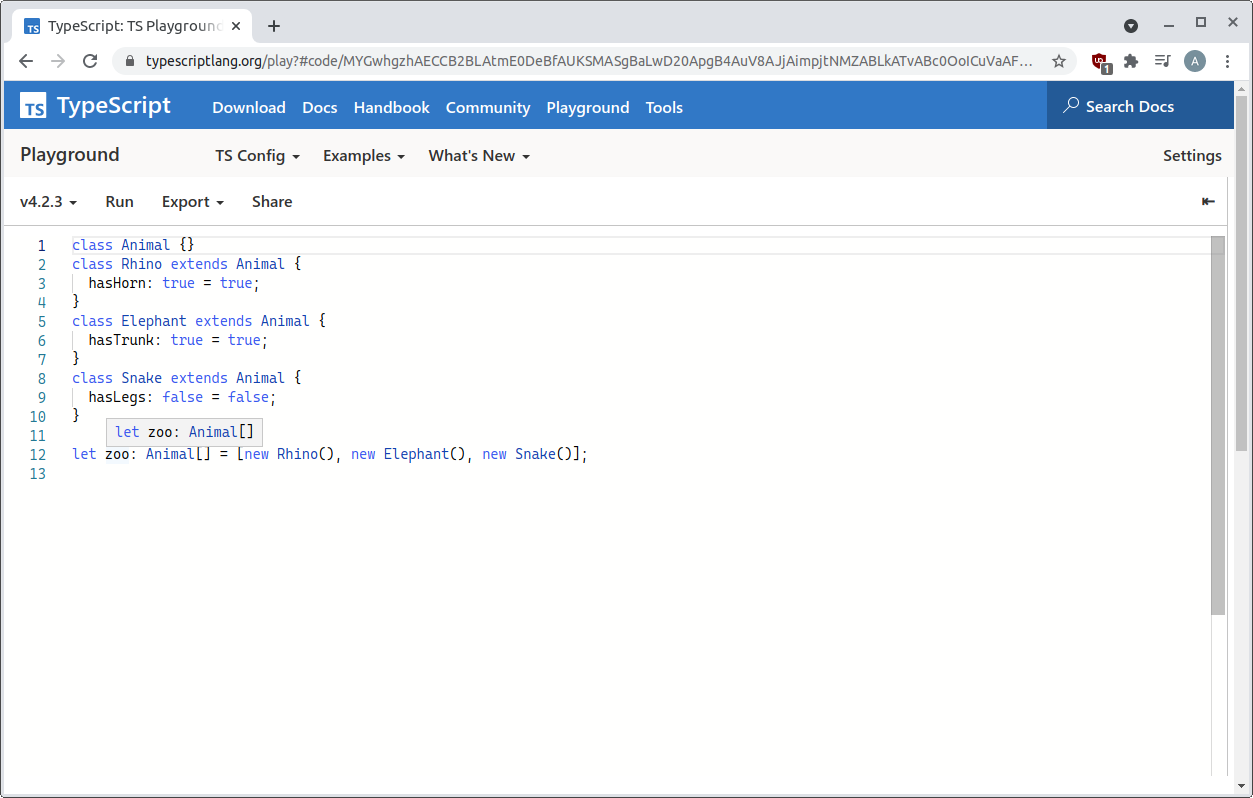
\includegraphics[width=1.000\linewidth]{images/image5.png}
  \caption{Golang's limited type inference is explained in 'A Tour of Go', with an example program the user is prompted to edit and run.}
\end{figure}

\begin{figure}[h!]
  \centering
  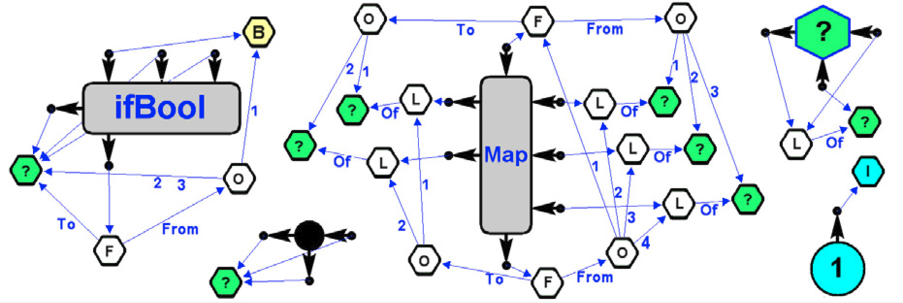
\includegraphics[width=1.000\linewidth]{images/image24.png}
  \caption{Rust's page on type inference is short, but has a well-commented and insightful example that can be run and edited inline in the browser.}
\end{figure}

Formal resources are usually aimed at a more mathematically-inclined audience, with less specific focus on any language or technology. They often use mathematical terms and notation to convey ideas, which some readers may find difficult to understand. In particular, papers are often written in a very precise and succinct way with few examples, which can make them hard to interpret. This is likely due to the length constraints put in place by academic journals which incentives authors to cut more detailed explanations and examples from their work. Few papers and lecture notes would be immediately accessible to the general computer scientist, as papers often assume the reader has a strong grounding in the field already and lecture nodes are meant to be read in order, expecting the reader to have read the previous 20 lectures worth of notes. However, they do usually give clear and useful references for background and further reading which is useful for in-depth research on the topic, if not for an introduction. The implementation of a type inference algorithm and how it is applied to a specific language is rarely discussed. Where it is discussed the only languages used were Haskell, ML and OCaml. According to the StackOverflow Developers Survey\footnote{\underline{\href{https://insights.stackoverflow.com/survey/2020\#technology-programming-scripting-and-markup-languages}{https://insights.stackoverflow.com/survey/2020}}} Haskell is used by 1.8\% of professional developers, while ML and OCaml are very rarely used in practice. These examples may therefore be of limited use to explain to developers how type inference is used in languages they are familiar with.

Finally, the different nature of resources means some are harder to correct or update with new information.

Informal resources generally seem to have the most errors, likely because they have little review process and may be written by anyone. Sometimes through comments other readers can provide corrections or clarifications, but these are not always incorporated into the material. Moreover, commenting is not always available and also given the specific nature of some content few people are likely to view and suggest corrections to the content. Additionally, as informal resources are usually published as one-off talks or blog posts, it is rare for the document to be maintained and kept updated which can lead to inaccuracies if the underlying technology they are discussing has made breaking changes to its implementation.

Programming language documentation on type inference is generally accurate and well maintained. It is kept up to date with changes to the language, as usually there is a requirement to keep documentation updated in programming language projects. Additionally, almost all programming languages are open source and welcome external contributions to their documentation so readers are able to suggest improvements or raise issues about inaccuracies. Generally there is a review process, often requiring a maintainer of the programming language to approve the changes before edits are made.

Formal resources generally have few errors. For academic papers, this is likely a result of the peer-review process. Lecture notes are generally written by academics with relevant qualifications and educational backgrounds, who are likely to be knowledgeable on the subject. However, academic papers and lecture notes are unlikely to be updated, which means any inaccuracies in them are harder to correct. Exploring the literature we found some papers on type inference with errors which make understanding them fully more difficult. Finally, online encyclopedias can be reviewed and edited by many people, whose combined expertise generally results in accurate articles although they are prone to errors being introduced by even just a single contributor if they lack a review process. Formal resources are less likely to become outdated with time compared to informal resources. This is because formal resources focus on the more general underlying concepts over discussion on a specific implementation.

This exploration into existing teaching resources is summarised in the table:

\begin{adjustbox}{center}\begin{tabularx}{1.2\textwidth}{ |p{2cm}|X|X|X| }
  \hline
   & \textbf{Content} & \textbf{Accessibility} & \textbf{Correctness} \\
  \hline
  \textbf{Language docs} & Explains how type inference is applied in the context of a specific programming language including error cases. & Written in plain language with many code samples and often interactive environments. & Few errors, and generally well-maintained. Content may change as rules of the language do. \\
  \hline
  \textbf{Formal\newline resources} & Explains how type inference works at a general level. & Uses complex notation and requires significant background reading, and is sometimes brief at the expense of clarity. & Few errors, although errors that do exist can be hard to correct. Usually relevant for a long time. \\
  \hline
  \textbf{Informal resources} & Contains practical tips, however usually very specific and irrelevant to many programmers. & Written in plain language with many code samples. & Inaccuracies are common, and often go undetected or unresolved. Can become outdated quickly. \\
  \hline
\end{tabularx}\end{adjustbox}\\

TODO: (maybe?) discuss my exploration of existing teaching tools (wolframalpha, khanacademy, cymath, microsoft math, css diner)

This research into existing resources identifies strengths and weaknesses of different approaches. Given that this project is a one-off piece of work and the end product may not be maintained indefinitely, research into the content, correctness and longevity of resources suggests that the focus should be on the more general type inference concepts rather than specific programming language features. The tool should support error cases, not just correctly-typed expressions. It should be reviewed by my project supervisor tested with users to identify errors that can be resolved before project completion. To aid accessibility text should be written in plain language, the tool should offer several insightful examples and the output should avoid overuse of complex notation.

As a tool that displays the output of type inference algorithms, to further determine the user interface for the output of the tool the presentation of type inference proofs is examined. My supervisor initially gave some examples of worked proofs for type inference, which also matched the format of proofs found in papers and in online resources. These proofs are broken down into steps, which each look at a particular subexpression and apply a certain typing rule. Depending on the type of proof (whether it is based purely on the typing rules or is more procedural and similar to an algorithm), this may also result in explicit unification resulting in a substitution to be applied.

Based on this, the tool is designed to show the result of type inference on an expression broken into steps. Given that the tool will be automated, the steps must be generated based on some deterministic procedure and so the steps will correspond to those of the type inference algorithms. This means the steps will need to show the unification operations performed and the resultant substitutions to fully explain how the types are being inferred.

A basic UI mockup is shown below that takes an input expression and displays the inference algorithm steps beneath it. While simple, it is fundamentally similar to the final design of the application. It was also at this design that it was decided to show the type derivation feedback instantly on the same page, based on the limitations of previous related work and the strength of interactive playgrounds in programming language documentation. On top of this design, the final application adds a choice of algorithms, several samples to choose from and a display of the final type. In addition, the final application shows and explains the steps of the type inference algorithm when type errors are present.

{\centering \begin{figure}[h!]
  \centering
  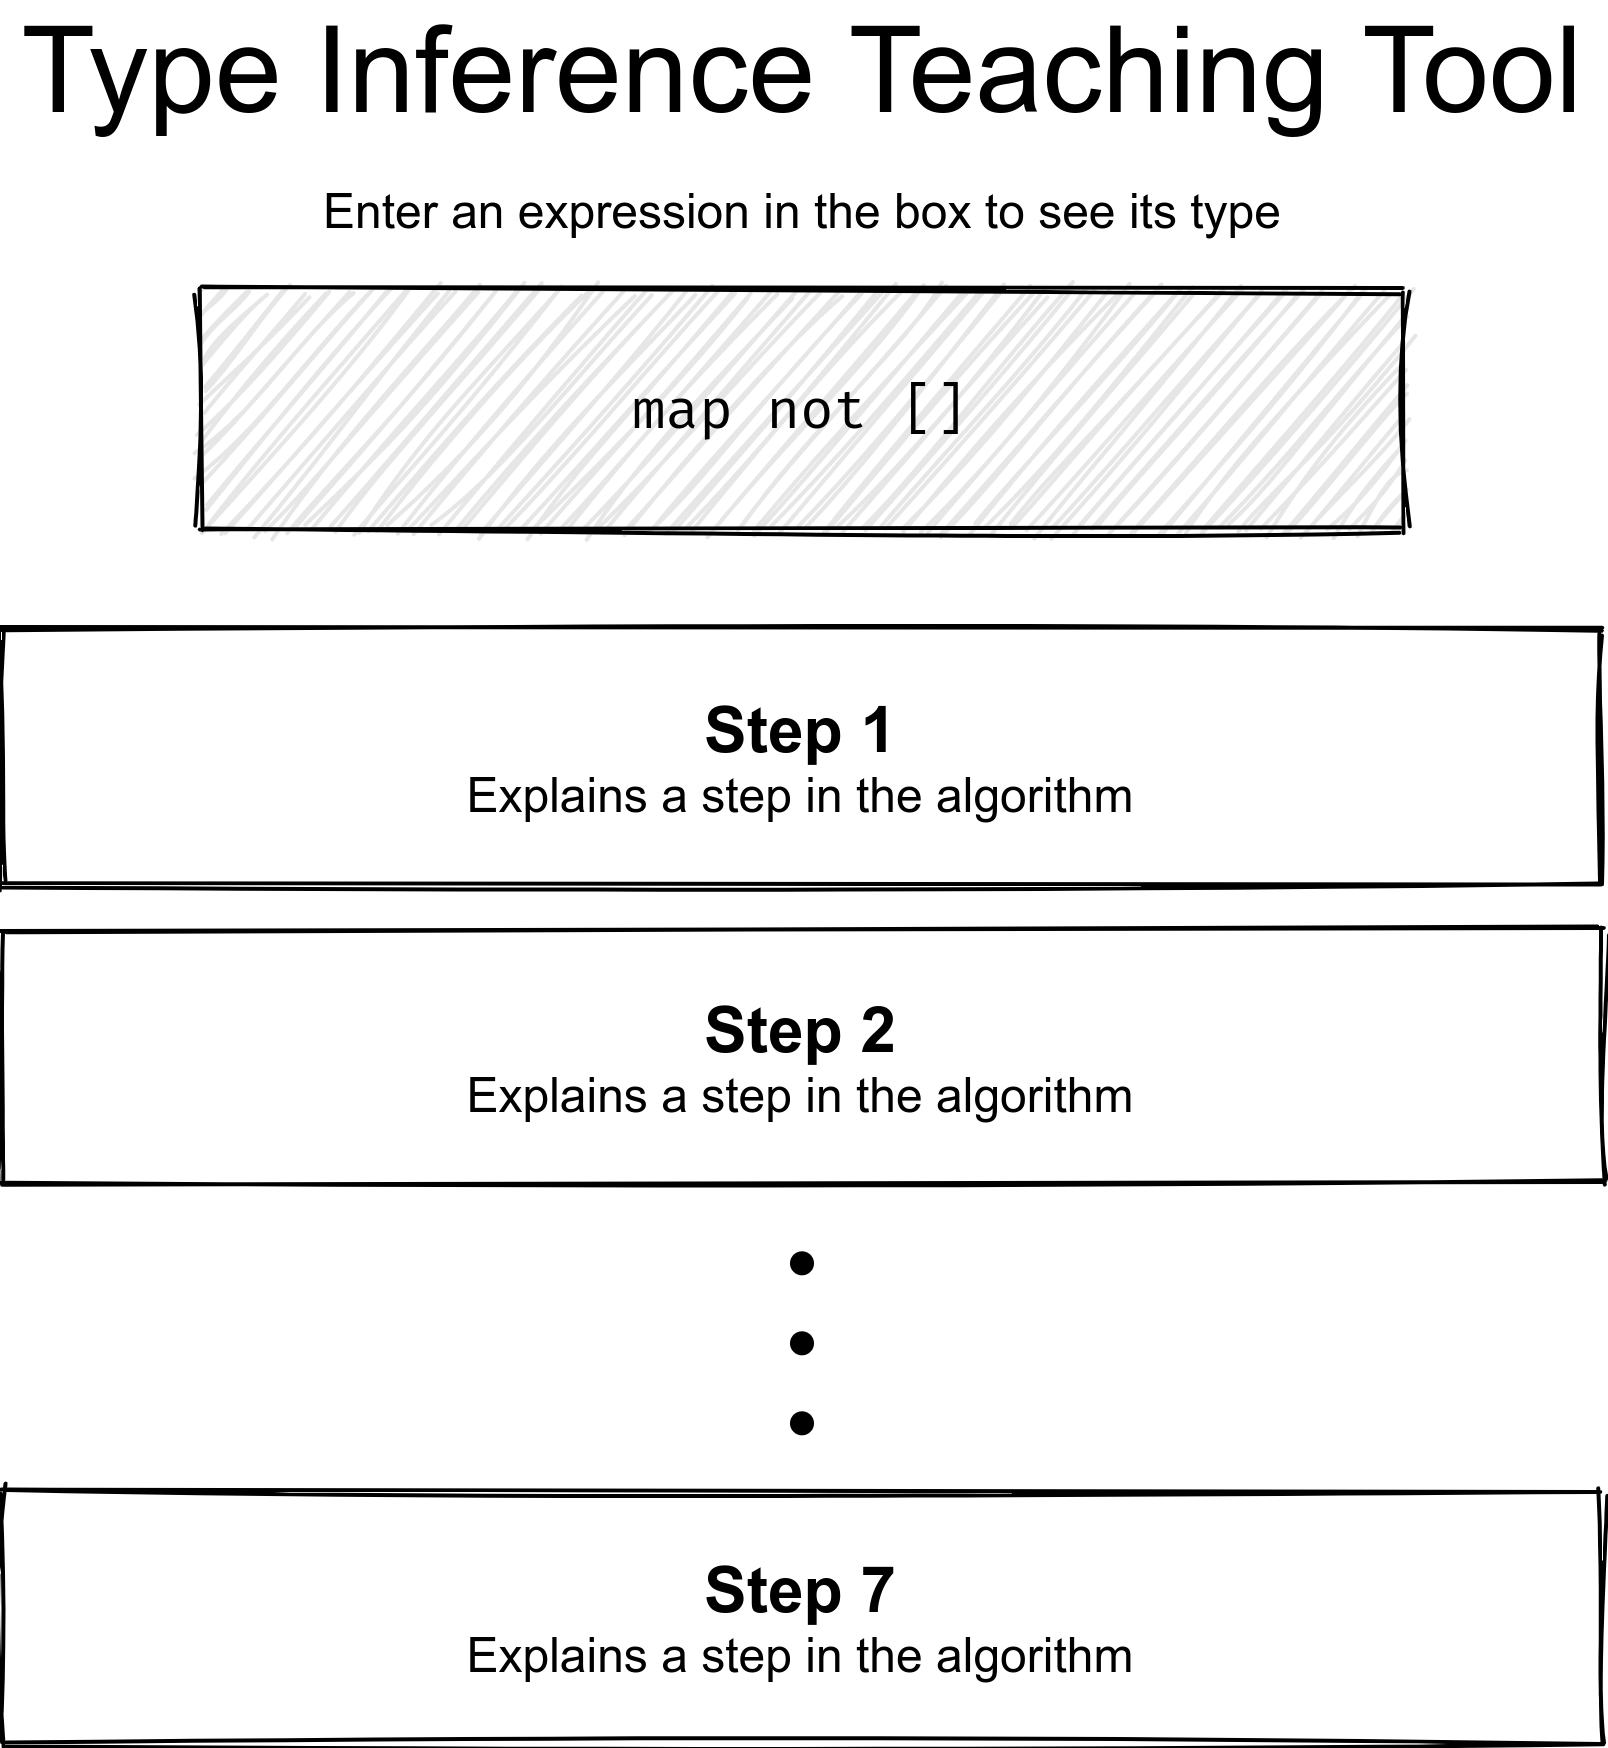
\includegraphics[width=0.756\linewidth]{images/image21.png}
  \caption{Recreation of an initial sketch of the UI for the teaching tool.}
\end{figure} \par}

A step in the UI generally corresponds to a rule of the type inference algorithm. As the type inference algorithms are recursive, some rules may call the type inference algorithms again on a subexpression. In these cases it may be necessary to split rules of the type inference algorithm up into two parts, before and after a recursive call. This helps ensure the ordering of the steps makes logical sense.

For example, this happens with function abstraction in algorithm W: the before step shows assigning a new type variable as the parameter’s type, steps between show the results of the recursive call to the body, while the after step details the final type of the function abstraction expression.

{\centering \begin{figure}[h!]
  \centering
  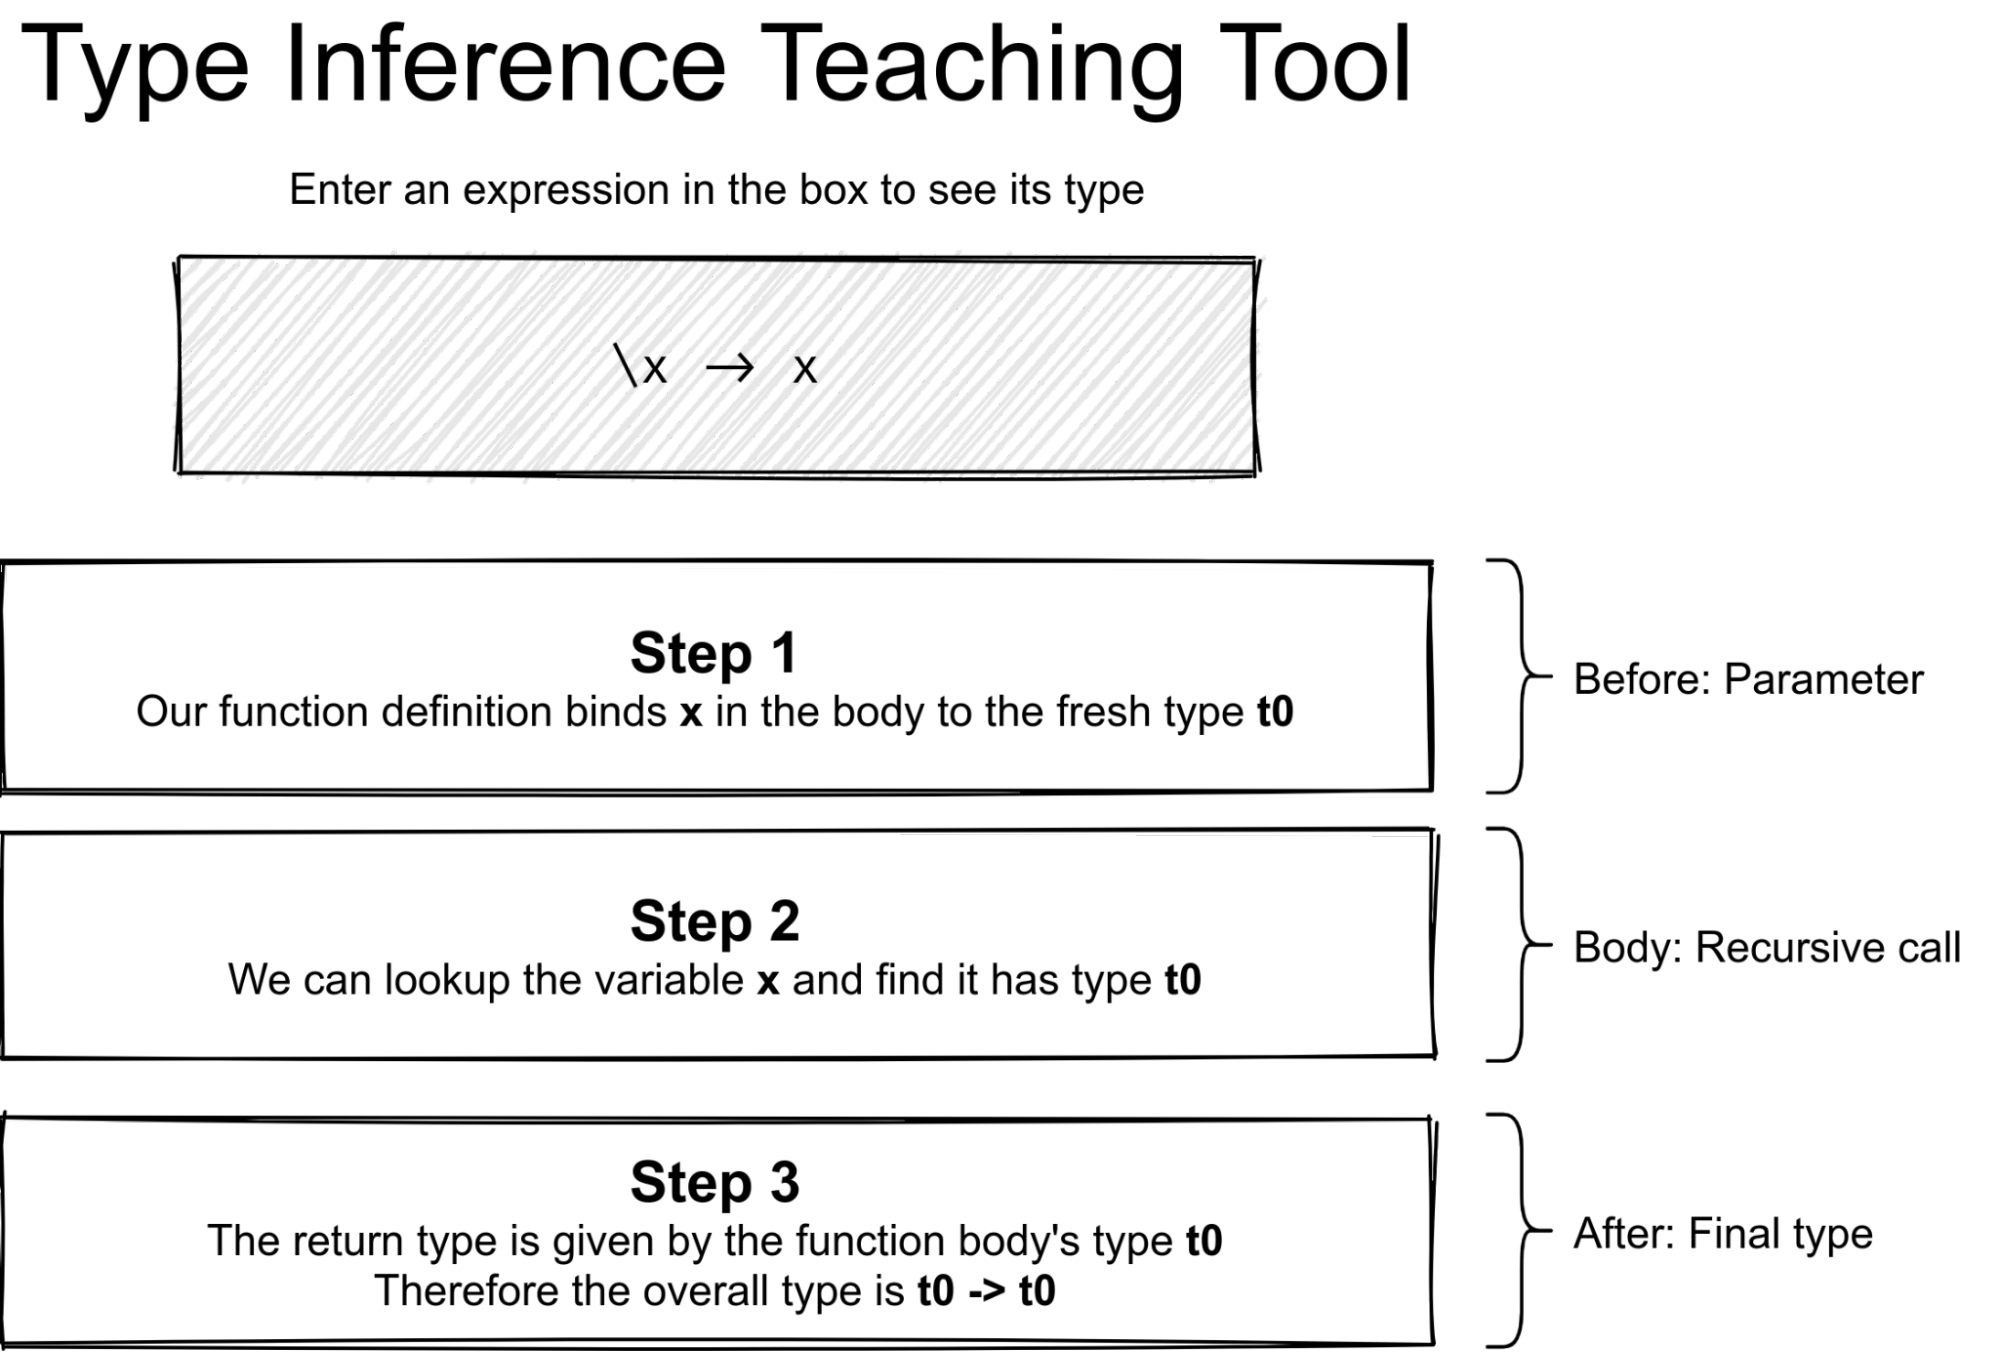
\includegraphics[width=0.945\linewidth]{images/image15.png}
  \caption{Function abstraction in algorithm W requires two UI steps to represent one rule of the algorithm}
\end{figure} \par}

In addition to the rule steps, algorithm M requires an extra beginning and end step. These are required as algorithm M requires an input type and does not return a type respectively. The first step is to create an initial new type $t_0$ for the root node, and the final step is added to apply the final substitution to type $t_0$ (effectively the value of $t_0$ from the substitution).

{\centering \begin{figure}[h!]
  \centering
  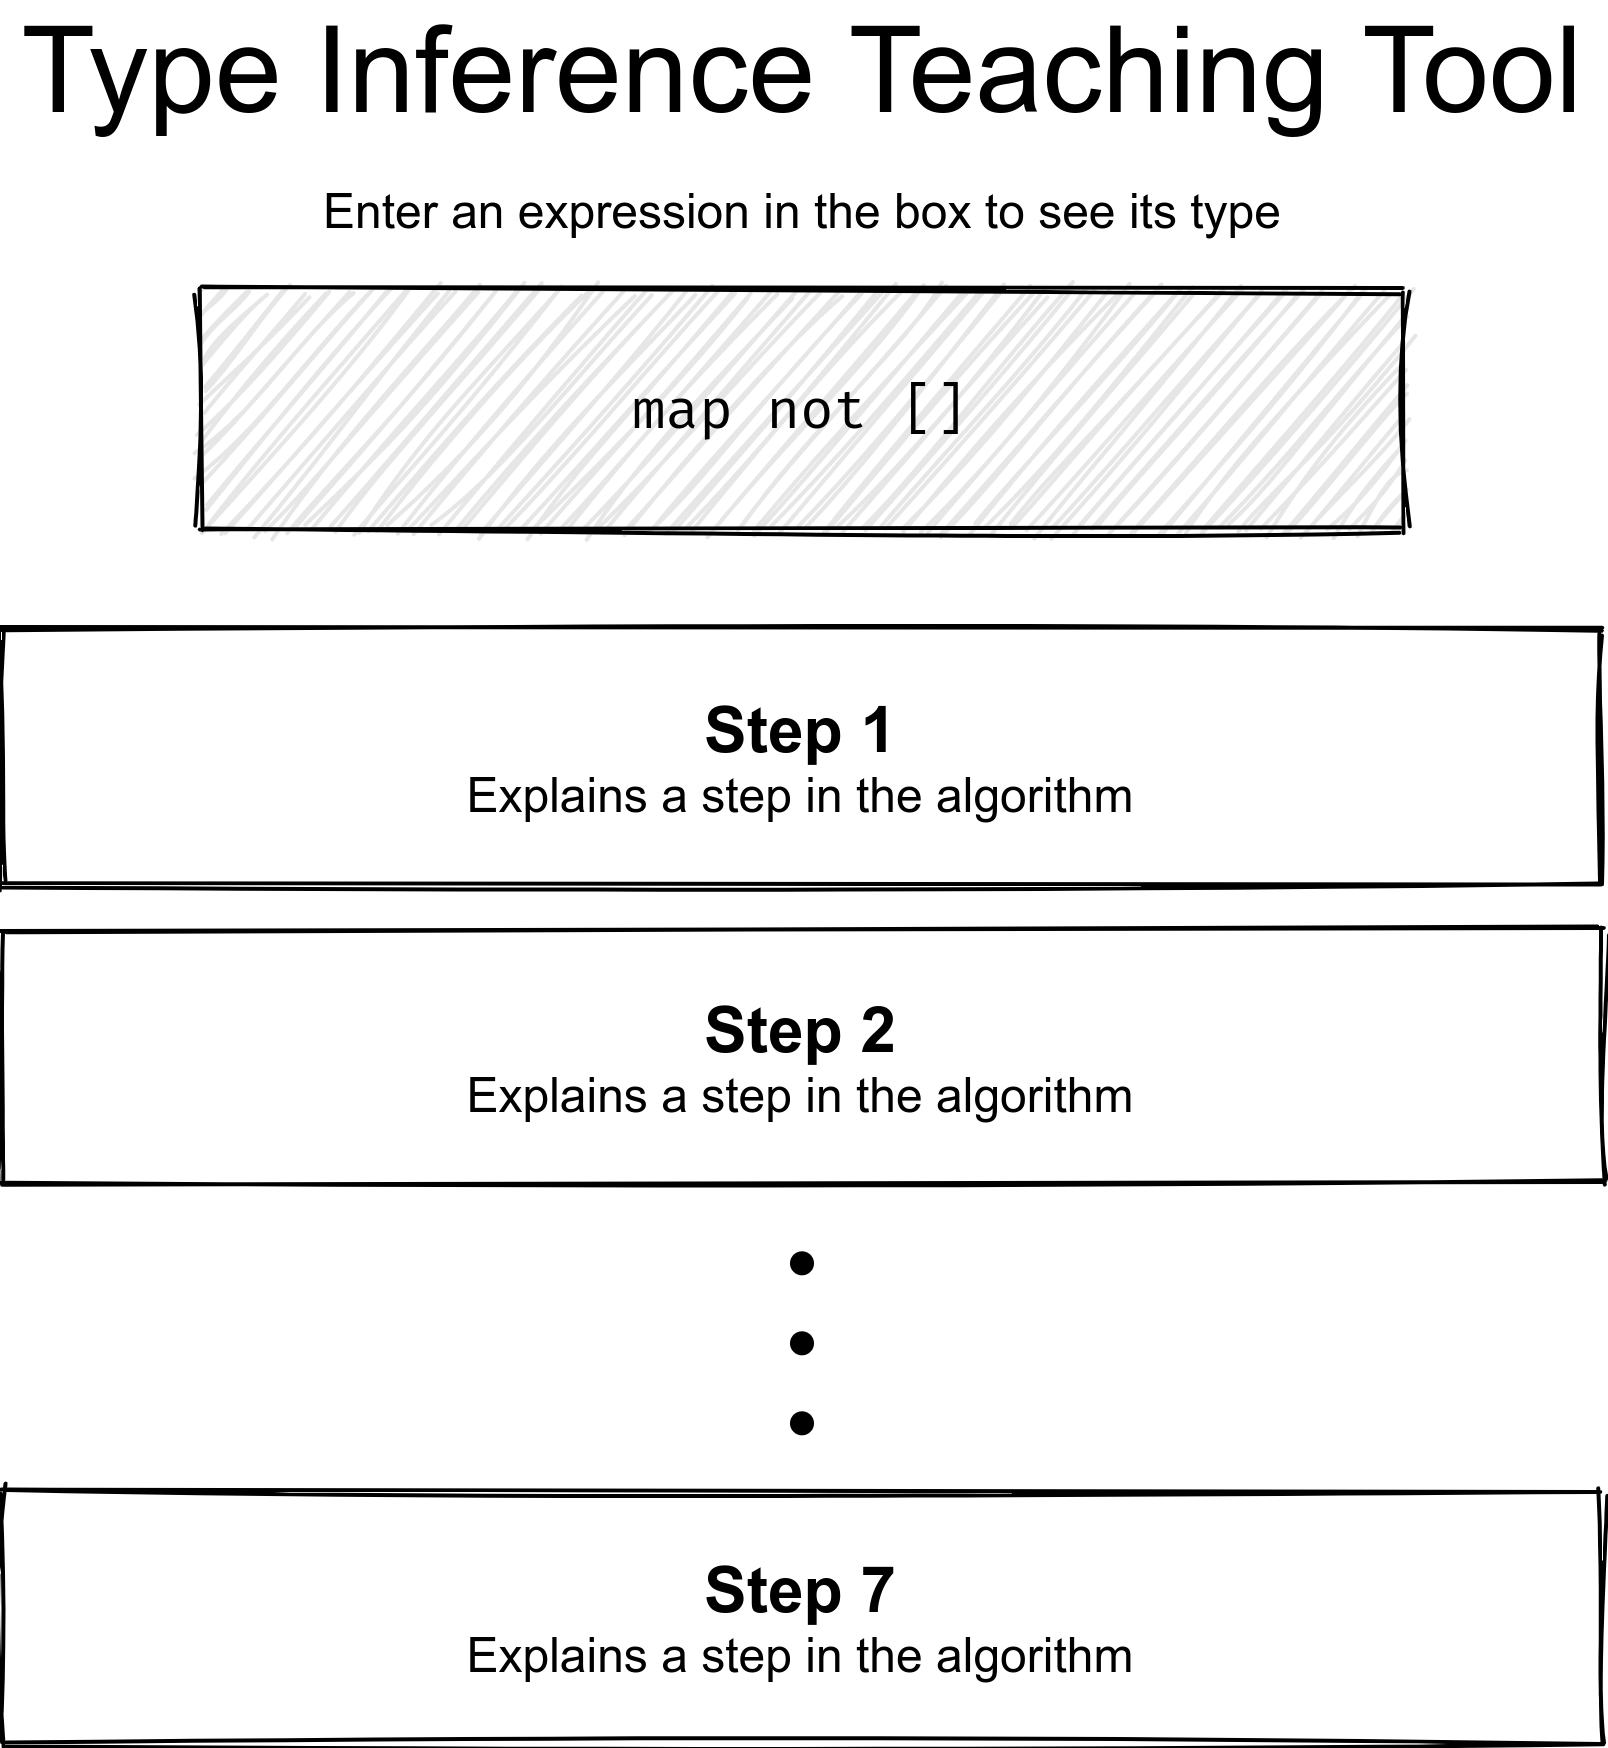
\includegraphics[width=0.960\linewidth]{images/image10.png}
  \caption{Algorithm M requires an initial and final step.}
\end{figure} \par}

To make it clear what part of the expression each step relates to, a representation of the expression as an AST with the relevant parts highlighted is shown at each step. The visualisation is computer generated and must fit in a fixed width space, and as such a vertical design was chosen to represent it. In this design, each box represents a tree node and the boxes are ordered in a vertical list. Nodes may have children, which they are attached to with edges to the left of the children.

{\centering \begin{figure}[h!]
  \centering
  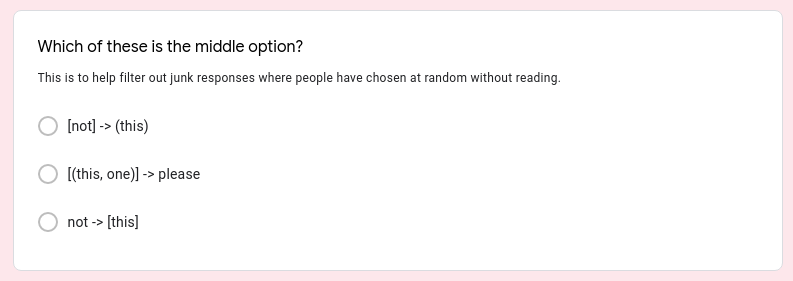
\includegraphics[width=0.357\linewidth]{images/image31.png}
  \caption{The expression \mintinline{text}{let x = 3 in odd x} may be represented by this vertical AST.}
\end{figure} \par}

This vertical design was chosen over a horizontal design due to the space constraints of the tool page, and the difficulty in implementing a consistent and well functioning horizontal tree visualisation algorithm.

{\centering \begin{figure}[h!]
  \centering
  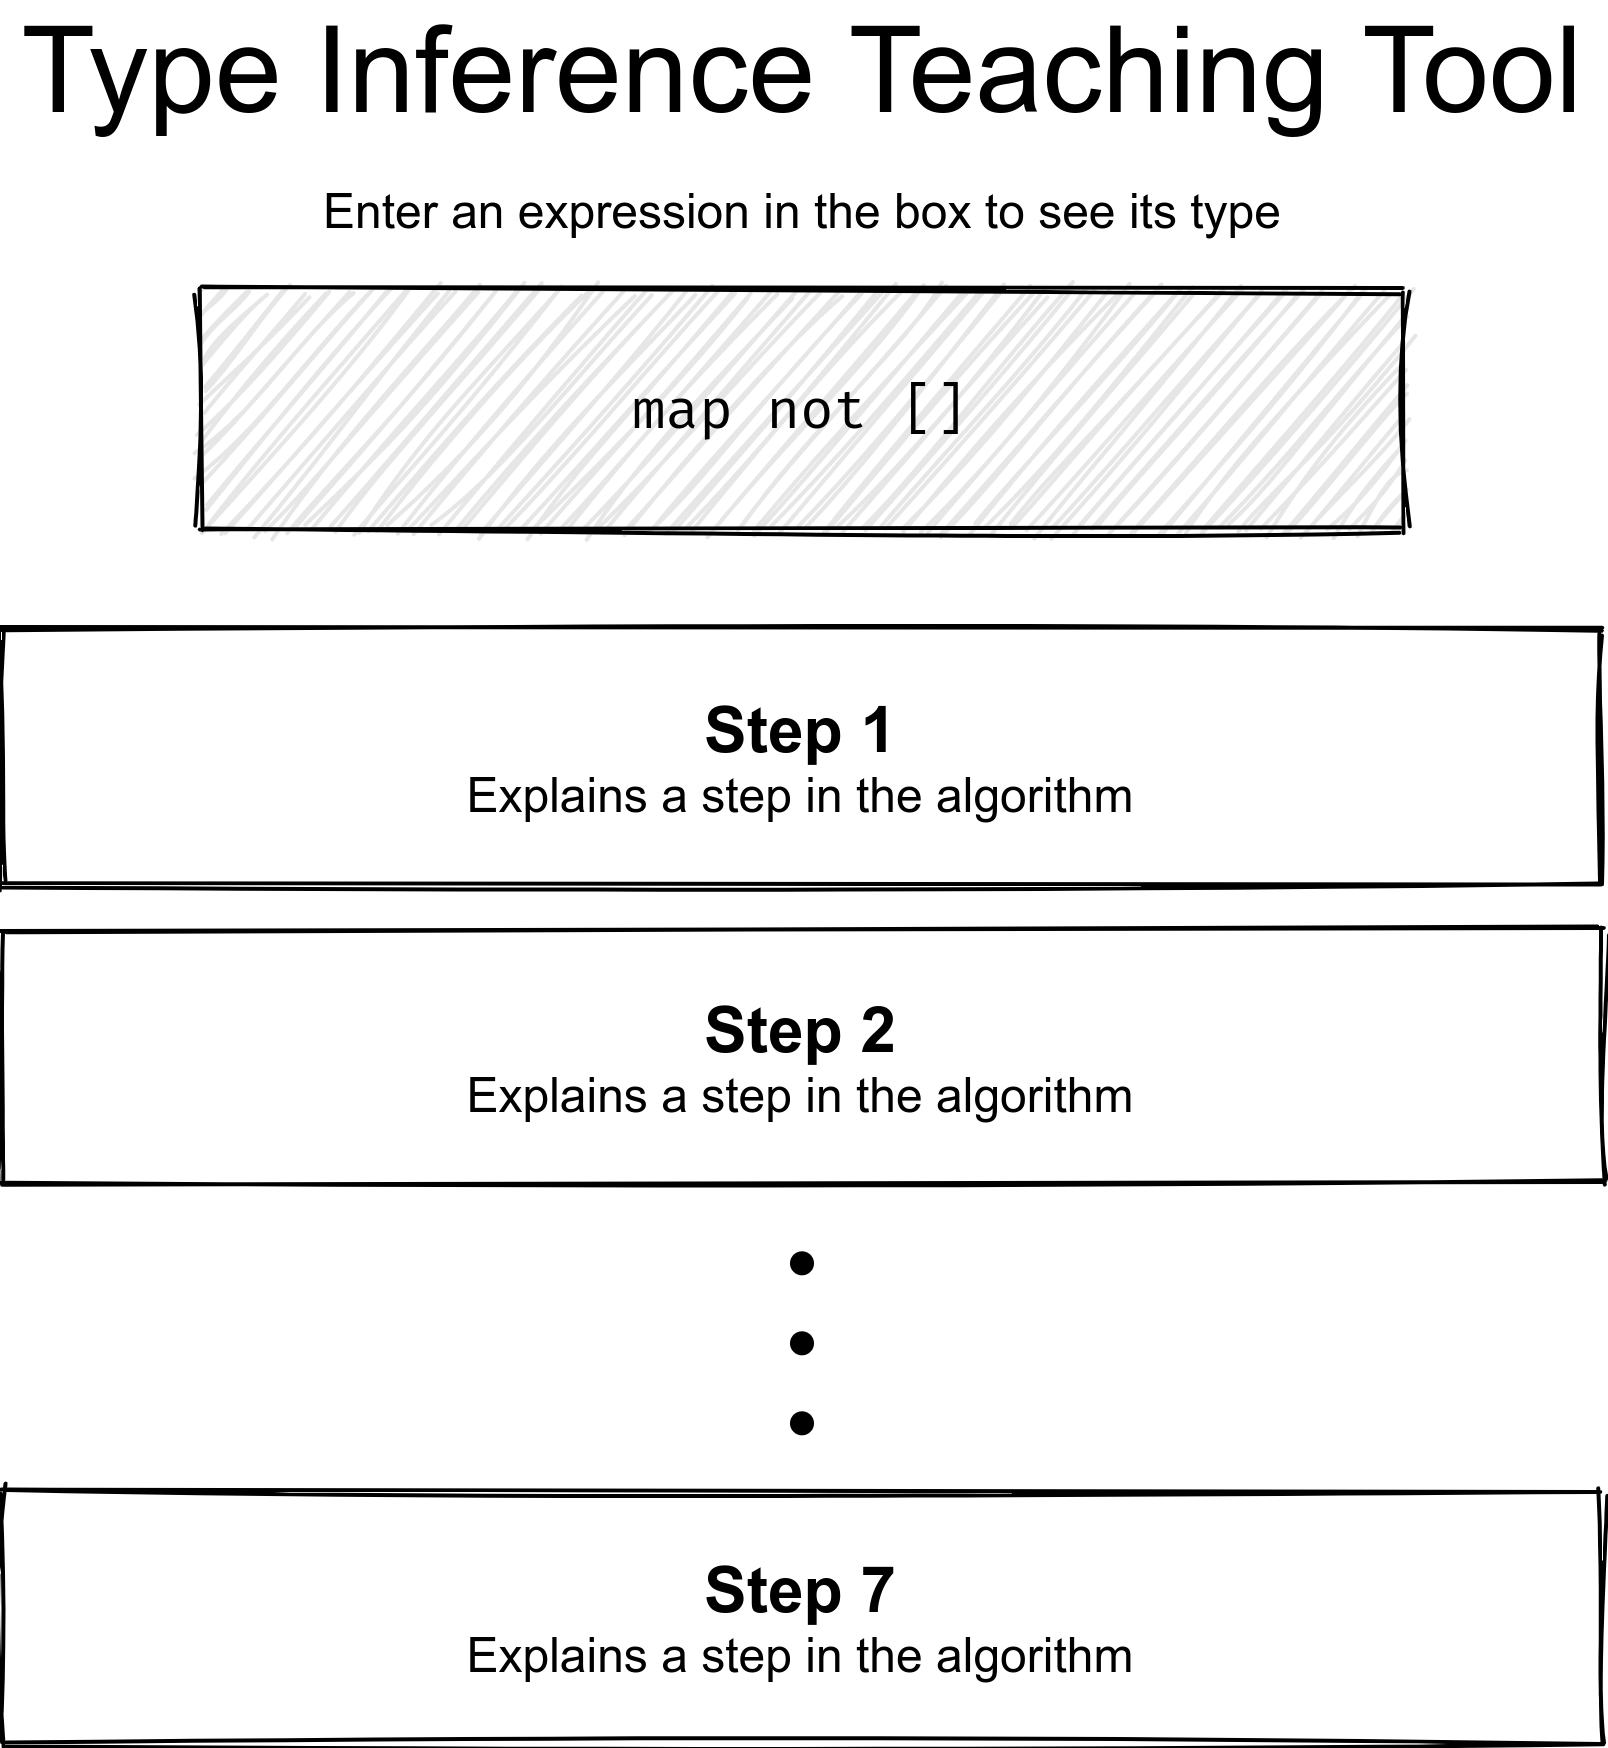
\includegraphics[width=0.813\linewidth]{images/image13.png}
  \caption{Example of what a more horizontal design of AST might look like.}
\end{figure} \par}

Showing ASTs is preferable to just showing the relevant subexpression as it makes it clearer what part of the whole tree is being analysed. Showing ASTs is also preferable to showing the full expression and highlighting only the relevant part as it better demonstrates how the program is broken into its constituent parts, is clearer for showing syntactically-sugared features such as lists, and relates it to the original type inference algorithms more closely as users can see how similar AST structures follow similar type inference rules.

{\centering \begin{figure}[h!]
  \centering
  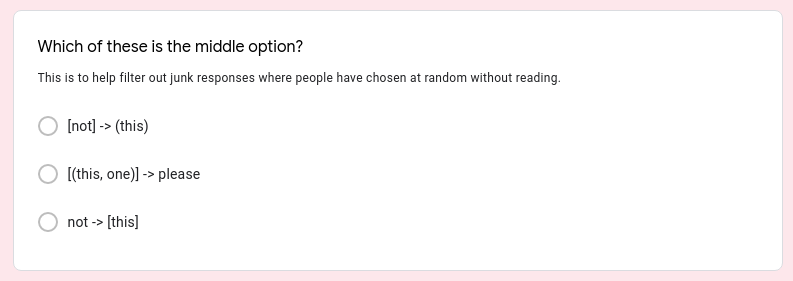
\includegraphics[width=0.884\linewidth]{images/image26.png}
  \caption{Hovering over the 'function application' node highlights the corresponding subexpression in the entered program.}
\end{figure} \par}

To help relate the ASTs to the entered expression, when a user hovers over a part of the AST the matching part of the entered expression that corresponds to the hovered AST node is highlighted. For consistency and to help users understand larger subexpressions too this also works for non-leaf nodes of the tree.

A web interface was chosen over a desktop program to maximise compatibility across devices, so the resource was accessible to as many students as possible. This allows the resource to work on platforms including Windows, Mac, Linux, iOS and Android. In addition, a web interface makes the tool easier to share and setup, as users simply need to navigate to the site rather than install a native application. It is also easier to copy and is more likely to be compatible with future platforms, increasing the tool's longevity, a characteristic highlighted as important earlier in this section.

While access to certain APIs is more limited in a web application compared to native applications, this did not limit any of the application's proposed features so was not a concern.

A native application would be likely to have better performance (in terms of computation time), however it was believed that the web application would not encounter serious performance problems on reasonable inputs. In later performance testing few concerns were raised about the applications performance, and those that were could be mitigated (as detailed in the implementation chapter). Feedback from user testing supports this, with one respondent commenting that the application felt ``very fast''.

\section{Architecture}\label{id:h.l33hnjbawceh}

The software is designed as interchangeable, loosely-coupled modules to make it easy to adapt and extend. This gives the project freedom to change over time in response to feedback, without having to redevelop common functionality.

TODO: insert module diagram

The alternative module structure considered was to have the type inference modules standalone, to avoid depending on the language core. They would then be parameterized with methods to extract the necessary data from any AST model, promoting flexibility. However, this would introduce significant complexity and performance overhead for little gain as the language core is fairly lightweight. In addition, it would have meant utility functions, types and models could not be shared in the language core between type inference modules, meaning they would need to either have another separate module for shared utilities or have a large amount of code duplication.

TODO: insert alternate module diagrams

The downside to splitting the project up into several modules is the tooling is a little more complex. Modules must be built separately and in the correct order which is slightly slower than compiling one larger app, and IDEs have to be set up to understand how to navigate between the modules. However, this is outweighed by the maintainability and extensibility benefits of keeping functionality in separate modules.

\subsection{Choice of programming language}\label{id:h.dj2rwwqr30vu}

The modules are all written in the same language, so that they are compatible and easy to get working together. Additionally, using one typed language allows for type-checking across modules to ensure API calls are valid and their results are used correctly. To write a modern web application, a JavaScript-compatible language is the obvious choice as it is supported and promoted by all major browsers. TypeScript was chosen for this for several reasons.

TypeScript is a statically-typed language which transcompiles to JavaScript that can be run in the browser. As a typed language, it provides the benefits of types listed earlier, which is important when dealing with a codebase with several modules. TypeScript was therefore chosen over plain JavaScript, which lacks compile-time typechecking.

Elm, CoffeeScript, PureScript and Dart are other languages that compile to JavaScript, however they lack as rich package systems which can provide useful utilities and dependencies. Furthermore, Dart and Elm are largely focused on the presentation of data, so while it would be possible to write reusable independent libraries for type inference in them, it would not be easy.

Of the browser-compatible languages, TypeScript is the second most used after JavaScript itself (according to the StackOverflow developers survey\footnote{\underline{\href{https://insights.stackoverflow.com/survey/2020\#technology-programming-scripting-and-markup-languages}{https://insights.stackoverflow.com/survey/2020}}}) and so developing and publishing packages in TypeScript may be useful for a wider audience.

Lastly, my previous experiences with both TypeScript and the other languages informed the decision. Familiarity with TypeScript played a key role in using it over other languages targeting the browser.

\subsection{Language core}\label{id:h.hggmfighusoc}

The base module, which all other modules depend on is the language core.

The language core contains key models, which are used throughout the rest of the software. These models represent AST nodes, types, contexts, substitutions and other results from type inference algorithms. It also defines the interfaces for modules containing type inference algorithms.

In addition to these models, it contains a default context with types for many common functions. This context is based on Haskell's Prelude, which makes it easy for learners familiar with Haskell or similar functional programming languages to use the tool.

The language core also holds key helper functions such as utilities to create types. For example, callers can construct an instance of a type with:

\begin{minted}[breaklines]{typescript}
tuple(char, boolean)
\end{minted}
instead of

\begin{minted}[breaklines]{typescript}
new TypeFuncApp(',', new TypeFuncApp('Char'), new TypeFuncApp('Bool'))
\end{minted}
There are also helper functions to combine and apply substitutions, as well as to perform unification. These helper functions can be tested independently, verifying the correctness before using them in dependent modules. Testing is discussed in more detail in the implementation chapter.

Lastly, the language core contains a lexer and parser. Together, these take an input program as a string and return an AST, or report that the program is syntactically invalid. The lexer splits the input string into tokens, while the parser operates on this stream of tokens to recognise higher-level program constructs and construct the AST nodes.

A parser combinator library is used to perform the lexing and parsing. A parser combinator library was chosen over a recursive descent parser or an LL, LR or LALR parser generator as it was recommended by my supervisor and several online sources discussing implementing functional language parsers. In addition the software needs to be compatible with running in the browser which most LL, LR and LALR generators do not support. In addition, none of these types of generators provides output that is easy to implement for the browser or debug manually, whereas parser combinators are relatively easier to implement by hand.

The library chosen for lexing and parsing is Masala, one of the few parser combinator libraries implemented in JavaScript. Masala is based on Haskell’s Parsec library, is tested for the browser and is well-maintained. In addition, it has strong TypeScript definitions which support its integration into the typed language module. Other libraries including Parjs, Parsimmon and Chevrotrain have weaker documentation, and Parsimmon lacks complete TypeScript type definitions. Some other libraries like Jison and Nearley cannot easily output the custom AST node classes, while Masala can. This feature also helps extract the location of nodes in the source program to support being able to highlight where in the input expression an AST node has come from.

\subsection{Type inference algorithms}\label{id:h.75leuokwbltp}

On top of this language core are type inference algorithms \W, \W' and \M. Given an AST representing an expression, they return either a type or an error explaining why they were not able to infer the type. Along with these, they can also optionally return a sequence of steps taken as part of the algorithm. Each step includes a message and AST to be displayed, with appropriate parts of the AST highlighted.

Each type inference algorithm shares the same interface, allowing them to be used interchangeably. This means new algorithms conforming to this interface can be added to tools using the type inference algorithms, such as the web application, by simply changing the type inference library installed. Sharing the same interface also means that high-level module tests that call only the common function signature and assert on the final type can be shared across all the inference algorithms as they should all return the same type result, even if they take different steps to get there. This makes the development of tests easier so more can be written, and asserting the final types are the same across a number of varied cases improves confidence that the algorithms are implemented correctly.

Publishing the type inference algorithms separately helps keep the code clean and maintainable, and allows developers to only install the algorithms they need. While this does result in some code duplication, particularly between algorithm \W\ and \W', the benefits from keeping the modules small and easier to maintain individually make this trade-off worthwhile. Most of the common helper functions are already in the language core, which means the code duplication in the type inference modules is not excessive.

\subsection{Web interface}\label{id:h.q67ivlz7h61r}

Finally, depending on both the language core and the type inference algorithms is the web interface itself. This is the end-product that users interact with, implementing the user interface. Here users can type in a program, and view the steps the type inference algorithm took to infer its type. To do this, the web application passes the program to the language core which lexes and parses it into an AST, then passes that AST to a type inference library. The results of this are then shown to the user.

TODO: diagram of pipeline: user enters program as string, lexer lexes as tokens, parser parses to AST, type inference algorithm returns steps, web application displays them

The web application uses the React framework. Using a framework improves the structure of the code, as the application can be broken down into separate, independent components. These components can be reused to minimise code duplication, and can be individually unit tested with many testing libraries developed specifically for different frameworks. As well as this, using a framework in combination with a module bundler such as webpack makes importing and depending on other modules (such as the language core and type inference algorithms) simple. And in combination with a transcompiler that converts modern JavaScript to be backwards compatible, such as Babel, the application can be made to work for users with older browsers.

React was chosen over the alternative web frameworks Vue, Angular and Svelte. Vue and Angular are other popular frameworks, however for a single page application they are overly complex. In particular, Angular's component and dependency injection system, while useful in very large projects, would add significant unnecessary overhead to developing the system. The Svelte framework is different to React, Vue and Angular in that it avoids complex internal models, but instead compiles directly to simple JavaScript. This gives it better performance, but makes it harder to integrate with existing libraries and tooling. In addition, while Svelte supports TypeScript, this support was only added recently (July 2020) and is much weaker than React’s TypeScript support. Vue, Angular and Svelte are all significantly less popular than React (which is the most popular JavaScript framework). This means they have fewer available compatible packages and less community-developed documentation such as tutorials, guides or forums. In particular, Svelte is a new and much less widely-used framework, with less than 2,000 questions on StackOverflow compared to React’s nearly 300,000.

Create React App sets up the initial structure of the web application. Its starter template includes the required dependencies to build a React application, a variant of which also has TypeScript support. Using Create React App rather than starting from scratch allows the project to focus on developing the novel type inference teaching tool, rather than being too concerned with the setup of the tooling. However, using Create React App does limit how the build can be configured without choosing to ``eject'' (an irreversible process that makes the implicit build tooling explicit, but results in more maintenance). For example, while it installs Webpack and Babel to bundle resources and transcompile to JavaScript compatible with older browsers respectively, their corresponding configurations cannot be edited without an ``eject''.

The web application imports the type inference algorithms and the language core, and bundles them as part of the client application to be run entirely in the user’s web browser. A static site doing the processing fully client-side was chosen over a client-server architecture to reduce latency, minimise running costs and maximise the resource’s longevity. It also simplifies communication between modules, which otherwise would either need a manually specified or complex networking layer, such as using the proxy pattern with dependency injection. In addition, potentially complex models representing the AST would need to be reliably serialized and deserialized which is non-trivial when as classes they have member functions.

Performing calculations client side reduces latency as users do not need to wait on the network to transport data back and forth. Parsing and inferring the type of expressions in the browser takes tens of milliseconds, compared to hundreds of milliseconds that would be expected from a RESTful API. However, for particularly complex expressions where users have weak hardware (such as older smartphones), doing calculations client-side may be slightly slower than a client-server architecture. These cases will be rare, but happen when the networking-related overheads are outweighed by the difference in processing speeds between the server and client devices.

TODO: insert bar graph comparing average laptop, average phone, average server-client, older smartphone, high latency server-client

Avoiding dynamic calculations on the server means free static hosting sites such as GitHub pages can be used to serve the website. This significantly reduces running costs when compared to running a custom server to respond to requests, increasing the tools longevity.

The teaching tool’s longevity is further increased by serving a static artifact, as opposed to having dynamic server and client parts as a static website can easily be copied and archived. TypeTool, a related work that also aimed to explain type inference, was client-server based. However, the server has since been taken down and so is no longer accessible. As the lexing, parsing and type inference process was done server-side, archive websites like the Internet Archive’s Wayback Machine are unable to keep a copy of it, as they only store the static website content.

\section{Analytics}\label{id:h.60njhv340fb0}

To help evaluate the teaching tool and understand user behaviour, a system to collect and store behavioural analytics data is required. This tool should respect user privacy settings, minimize personal data collected (ideally data collected should be anonymous) and be able to view a single event stream to understand how a user is using the application.

Several popular existing analytics solutions were explored, including Google Analytics, Matomo, W3Counter, Simple Analytics, Angelfish, AWStats and Open Web Analytics.

The ``Do not track'' (DNT) browser setting is the simplest and most widely-supported way to indicate a user does not want to be tracked. However, Google Analytics, Angelfish, W3Counter, Open Web Analytics and AWStats do not respect DNT browser settings by default, and while possible in some cases to set up so that they do, this is difficult.

IP addresses are classified as personal data under the General Data Protection Regulations (GDPR). Some analytics tools such as Angelfish, AWStats, Open Web Analytics and W3Counter collect and analyse IP addresses as well as other personal data. This presents a problem for using these analytics tools within the EU, as users must be informed as to how their personal data is collected and processed, and users have several rights relating to personal data such as the right to be forgotten, the right to object or the right to access. In addition, many of these tools use cookies and similar on-device storage technologies to track users, which require consent under the UK’s Privacy and Electronic Communications Regulations (PECR). This would add significant unwanted overhead to the website for what is actually necessary.

To understand user behaviour, a single event stream that shows the different steps they took would be most useful. For example, seeing in what order they try out type inference examples and whether they view the more in depth documentation is much more useful data for evaluating and improving the tool than aggregate data about user demographics. Many platforms such as AWStats focus on the latter, and do not offer event stream (also known as `clickstream' or `clickpath') analytics. Some platforms like Google Analytics meet in the middle, offering event tracking but cannot present these in individual user streams. Angelfish offers event stream analytics, but does not support custom events, such as choosing a type inference example.

Finally the most practical concern is their running cost. Google Analytics and W3Counter are the only options with free plans, while other managed services such as Matomo Cloud and Simple Analytics are generally fairly expensive (both more than £275 per year for their cheapest plan). The cheapest available Angelfish license costs over £1,000 a year, and along with `free' options AWStats and Open Web Analytics needs to be hosted on a server which would incur server running and maintenance costs.

These factors can be summarised in a comparison table:

\begin{adjustbox}{center}\begin{tabular}{ |l|l|l|l|l| }
  \hline
  \textbf{Service} & \textbf{Obeys DNT} & \textbf{Anonymous} & \textbf{Event streams} & \textbf{Cost} \\
  \hline
  Google Analytics & \xmark & \xmark & \xmark & Free \\
  \hline
  Matomo Cloud & \cmark & \cmark & \cmark & £348/year \\
  \hline
  Matomo (self-hosted) & \cmark & \cmark & \cmark & Hosting \\
  \hline
  W3Counter & \xmark & \xmark & \cmark & Free \\
  \hline
  Simple Analytics & \cmark & \cmark & \cmark & £276/year \\
  \hline
  Angelfish & \xmark & \xmark & \cmark & £1123/year \\
  \hline
  Open Web Analytics & \xmark & \xmark & \cmark & Hosting \\
  \hline
  AWStats & \xmark & \xmark & \xmark & Hosting \\
  \hline
\end{tabular}\end{adjustbox}\\

From this, we see that self-hosted Matomo is the only affordable option that meets all the criteria, considering the budget for a 3rd year project. However, Matomo's set up is complicated and managing and maintaining a server is time-consuming. In particular, ensuring data is held securely would require running a potentially-expensive private server, as the departmental machines such as Joshua do not guarantee confidentiality, integrity or availability. The departmental machines also limit the installation of applications which require root permissions, and many applications are not supported as the packages on departmental machines are outdated. Frequent restarts combined with limited powers to automatically run applications (through systemd units or similar) on departmental machines means Matomo would have to be frequently restarted manually and may miss some user events.

As such, we design a custom analytics platform to meet the three main criteria while having a very low running and maintenance cost.

This platform offers an API to record custom events. The web application is then augmented to call the API to log certain user behaviours such as opening the help section or viewing a type inference example. An anonymised stream identifier is created for each new visit, which allows events to be collected and later viewed in anonymised custom event streams.

The data collected is the anonymised identifier, a timestamp, and any payload specified by the web application. For example to represent a user choosing to show the more detailed helper a JSON payload may be sent, such as:

\begin{minted}[breaklines]{json}
{ "name": "help", "value": "show" }
\end{minted}

Or, in the case where an button to set up the code example \mintinline{text}{map not []} the web application may send the payload: 

\begin{minted}[breaklines]{json}
{ "name": "codeButtonSet", "value": "map not []" }
\end{minted}

The analytics API records this data, and stores it securely for 90 days before deleting it. While there are no legal requirements or responsibilities under PECR or GDPR to hold this data securely and minimize data retention as it is not personal data, doing so follows best ethical practices and reducing the volume of data held reduces running costs.

Running costs generally are kept low (<£1 per year) by using serverless cloud products. These products offer compute and storage on-demand, rather than requiring the rental of a permanent server. Serverless products also allow the analytics platform to easily scale to handle spikes in traffic, while costing nothing when the site is not in use.

\begin{figure}[h!]
  \centering
  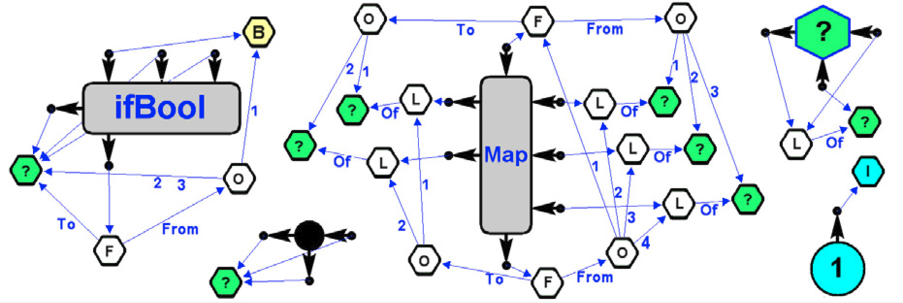
\includegraphics[width=1.000\linewidth]{images/image16.png}
  \caption{The analytics viewer, showing an example stream from the web application.}
\end{figure}

The custom event streams stored by the analytics platform can be viewed in an analytics viewer. To keep the implementation consistent between the main project and the analytics sub-project, it is written as a TypeScript application initialized with Create React App. Using a different framework would have resulted in less knowledge sharing between the two, and introduced additional unwanted complexity. Also, for similar reasons to the main project React was a well-suited framework for the viewer.

The viewer shows analytics events by stream, which can be navigated using the left sidebar which represents a list of streams. The main view shows a list of events within that stream, ordered by timestamp.

\chapter{Implementation}\label{id:h.igepudpadp49}

The application is broken into several loosely-coupled TypeScript modules, as laid out in the design chapter. This chapter details their implementation, examining specific features of the code at a lower level.

\section{Language core}\label{id:h.o3ngfa303saw}

The language core contains models, utility and helper functions, and a lexer and parser. Together these interpret and represent the expression language, and support implementing type inference algorithms upon it.

For clarity, in this section the term `models' will be used to mean TypeScript types, function signatures, interfaces and classes. The term `types' will be used exclusively to refer to the type objects, used for example as the result of type inference algorithms. For example the TypeScript expression in the implementation:

\begin{minted}[breaklines]{typescript}
new TypeVar('t0')
\end{minted}
instantiates a \mintinline{text}{TypeVar} \textit{model} that represents the \textit{type} $t_0$.

\subsection{Models}\label{id:h.f0aymht9bwx3}

TypeScript models are used to represent abstract syntax trees, types, contexts, substitutions, results and errors.

\subsubsection{Abstract syntax trees}\label{id:h.26q0jf334v10}

Abstract syntax trees can be represented by their nodes alone. Each node corresponds to a subexpression, and contains the relevant information about itself and has references to its direct children. For example, the AST for the expression \mintinline{text}{|$\lambda$|x. not x} may be represented by the node:

{\centering \begin{figure}[h!]
  \centering
  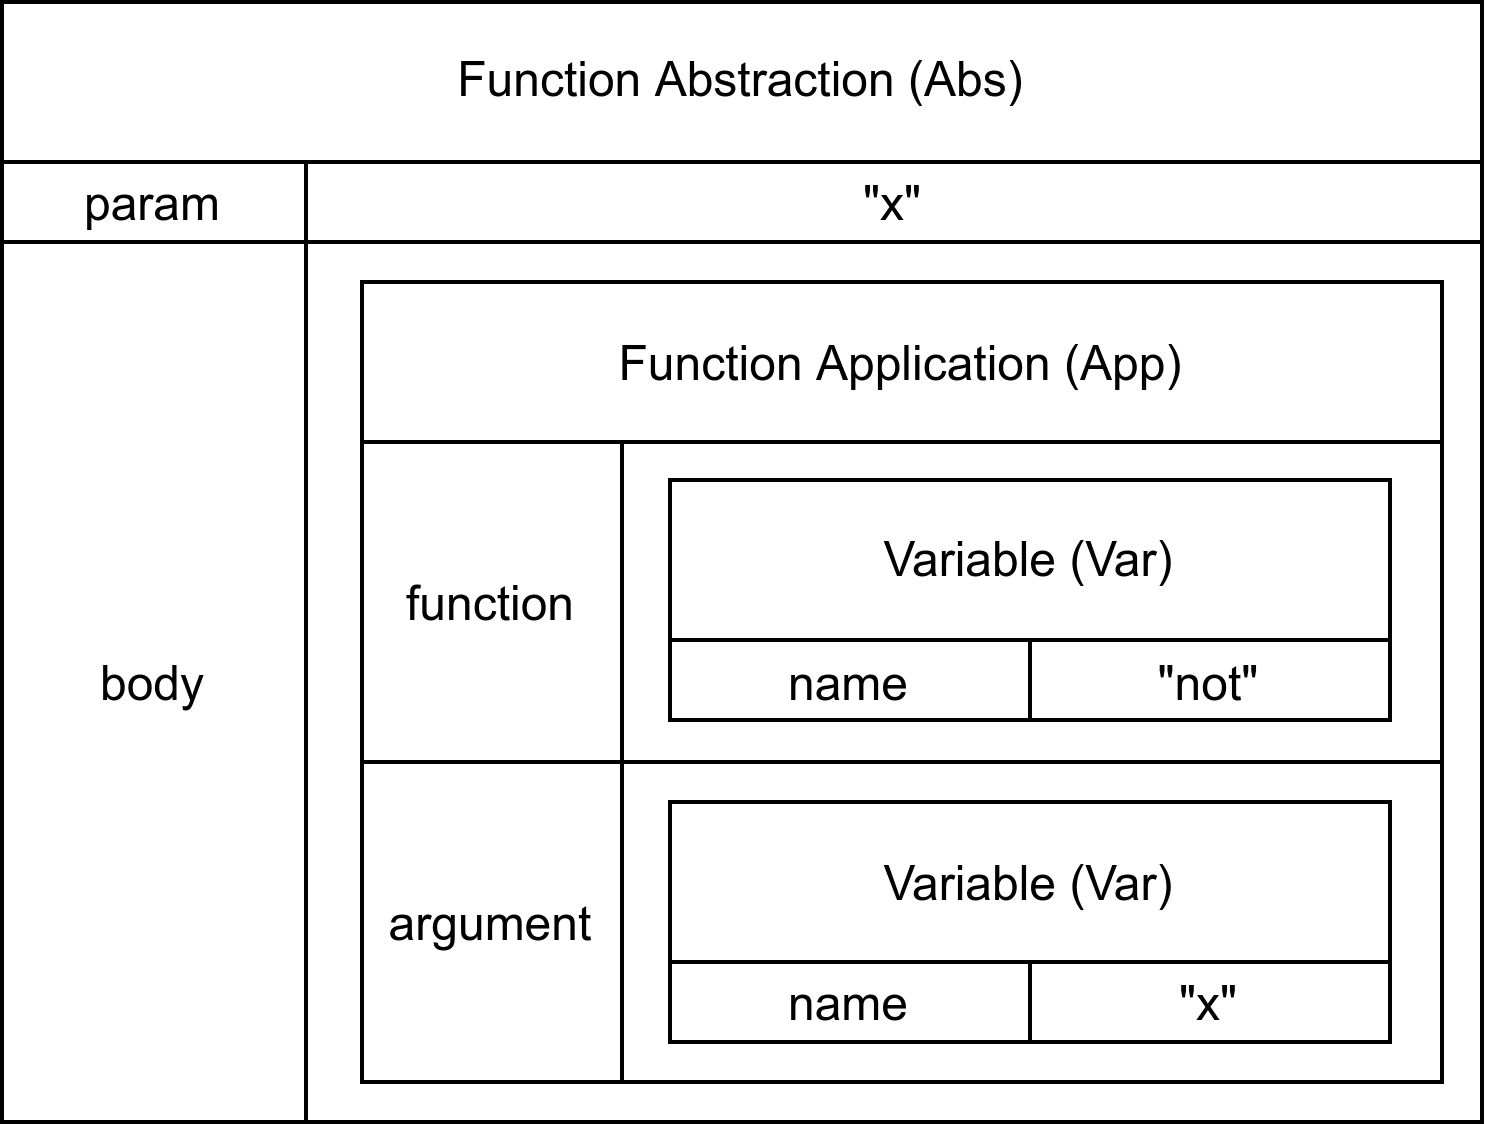
\includegraphics[width=\linewidth]{images/image19.png}
\end{figure} \par}

Here we see the tree is an \mintinline{text}{Abs} node, with a property \mintinline{text}{param} with value `x' and \mintinline{text}{body} property with a reference to an \mintinline{text}{App} node. This \mintinline{text}{App} node has two properties: a \mintinline{text}{function} and \mintinline{text}{argument}, each being \mintinline{text}{Var} AST nodes. These \mintinline{text}{Var} nodes have a single property \mintinline{text}{name}, the name of the variable referenced.

All nodes represent some expression in the original program. We declare a model \mintinline{text}{Expr} as the union of all the different node models, which we can use to represent a general subtree. This is used in defining the node models, for example in its simplest form the \mintinline{text}{Abs} node can be represented:

\begin{minted}[breaklines]{typescript}
interface Abs {
  param: string;
  body: Expr;
}
\end{minted}
To expand upon this, we add the position in the original source program the node was found at. This can be represented by a simple start and end index into the string of the source program, where the start is the index of the first character (0-indexed) and the end is the index of the last character plus one. For example, the \mintinline{text}{Var} node representing \mintinline{text}{not} in \mintinline{text}{|$\lambda$|x. not x} starts at index 6 and ends at index 9. Adding the position of a node helps in debugging, and allows for highlighting the code corresponding to the AST node in the UI on hover.

This indexing scheme is convenient as the length of the expression in the code can be calculated by subtraction, and the standard TypeScript string method \mintinline{text}{slice} uses this convention. Therefore \mintinline{text}{code.slice(p.start, p.end)} results in the source code specified by a position \mintinline{text}{p}.

Positions are represented by the simple model:

\begin{minted}[breaklines]{typescript}
interface Position {
  start: number;
  end: number;
}
\end{minted}
In addition to positions, AST nodes have an optional \mintinline{text}{notes} property that is used to record additional arbitrary information, for example that a node should be highlighted in the UI or that they are from certain syntactically sugared expressions. Notes are represented as an optional string property.

For \mintinline{text}{Abs}, we now have:

\begin{minted}[breaklines]{typescript}
interface Abs {
  param: string;
  body: Expr;
  pos: Position;
  notes?: string;
}
\end{minted}
Once constructed, properties should be immutable. Immutability prevents properties from being changed, which eliminates some hard-to-detect bugs as all object transformations must be explicit. For example, a method call to an object may not unexpectedly change that object. While immutability may have a small performance and memory usage overhead in some implementations, this may be offset (and in some cases, performance may be improved) by structural sharing. Structural sharing uses existing references to parts of an object when making a slightly changed copy of it. This reduces memory usage and reduces the overhead of creating new objects. This can be done safely given the knowledge objects are immutable as neither reference will attempt to update the child. For example:

TODO: diagram

Finally, immutability can improve performance when using front-end frameworks like React, which is used to implement the web application. With immutability, front-end frameworks can be sure objects have not changed on subsequent renders if they have referential equality (they point to the same object). Without immutability, objects may have changed between render calls so the front-end framework must re-render the page or perform deep value equality comparisons which require traversing the entire object. These are both potentially costly operations, so avoiding them through immutability brings performance benefits.

Given the benefits of immutability, models are updated to generally be immutable, marked with the \mintinline{text}{readonly} modifier in TypeScript:

\begin{minted}[breaklines]{typescript}
interface Abs {
  readonly param: string;
  readonly body: Expr;
  readonly pos: Position;
  readonly notes?: string;
}
\end{minted}
As well as the use of \mintinline{text}{readonly} properties on class properties, the keyword \mintinline{text}{const} is preferred to \mintinline{text}{let} or \mintinline{text}{var} when declaring variables. The \mintinline{text}{const} keyword ensures variables are immutable and cannot be redefined (although by itself does not prevent their properties from being modified). The \mintinline{text}{let} keyword in TypeScript allows variables to be redefined, while \mintinline{text}{var} allows variables to be redefined and overwrites them in the global scope which can be particularly dangerous.

To make constructing models easier, we implement these TypeScript interfaces as classes. This allows us to use the \mintinline{text}{new} keyword to construct instances of these models, and we can use the \mintinline{text}{instanceof} operator to verify an AST node is of a specific type more easily. These are not possible with interfaces alone.

In addition, classes allow us to easily add default methods to objects. We add a \mintinline{text}{toString} method to all AST node classes which returns a string containing a program representing the node. This then gives us the final implementation for our \mintinline{text}{Abs} node:

\begin{minted}[breaklines]{typescript}
class Abs {
  readonly param: string;
  readonly body: Expr;
  readonly pos: Position;
  readonly notes?: string;

  constructor(param: string, body: Expr, pos: Position, notes?: string) {
    this.param = param;
    this.body = body;
    this.pos = pos;
    this.notes = notes;
  }

  toString(): string {
    return `(l${this.param}. ${this.body.toString()})`
  }
}
\end{minted}

This structure is used for all the AST node models, including:
\begin{itemize}
  \item \mintinline{text}{Var} for variables
  \item \mintinline{text}{App} for function application
  \item \mintinline{text}{Abs} for function abstraction, as shown above
  \item \mintinline{text}{Let} for let statements
  \item \mintinline{text}{CharLiteral} and \mintinline{text}{NumberLiteral} for literal constants
\end{itemize}

\subsubsection{Types}\label{id:h.bzdo56ibho4h}

As discussed in the background chapter, monotypes are constructed from type variables and type function applications. We consider basic types (such as $Bool$ or $Int$) to be type function applications on zero arguments. Polytypes are monotypes with zero or more for-all quantifier variables.

For simplicity when modelling polytypes, we consider type variables bound at the highest level. Any type that can be expressed with for-all quantifiers at lower levels, is equivalent to moving those bindings to the top level. For example, $\forall a.\ (a \rightarrow (\forall b.\ (b \rightarrow (a,\ b)))$ is equivalent to $\forall a \forall b.\ (a \rightarrow b \rightarrow (a,\ b))$.

Following the same reasoning about using classes with readonly properties we can develop simple models for types. Here we hide \mintinline{text}{constructor} and \mintinline{text}{toString} methods for simplicity.

\begin{minted}[breaklines]{typescript}
type MonoType = TypeVar | TypeFuncApp;

class TypeVar {
  readonly name: string;

  /* constructor and toString methods */
}

type TypeFunc = "->" | "[]" | "Maybe" | "Either" | "Int" | "Char" | "Bool" | "," | ",," | /* ... */;

class TypeFuncApp {
  readonly constructorName: TypeFunc;
  readonly args: MonoType[];

  /* constructor and toString methods */
}

class PolyType {
  readonly quantifiedVars: string[];
  readonly monoType: MonoType;

  /* constructor and toString methods */
}
\end{minted}
\mintinline{text}{PolyType}'s \mintinline{text}{quantifiedVars} property could be modelled with \mintinline{text}{TypeVar[]}, however for simplicity \mintinline{text}{string[]} was chosen as the methods on these type variables are never called.

The constructors are all trivial, and simply set the corresponding properties in the object. The \mintinline{text}{toString} methods are fairly simple for \mintinline{text}{TypeVar} and \mintinline{text}{PolyType}, however \mintinline{text}{TypeFuncApp} has additional logic to pretty-format some types. For example it outputs types like $[(Bool,\ Int)] \rightarrow Int$, rather than $\rightarrow ([]\ (,\ (Bool)\ (Int)))\ (Int)$ which would be the result if it treated all type functions equivalently in prefix notation with explicit bracketing.

\subsubsection{Contexts and substitutions}\label{id:h.ux3btyb2wvh8}

A context, as defined in the background chapter, is a mapping from variable names to their corresponding types. This informs the type inference algorithm what variables are in scope, and what their types are.

Contexts are modelled in TypeScript as objects which have string keys (variable names) and type values. Specifically these type values are polytypes, because as stated before monotypes can be considered polytypes with zero for-all quantified variables. This is written:

\begin{minted}[breaklines]{typescript}
interface Context { [name: string]: PolyType }
\end{minted}
Substitutions can be seen as mappings from type variable names to corresponding types they should be substituted with. In Hindley-Milner there is no need to ever substitute type variables with polytypes, so we can assume these are only monotypes. This therefore can be represented with a model similar to contexts:

\begin{minted}[breaklines]{typescript}
interface Substitution { [name: string]: MonoType }
\end{minted}

\subsubsection{Results and errors}\label{id:h.5yk2zijb0axq}

The parser and type inference algorithms use response models to return their results. A \mintinline{text}{Response} from one of these methods may either be a \mintinline{text}{Rejected} or \mintinline{text}{Accepted}, indicating the input was invalid or valid respectively.

For example, if a syntax error is present in the program passed to the parser, it may return a \mintinline{text}{Rejected} model with the location of the error and a message explaining the issue. Alternatively if a valid program is passed to the parser, it returns an \mintinline{text}{Accepted} model with the AST representation as its value. The type inference algorithms similarly return \mintinline{text}{Rejected} if type inference fails, and \mintinline{text}{Accepted} if it succeeds.

These models are defined:

\begin{minted}[breaklines]{typescript}
type Response<A, R> = Accepted<A> | Rejected<R>;

interface Rejected<T> {
  value?: T;
  accepted: false;
  issuePosition: Position;
  message: string;
}

interface Accepted<T> {
  value: T;
  accepted: true;
}
\end{minted}

These models have generic parameters to specify the type of value expected to be returned. For example, an \mintinline{text}{Response<Expr, ParseError>} represents a model which may either be an \mintinline{text}{Accepted<Expr>}, containing an \mintinline{text}{Expr} as a value, or a \mintinline{text}{Rejected<ParseError>}, containing an optional \mintinline{text}{ParseError}.

In addition to this, a \mintinline{text}{TypeResult} container is defined which is used as part of the function signature for type inference algorithms. This contains a type, representing the overall type of the expression, and the steps the type inference algorithm took to derive that type. Each step has a message and AST to go with it, to match the designed user interface steps.

\begin{minted}[breaklines]{typescript}
interface TypeResult {
  type: MonoType;
  steps: { message: string, ast: Expr }[];
}
\end{minted}

Type inference algorithms return a \mintinline{text}{Response} where if \mintinline{text}{Accepted}, the value should be a \mintinline{text}{TypeResult} object. If \mintinline{text}{Rejected}, the value should be the steps only in the \mintinline{text}{TypeResult}. A TypeScript utility, \mintinline{text}{Omit} is used to remove the \mintinline{text}{type} property from the TypeResult in the rejection case. This gives the overall return type for type inference algorithms:

\begin{minted}[breaklines]{typescript}
Response<TypeResult, Omit<TypeResult, 'type'>>
\end{minted}
In addition to these result wrappers, the parser and type inference algorithms also offer an alternative simple interface which returns just the AST or type. Here if an error is found with the input a \mintinline{text}{ParseError} or \mintinline{text}{TypeInferenceError} is raised, which should be caught by the caller. These errors are also used internally by the methods returning result wrappers.

\subsection{Helper functions and type utilities}\label{id:h.sw77qek8b49p}

Several functions in the language core are relevant to the parser and inference algorithms. Many have already been defined in the background chapter.

\begin{itemize}
  \item \mintinline{text}{|apply|} applies a substitution to a type or context
  \item \mintinline{text}{|combine|} combines substitutions
  \item \mintinline{text}{|unify|} attempts to find a unifying substitution given two monotypes
  \item \mintinline{text}{|contains|} returns whether a type contains a certain type variable
  \item \mintinline{text}{|freeVars|} returns an array of free variables names in a given type or context
  \item \mintinline{text}{|inst|} instantiates a type, replacing all for-all quantified type variables with new type variables
  \item \mintinline{text}{|generalise|} fully generalises a type, for-all quantifying any free type variables in the type that are not free in the given context
  \item \mintinline{text}{|unique|} removes duplicate elements from an array
  \item \mintinline{text}{|diff|} performs the list difference operation
\end{itemize}

Generally the helper functions are written recursively, often with the base case being the when the function is called with a \mintinline{text}{TypeVar} or a \mintinline{text}{TypeFuncApp} with no arguments. This keeps function implementations simple and maintainable.

In addition to these helper functions, there are utilities for constructing types. For example, the type $[Bool] \rightarrow Char$ can be constructed with the classes explicitly:

\begin{minted}[breaklines]{typescript}
new TypeFuncApp('->', new TypeFuncApp('[]', new TypeFuncApp('Bool')), new TypeFuncApp('Char'));
\end{minted}
but with the type utilities, this can be written:

\begin{minted}[breaklines]{typescript}
f(list(boolean), char)
\end{minted}
These type utilities make developing tests significantly easier, and improve readability of the code.

As the helper functions and type utilities are widely-used it is critical that their correctness can be depended upon. To verify correctness, many automated unit tests are run against them using the Jest framework. Jest is a flexible test runner and is recommended by the authors of React for testing React projects. To reduce tooling complexity Jest is used for all automated testing throughout the project.

\subsection{Lexer and Parser}\label{id:h.qbtwwllp8tw6}

The lexer and parser use the Masala library, as explained in the design chapter.

The \mintinline{text}{GenLex} class from the library is used to generate a lexer, which is in turn used for lexing. An instance of \mintinline{text}{GenLex} is used to define different tokens, such as identifiers, parentheses, numeric literals and keywords such as `let'. For example, the left parenthesis token is defined:

\begin{minted}[breaklines]{typescript}
const lparen = genlex.tokenize(C.char('('), 'lparen');
\end{minted}
Once the input program is split into tokens, the parser can attempt to construct an AST. Masala is a parser combinator library, which means functions are chained to parse the expression, each consuming a part of the input.

The parser starts by trying to parse the given program as one of many types of node, using Masala’s \mintinline{text}{|F.try|} utility. This tries to parse the expression with several different construct-specific parsers, taking the first valid match.

These construct-specific parsers match the basic constant, variable, function abstraction and let statement expressions. In addition, we add parsers for tuples and lists that support sugared syntax to allow users to construct these easily. This syntax is similar to Haskell's for lists and tuples. For example \mintinline{text}{[1, 2, 3]} can be specified instead of \mintinline{text}{cons 1 (cons 2 (cons 3 [])} and \mintinline{text}{(1, True)} can be written instead of \mintinline{text}{(,) 1 True}. Lastly, we add a parser for parenthesized expressions to allow making the order of operations explicit.

Once we match one of these parsers, we use it to construct an AST node. Each construct-specific parser returns a single \mintinline{text}{Expr}, and so implements the Masala's TypeScript interface \mintinline{text}{SingleParser<Expr>}. Generally each construct-specific parser extracts the value from the matched tokens, and extracts the location of the node in the source program from a parser metadata object from Masala. The original Masala library does not provide the absolute offset in the source program consistently for all tokens through this metadata object. As Masala is an open-source library, it can be forked and modified. The library was modified to provide the metadata object consistently, and this fork is used in the implementation to get the position property for AST nodes. For example, the rule for parsing and extracting details about a \mintinline{text}{Var} node is:

\begin{minted}[breaklines]{typescript}
const VAR = () => identifier.map((value, r) => new Var(value, getPos(r)));
\end{minted}
(\mintinline{text}{getPos} is a helper function which extracts the token position from the Masala response metadata object \mintinline{text}{r})

More complicated rules such as for \mintinline{text}{|Abs|} use Masala’s tuple model, which collects multiple values and allows accessing them by index:

\begin{minted}[breaklines]{typescript}
const ABS = () =>
  backslash.map((v, r) => r.location() - 1) // store start index
  .then(identifier) // parameter
  .then(arrow.drop()) // dropped as we don’t need info from it
  .then(F.lazy(expression)) // body, F.lazy avoids infinite loop
  // tuple now is (startLocation, parameterName, bodyExpr)
  .map((tuple, r) => new Abs(tuple.at(1), tuple.at(2), { start: tuple.at(0), end: r.location() }))
\end{minted}
At the end of the construct-specific parsers, in the main parser we then call \mintinline{text}{.rep().array().map(nestLeft)}. Together, these handle function application:
\begin{itemize}
  \item \mintinline{text}{.rep()} tells the parser to require one or more construct-specific parsers (similar to the $+$ symbol in common regular expression syntax). This matches function application, as it matches subexpressions separated by whitespaces.
  \item \mintinline{text}{.array()} tells the parser to map these one or more construct-specific parser results into an array (which will result in an array of \mintinline{text}{Expr}s).
  \item \mintinline{text}{.map(nestLeft)} maps the resultant array through the helper function \mintinline{text}{nestLeft}. This \mintinline{text}{nestLeft} function reduces a given array of expressions into an \mintinline{text}{App} model, nesting towards the left as is convention for function application. For example, the array of expressions \mintinline{text}{[a, b, c, d]} would be transformed to \mintinline{text}{App} nodes representing applying the functions in the order \mintinline{text}{((a b) c) d}. In the case only one expression is passed to \mintinline{text}{nestLeft} (i.e., there is not a function application) it simply returns the provided expression.
\end{itemize}

The overall lexer and parser is then wrapped in a function that maps results from the Masala library into consistent \mintinline{text}{Response} models. The wrapper also handles pre-processing the code before passing it to the lexer, and eliminates some special cases to do with disambiguating let-statement related keywords and identifiers.

The parser has many tests, verifying both that valid expressions are parsed correctly and invalid expressions are rejected. Assertions are made on the correctness of parse results, ensuring they return the corresponding AST for the program with nodes being given the expected properties, including their positions.

\section{Type inference algorithms}\label{id:h.flyu66glh76t}

The three type algorithms \W, \W’ and \M\ are implemented in separate packages, as per the design chapter. While by their nature they have differing rules, they all follow a similar overall structure.

Each algorithm exposes a simple public interface, just one method: \mintinline{text}{infer}. This is a polymorphic function which has two possible type signatures. It takes an AST, and an optional boolean toggle to return a \mintinline{text}{Response} model and a custom \mintinline{text}{Context}. If the boolean toggle is false, just a \mintinline{text}{Monotype}is returned. If the toggle is true, a \mintinline{text}{Response<TypeResult, Omit<TypeResult, 'type'>>} is instead returned which represents either a typing result if successful (steps and a final type), or a typing result without a type if unsuccessful (just the steps up to the type error).

This \mintinline{text}{infer} method is a wrapper around the real internal \mintinline{text}{_infer} method, which has a type signature closer to the formal definition of each algorithm. This internal \mintinline{text}{_infer} function is used for recursive calls. When compared to the formal algorithm definitions, The \mintinline{text}{_infer} method has two additional helpers passed in: a fresh type name generator and a logger.

The fresh type name generator yields a new, unused (fresh) type variable name each time it is called. This utility is used to satisfy the requirement for new type variables in the algorithms. Its implementation is simple: it initialises an internal counter to zero, which it returns and increments on each call. For example, subsequent executions might return a sequence of new type variables $t_0$, $t_1$, $t_2$, and so on. This counter is stored in the parent function's scope as a closure to avoid polluting the global state while offering a persistent variable for the duration of the fresh type name generator's lifetime.

The logger records steps the algorithm has taken, in order to display them to the user later. The algorithm calls the logger at each major step, with a dynamic message explaining in context what actions it has performed. In addition, we pass in a map of AST nodes to notes to be applied to the AST corresponding to the step. For example:

\begin{minted}[breaklines]{typescript}
logger('We know the primitive `' + expr.toString() + '` is an `Int`', highlight(expr));
\end{minted}

Results in adding a step with the corresponding message. In the message, backticks are used to represent content that should be shown in monospace font, as is standard in Markdown or on most IM platforms such as Slack, Discord and Microsoft Teams. The \mintinline{text}{.toString()} method is one defined as part of the AST node models. The \mintinline{text}{highlight} helper function results in a map, which when passed to the logger adds a note to highlight the given expression in the UI.

The logger's implementation is somewhat similar to the fresh type generator's implementation. Rather than initializing just a counter, we initialize an empty array. Each time the logger is called, it applies the notes to a clone of the AST and pushes a step into the array. At the end of the type inference process, the steps array is extracted and returned as part of the result to the caller of the \mintinline{text}{infer} method.

In the internal \mintinline{text}{_infer} method, generally we are given an AST node which we can match against the different classes. Each different class of AST node has its corresponding rule in the algorithm implemented using the helper functions from the language core. For example, for function abstraction in algorithm \W\ the rule:
\begin{align*}
\mathcal{W}(\Gamma,\ \lambda x.\ e  ) =\ & \textrm{let}\ (S_1,\ \tau_1) = \mathcal{W}(\Gamma + x : t_0, e),\ \textrm{new}\ t_0\\
& \textrm{in}\ (S_1,\ S_1(t_0 \rightarrow \tau_1))
\end{align*}

can now be directly implemented in TypeScript as:

\begin{minted}[breaklines,escapeinside=||]{typescript}
if (expr instanceof Abs) {
  const |$\beta$| = new TypeVar(freshTypeName());
  const [S1, |$\tau$|1] = W(e, { ...|$\Gamma$|, [x]: pt([], |$\beta$|) });
  return [S1, apply(S1, f(|$\beta$|, |$\tau$|1))]
}
\end{minted}
While the actual implementation differs slightly from this (adding logger calls, using different variable names and passing down the helpers recursively) the structure is the same. Further rules and other algorithms are implemented similarly, again with minor tweaks to the algorithms to catch type-errors and log the steps taken.

This implementation of the type inference algorithms as standalone functions to be applied to AST nodes is the result of several iterations of development. While appearing simple, getting the models right to represent the algorithms elegantly in TypeScript was a significant challenge.

An initial implementation extended the AST node classes with type metadata, helper functions and inference methods. The inference algorithms then would map ASTs to these extended models and call the inference method on the root node. However, this strategy resulted in a lot of code duplication (especially in helper methods) and was difficult to test. In addition, debugging problems was difficult as it was tougher to follow the call stack in the class methods. Finally, the significant difference between a class-based implementation and the way the algorithms are commonly presented made spotting deviations from the algorithms specifications difficult.

A later implementation moved closer to the current implementation but inlined many of the simpler helper functions. This was slightly more performant than the final implementation, however, inlined functions reduced code readability and removed the ability to unit test helper functions on their own. While closer to the formal algorithm specifications, it did make detecting differences between the implementation and the specification harder.

As the inference algorithms implement the same interface they can share high level tests, as we expect the same result from each of them. A comprehensive test suite is packaged alongside the implementation, covering a range of expressions and edge cases, including incorrectly-typed expressions. To help with this, custom assertion matchers were added to the testing framework.

{\centering \begin{figure}[h!]
  \centering
  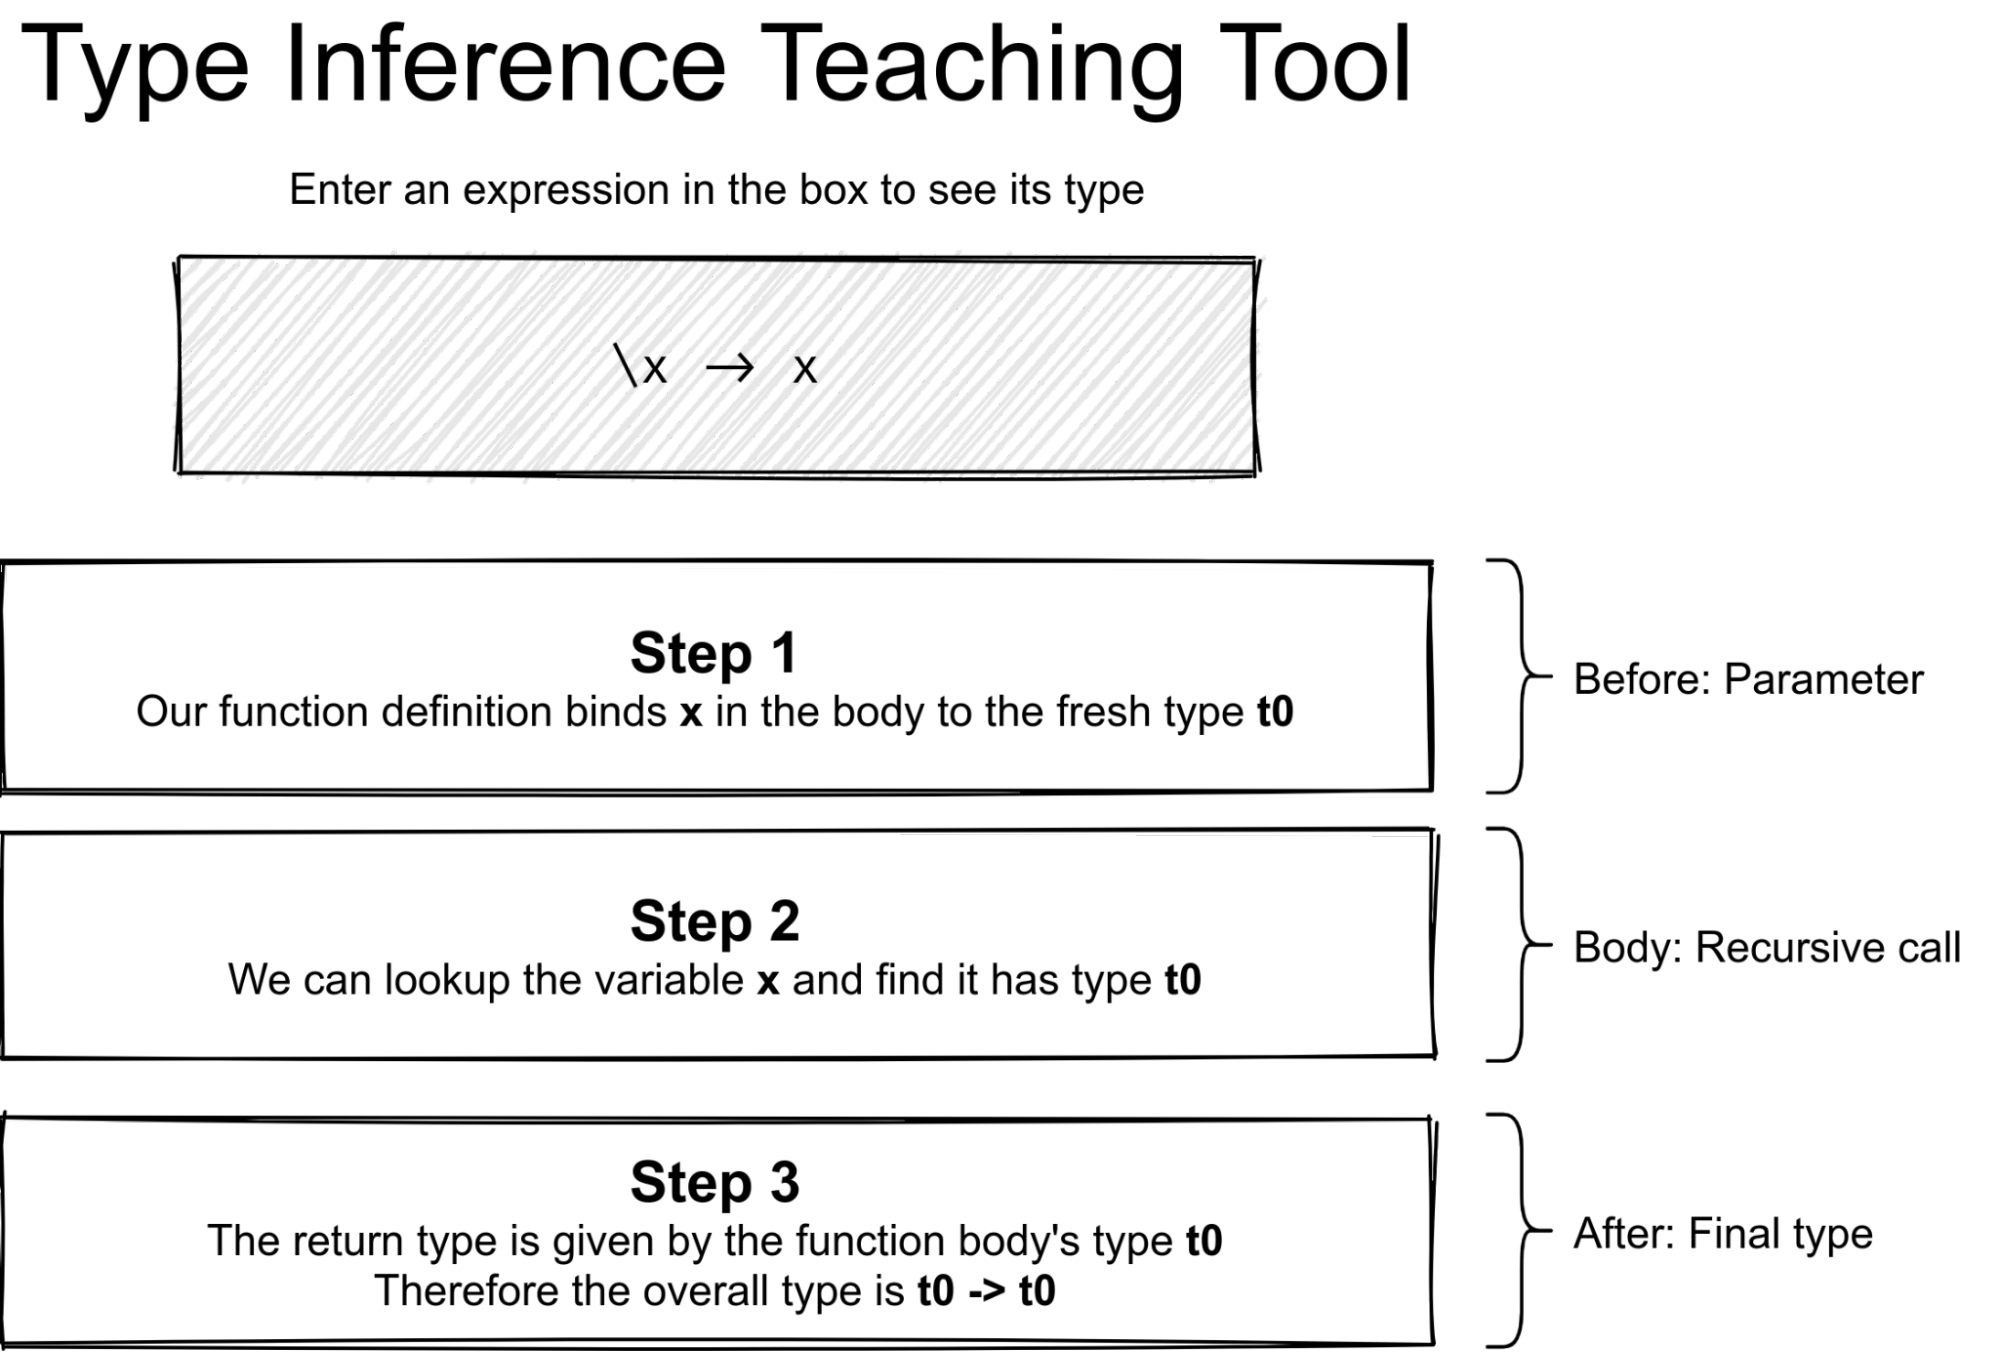
\includegraphics[width=0.769\linewidth]{images/image9.png}
  \caption{Example test framework output to the command line showing a failing custom assertion}
\end{figure} \par}

The first custom assertion matcher, \mintinline{text}{expect(expr).toHaveType(type)} asserts that when the type inference algorithm is applied to the given expression \mintinline{text}{expr}, the type \mintinline{text}{type} is returned. This matcher uses a custom deep equality check on types, allowing for $\alpha$-equivalence (type variables to be renamed consistently throughout the type). For example, the types $t0 \rightarrow Int$ and $t1 \rightarrow Int$ would be considered to be equivalent by renaming. Note that a pair of types being $\alpha$-equivalent is different to being unifiable as the types must still have the same structure, just the variable names can be changed between them.

The second assertion matcher, \mintinline{text}{expect(expr).toHaveInvalidType()} asserts that the type inference algorithm raises a type error when applied to the expression \mintinline{text}{expr}.

Both assertion matchers pretty-print output on failure, clearly highlighting where the resultant types differ. They also both support negation, for example \mintinline{text}{expect(expr).not.toHaveType(type)} asserts that an expression is not given a certain type by the type inference algorithm.

\section{Web application}\label{id:h.jqmg1n3w35mp}

The React web application is composed of several reusable components. These components are managed by React, which injects the \mintinline{text}{Main} component as the root node of the application.

This \mintinline{text}{Main} component is responsible for rendering most of the application, through creating child components and managing the state used to configure the user's input (such as the algorithm selected and the program entered).

State in the application is managed with React hooks, and the components in the application are written as functions. This is the currently recommended way to develop React applications, as opposed to using older-style class components. React functional components with hooks are less error-prone and are easier to use than class components. In addition, generating and passing around callbacks to update state is significantly easier with hooks. This is used in the application to power reusable components such as the \mintinline{text}{SetButton} component, which takes a setter callback and triggers it when the button is clicked.

A key component is the \mintinline{text}{ResultView}, which displays the result of running the type inference algorithm on the user input. It is this component which also calls the parser and type inference algorithm to get the result, and displays any errors if the input is invalid. It in turn calls the \mintinline{text}{ASTView} to display the AST where relevant.

The \mintinline{text}{ASTView} component constructs a visualisation of a given AST. Like the type inference algorithms, there are cases for each type of AST node which may recursively display parts of that node. The \mintinline{text}{NodeView} displays a complete AST node, recursively calling itself, \mintinline{text}{NodeWrapperView} and \mintinline{text}{NodeChildView}. \mintinline{text}{NodeWrapperView} represents a horizontal bar in the AST, wrapping some text content. \mintinline{text}{NodeChildView} adds a level indentation so children appear further to the right than their parents. Together, along with some CSS pseudo-elements they are styled to add lines between parent and child nodes. This implements the design of the AST laid out in the design chapter.

{\centering \begin{figure}[h!]
  \centering
  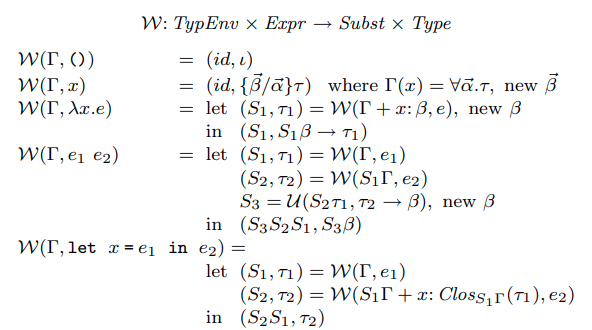
\includegraphics[width=0.814\linewidth]{images/image1.png}
  \caption{Example visualisation of an AST by the ASTView}
\end{figure} \par}

TODO: annotate the diagram above

The \mintinline{text}{|ASTView|} takes a callback function, which is triggered when an AST node is hovered over. It is passed the AST node’s corresponding position in the input program, which is used to highlight that part of the input.

{\centering \begin{figure}[h!]
  \centering
  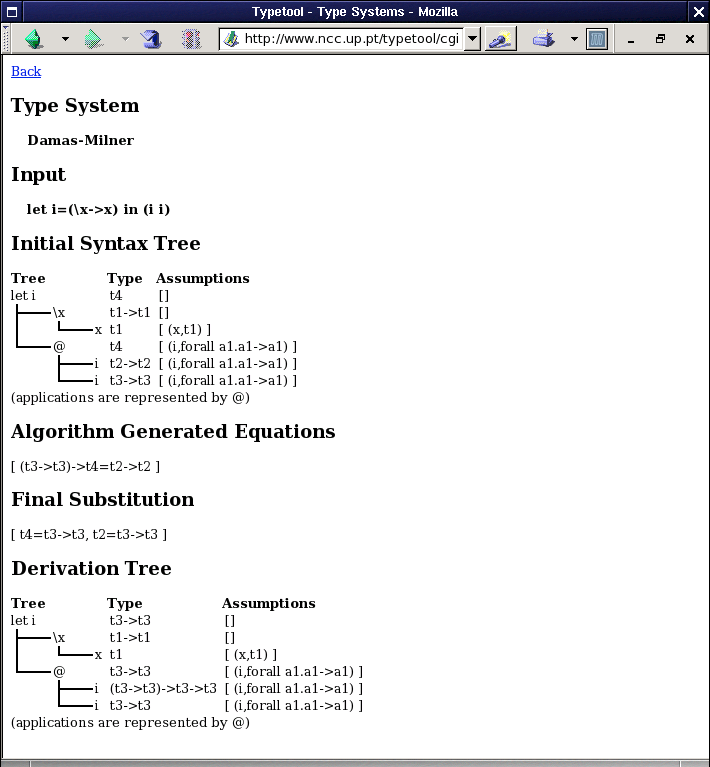
\includegraphics[width=0.868\linewidth]{images/image2.png}
  \caption{The second function application node is hovered here, highlighting the 'map not' part of the expression.}
\end{figure} \par}

TODO: add cursor position to above screenshot

To improve the performance of the web application, the \mintinline{text}{Main} component memoises renders of \mintinline{text}{ResultView}. This means that on future renders of the \mintinline{text}{Main} component, the \mintinline{text}{ResultView} is only re-rendered (and thus the parser and type inference algorithms are only re-run) if the input expression or the selected algorithm changes. This avoids unnecessary computation when other state in the \mintinline{text}{Main} component changes, for example when the user opens the help window, this updates the \mintinline{text}{Main} component's state but does not cause the \mintinline{text}{ResultView} to re-render.

TODO: show performance flamegraph/render latency comparison with and without useMemo

The help window explains the language's type constructors and lists the available variables in the global context. It is implemented as a modal that can be toggled with a button, and can be scrolled independently of the main page. The documentation on the available variables is automatically generated from the context, using the language core's helper functions and its model's \mintinline{text}{toString} methods.

TODO: screenshot of the help window

The web application also uses the Jest framework for testing. In addition, it uses the React Testing Library to simulate browser events, such as clicking buttons and entering text into the input box. Some of these tests are effectively end-to-end tests as they simulate a certain user journey. Some may also be considered integration tests, as assertions are made on the behaviour of the web application in combination with the language core and type inference algorithms, ensuring all the modules work correctly together.

\section{Analytics}\label{id:h.39bhrrv1fi5p}

Recording analytics is built into the web application, which makes calls to a RESTful HTTP endpoint to record events. This is guarded by a check of the ``Do not track'' browser flag to ensure user's privacy preferences are respected.

On load, a randomised identifier is generated and each subsequent event is sent along with this identifier, which allows them to be viewed in an event stream. However, this identifier does not tie the data to any specific person and is therefore not considered personal data.

The RESTful API offers one simple endpoint which saves valid JSON events sent to it. The API is served by Amazon Web Services (AWS), a cloud platform. First the HTTP request is received by an API gateway, and provided it passes basic security checks it is forwarded onto an AWS Lambda function. The function first checks the data sent to it against a schema and if it is valid the event is stored in S3, an object storage service. If the data is invalid, the request is rejected.

Events can then be later retrieved from S3 by authorised users, who can visualise them using the analytics viewer. S3 is configured to automatically delete events after a period of 90 days, to follow best practices on data retention.

These cloud products are all considered `serverless', in that they do not require the explicit management of servers. This reduces running and maintenance costs as the code is only executed when users are using the application. It also improves scalability, as more capacity can automatically be provisioned for the analytics tool to meet user demand.

\chapter{Evaluation}\label{id:h.e6letww4nhn0}

User testing aims to evaluate whether the teaching tool works and is effective in its current form. These aims can be summarised by:
\begin{enumerate}
  \item the tool is accessible and users can enter input
  \item the tool's outputs can be understood
  \item the tool improves students' understanding of types and type inference
\end{enumerate}

From 1 to 3, these increase in scope and in how difficult they are to measure. However, the key aim is 3, as if the tool meets the first two aims but does not improve student understanding it is still not helpful as a teaching resource.

To verify whether the project meets these aims, a questionnaire was distributed to students and analytics data from the web application was reviewed.

\section{Questionnaire}\label{id:h.yqiowsgjmohq}

The questionnaire was composed of three parts: a short test on types and type inference before using the application, introducing users to the application and asking usage questions, then a final test to see if student’s performance improves after using the tool.

This addresses and allows for measurement against all three aims. The tool’s performance on aims 1 and 2 are measured in the middle part, where users are asked to access the tool, enter input and interpret the results. Aim 3 is measured by looking at the relative difference in test results from before and after using the tool.

The questionnaire was distributed in several student-organised group chats and online communication platforms relating to computer science. In addition, my supervisor encouraged students on his CS141 Functional Programming module to complete the questionnaire, highlighting it in lectures and several seminar sessions.

To incentivise students to fill out the questionnaire with detailed and accurate answers, an achievement through the Warwick Automated Assessment Tool (WAAT) was offered to all students who made an honest attempt at all the questions. Student were considered to done this if they selected the correct option for the following quality control check question:

{\centering \begin{figure}[h!]
  \centering
  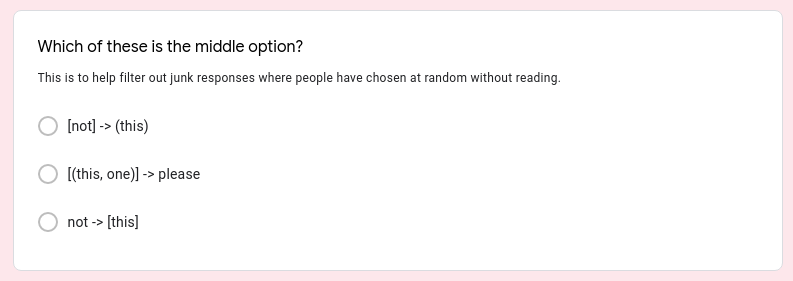
\includegraphics[width=0.9\linewidth]{images/image32.png}
  \caption{The quality-control question to ensure users were reading and answering questions properly}
\end{figure} \par}

In addition to the WAAT achievement, vouchers were given to four random respondents and to two respondents who gave detailed constructive feedback on the tool. Finally, students were also reminded that learning about types and type inference would improve their functional programming skills, which could help them with the CS141 assessments. While students were encouraged to complete the questionnaire, it was made clear that it was optional, it would have no direct effect on any of their assessments and that they could choose to stop taking the questionnaire at any time.

The questionnaire had 48 unique responses, of which 46 were valid (where the respondent had fully completed all questions, and answered the quality control check question correctly). Percentages given here are with respect to the number of valid responses.
\subsection{Direct questions}\label{id:h.abykou9pzwwh}
The second part of the questionnaire asks direct questions about the tool. There are two types of questions in this part. The first type asks users to try accessing the tool, inputting results and interpreting the results. These questions are:
\begin{itemize}
  \item Try entering: \mintinline{text}{map odd []}. Try to understand the steps. What is the unifying substitution performed in step 3?
  \item Try entering: \mintinline{text}{not 3}. Try to understand the steps. What is the problem found?
\end{itemize}
Both of these questions offer 7 multiple choice options, of which only one is correct. These options included the chance to say they could not enter the input, or could not understand the output. In addition, the questions allow users to enter an ‘other’ free-text response.

The first of these questions had 42 (91\%) respondents select the correct answer. 2 respondents chose a type closely related to the substitution but not the substitution itself, and 1 respondent manually entered a different substitution. 1 respondent did not understand the output enough.

The second had all respondents select the correct answer.

In both questions, no respondents selected that they could not access or use the software, and the high correct response rate for both questions provides evidence the tool meets aims 1 and 2.

The second type of question in the second part of the questionnaire seeks feedback on what the tool does well, and how it might be improved upon. These are long-answer text questions with open prompts. This encourages users to be candid in their answers and allows them to comment freely about their experiences with the tool. The questions are:
\begin{itemize}
  \item What is really helpful about this tool?
  \item What could be improved in this tool?
\end{itemize}

These questions give better insight into what helps students understand type inference, so the tool can be improved. Determining what is most helpful about the tool can confirm which parts are working well already, while asking what could be improved highlights areas to be changed.

42 respondents answered the first question. Several of these responses were very thorough, and many themes were mentioned by multiple respondents. These common themes are summarised below:
\begin{itemize}
  \item 23 said the steps are clear / easy-to-understand
  \item 15 said the steps are well-presented / well-visualised
  \item 13 found it helpful for understanding unification
  \item 11 found it helpful for understanding type inference
  \item 9 liked the visual design and colour scheme
  \item 8 liked that the tool explains why invalid expressions are invalid
  \item 8 stated showing substitutions helps explain unification
  \item 4 said the tool helped them better understand Haskell
  \item 2 said function application is explained well
  \item 2 said the tool helps explain curried functions
  \item 1 learnt how let syntax worked
  \item 1 said the tool is most helpful for complex examples
  \item 1 said the application is very fast
\end{itemize}

In addition to these themes, several quotes highlight the positive experiences users had with the tool. One user states the importance of type inference, and the necessity of having a teaching tool for it: “Type inference is hard, and tools to make it easier for people to understand are both helpful and necessary. Thank you!”, and another suggests an interactive tool may be more effective than traditional learning materials: “I think that this type of learning (trial and error) is much more effective than just learning some rules from slides/books.” Students found that “all the steps are shown clearly”, with one saying “I love the level of detail the tool goes to to suggest why type errors may have occurred”.

As well as feedback supporting the explicit aims of the user testing, some responses validated design decisions made in presenting the type inference results. For example on the AST visualisation and highlighting, a user remarks “The tree-type structure that shows how certain steps result from other steps makes it really clear how the process of type checking works, and the colour highlighting makes then shows what step of the process it being worked on at a time.” Another user similarly mentions the AST view, writing “The diagram at the start of each step showing the sort of "graph" of the function inputted helps me visualise the order in which parts of the function need to be "broken down" to get a simpler type overall.” The presentation of unification in the steps of the type inference algorithms was also commented on, with a user stating “Explicitly showing the concept of "unifiable" was very nice, I didn't get that when I did CS141. I understood the concept of "these types kinda fit together" but not exactly why.”

38 respondents answered the second question. Generally respondents were very positive about the tool, and several used this question to continue discussing its benefits. However, the more negative themes and constructive criticisms were:
\begin{itemize}
  \item 5 wanted more general information on the HM type system and the HM algorithm
  \item 4 suggested using arrows to navigate through steps rather than scrolling
  \item 3 suggested improving the wording of the function application step
  \item 2 wanted support for declaring a custom global context
  \item 2 wanted it made clearer that the expression box was a text input
  \item 2 spotted a typo ‘instatiate’ instead of ‘instantiate’
  \item 2 wanted additional information on the homepage
  \item 2 suggested adding animations
  \item 1 wanted the order of the AST and text in a step swapped
  \item 1 wanted contact details on the website could to report bugs and feedback
  \item 1 wanted automatically suggested typo corrections e.g. ‘Fals’ to ‘False’
  \item 1 said that on mobile changing the expression caused the screen to move
  \item 1 requested functor and applicative support
  \item 1 requested support for list comprehensions
  \item 1 suggested adding a quiz mode
  \item 1 wanted their expression to be visible when scrolled down the page
  \item 1 said they disliked colour scheme
  \item 1 wanted more use of mathematical notation
  \item 1 wanted a dark theme
\end{itemize}

Users want more general information on Hindley-Milner and type inference. While they found the tool useful for specific examples, a basic introduction or tutorial could be added to help explain type inference for those completely new to it. For example, a user explains “it would be a good idea to add a section that describes the general process of how it works and then go on to the specific examples”. Another user says the existing information is sufficient, but could be made more prominent with a tutorial page: “The explanation of the tool is robust but could be made more obvious as its [sic] easy to miss. This could be incorporated in the form of a tutorial page perhaps?”

Several users mentioned that they would prefer to click through the steps, rather than scroll through all the output. While similar interactive teaching tools such as WolframAlpha Step-By-Step, Cymath and Khanacademy show steps sequentially for scrolling, these services’ steps are generally shorter so perhaps this pattern is applied differently there. For example, a respondent comments “Output generated is very long and requires a lot of scrolling. If the explanation was layed [sic] out side-by-side with the diagram I feel that would make it easier for someone to parse and a "move to next step" button might save some scroll time.”, and that “Maybe it could be a good idea to have arrows to move between different steps instead of having to scroll down, especially for expressions that have large visualisations”.

While users praised the AST visualisation in the first question, some thought the way function application was shown could be improved, with one suggesting “just showing "Function Application" is a bit opaque, maybe add the function being applied for clarity?”. Some of this feedback may have been due to a misunderstanding of what the “Function application” node represents: it applies the first child (the function) to the second child (the argument). However, this view could potentially be improved by showing the text representing the function being applied in the function application node, or having a function and argument prefix on the child nodes.

Some less commonly raised feedback, for example making it clearer that the expression box was an input and fixing the typo ‘instatiate’ could be directly fixed in the web application. For example, these were fixed by autofocusing and displaying a cursor in the input box, and updating the website copy respectively. Other larger extensions such as adding applicative and functor support (which would require adding typeclasses) or adding a quiz mode would be useful extensions to the project, but due to project time constraints have not been implemented.

\subsection{Test performance}\label{id:h.cn0p90nrqrmi}

The first and third parts of the questionnaire were tests on types and type inference. While the two tests were not identical to avoid commitment bias and choosing the same answers in the tests without revaluating the questions, they were very similar and of equal difficulty. The intention of these tests is to evaluate the tool against aim 3, measured by the difference in performance before and after using the tool. To make the tests easy to fill out and mark without bias, all questions were multiple-choice.

{\centering \begin{figure}[h!]
  \centering
  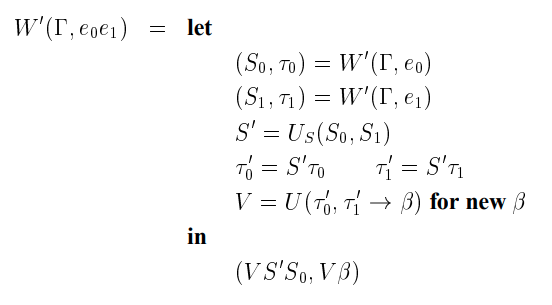
\includegraphics[width=0.9\linewidth]{images/image11.png}
  \caption{An example multiple-choice test question asking about the type of an expression}
\end{figure} \par}

Average test scores improved from 54\% to 69\% after using the tool. This is a statistically significant change at the p < 0.001 level.

Statistical significance is determined using a paired two-sample t-test, a technique where each respondent's before and after test scores are paired up and used to determine how likely the before and after set are drawn from the same population (i.e., that using the tool had no change on their ability). A low p value indicates it is very unlikely they are from the same distribution, so using the teaching tool has had an effect on their ability to choose correct answers to questions on types and type inference. Typically p-values less than 0.05 are considered significant, with lower p-values showing higher significance. t-tests are commonly used in medical and evidence-based education trials to determine whether an intervention makes a difference, where randomised controlled trials are not practical. While a randomised controlled trial may have been preferable (where some users would be given a control of a different, non type-inference related website to view) this would have halved the effective sample size. Given that when producing the questionnaire it was unknown how many participants would answer, it was less risky to run a t-test evaluation.

{\centering \begin{figure}[h!]
  \centering
  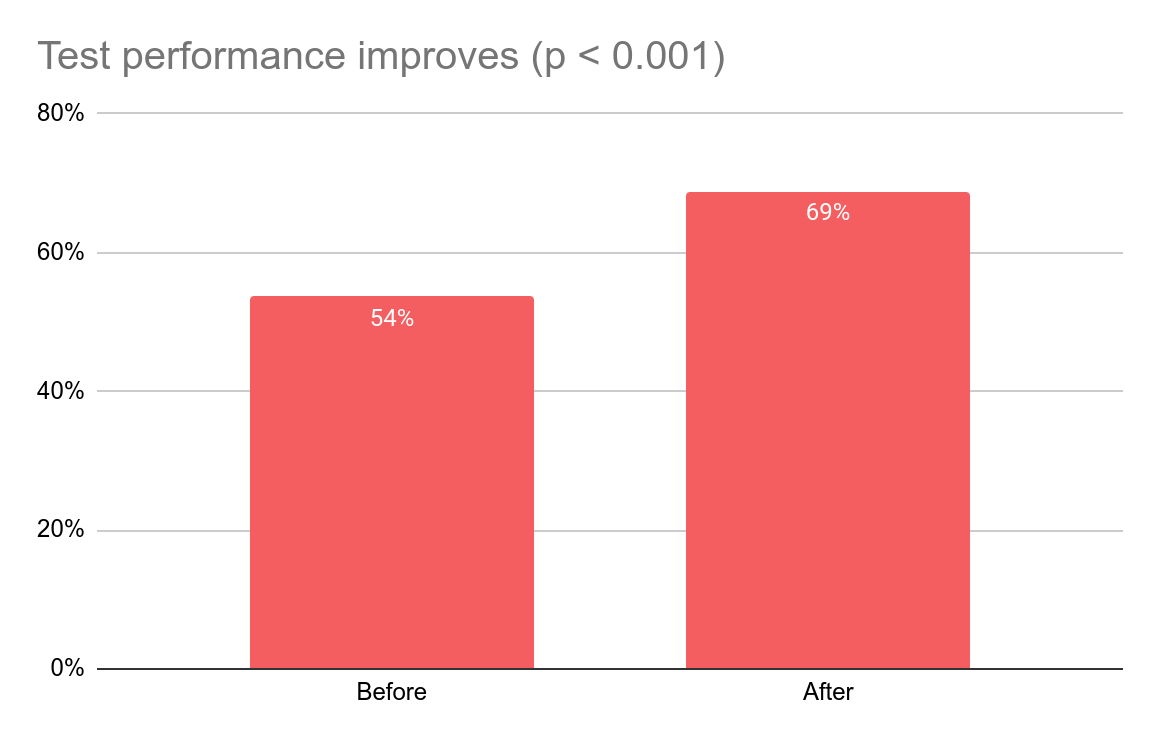
\includegraphics[width=0.85\linewidth]{images/image23.png}
  \label{figure:evaluation_testperformanceimproves}
\end{figure} \par}

In addition to performance improving in general, we can also examine how useful the tool is to users of different abilities. Students with a wide range of abilities answered the questionnaire, as can be seen by the distribution of test scores. This suggests an academically diverse set of students responded to the survey, improving the quality of the results as the responses represent more students than just the current top-performers.

{\centering \begin{figure}[h!]
  \centering
  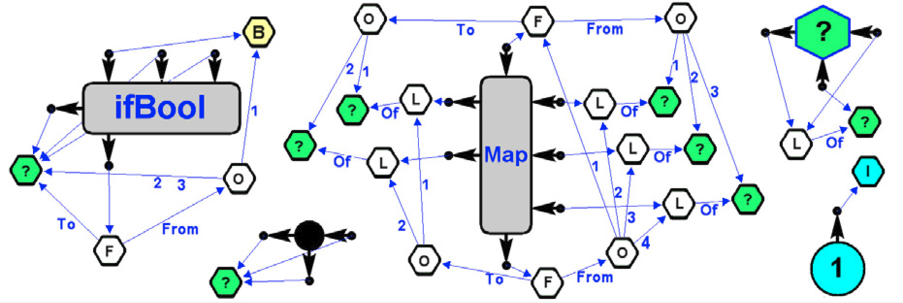
\includegraphics[width=0.9\linewidth]{images/image3.png}
  \label{figure:evaluation_testperformancedistribution}
\end{figure} \par}

We first explore how different quartiles of students perform before and after using the tool. These quartiles are drawn from the student's performance in the `before' test, i.e. Quartile 1 is the bottom 25\% of respondents based on `before' test answers. We see that performance consistently improves for all quartiles, in fact with each quartile's `after' score beating the next quartile's `before' score. This performance improvement is statistically significant for all quartiles. Average performance increases most in quartile 1, as might be expected as these students have the greatest possible improvement possible.

{\centering \begin{figure}[h!]
  \centering
  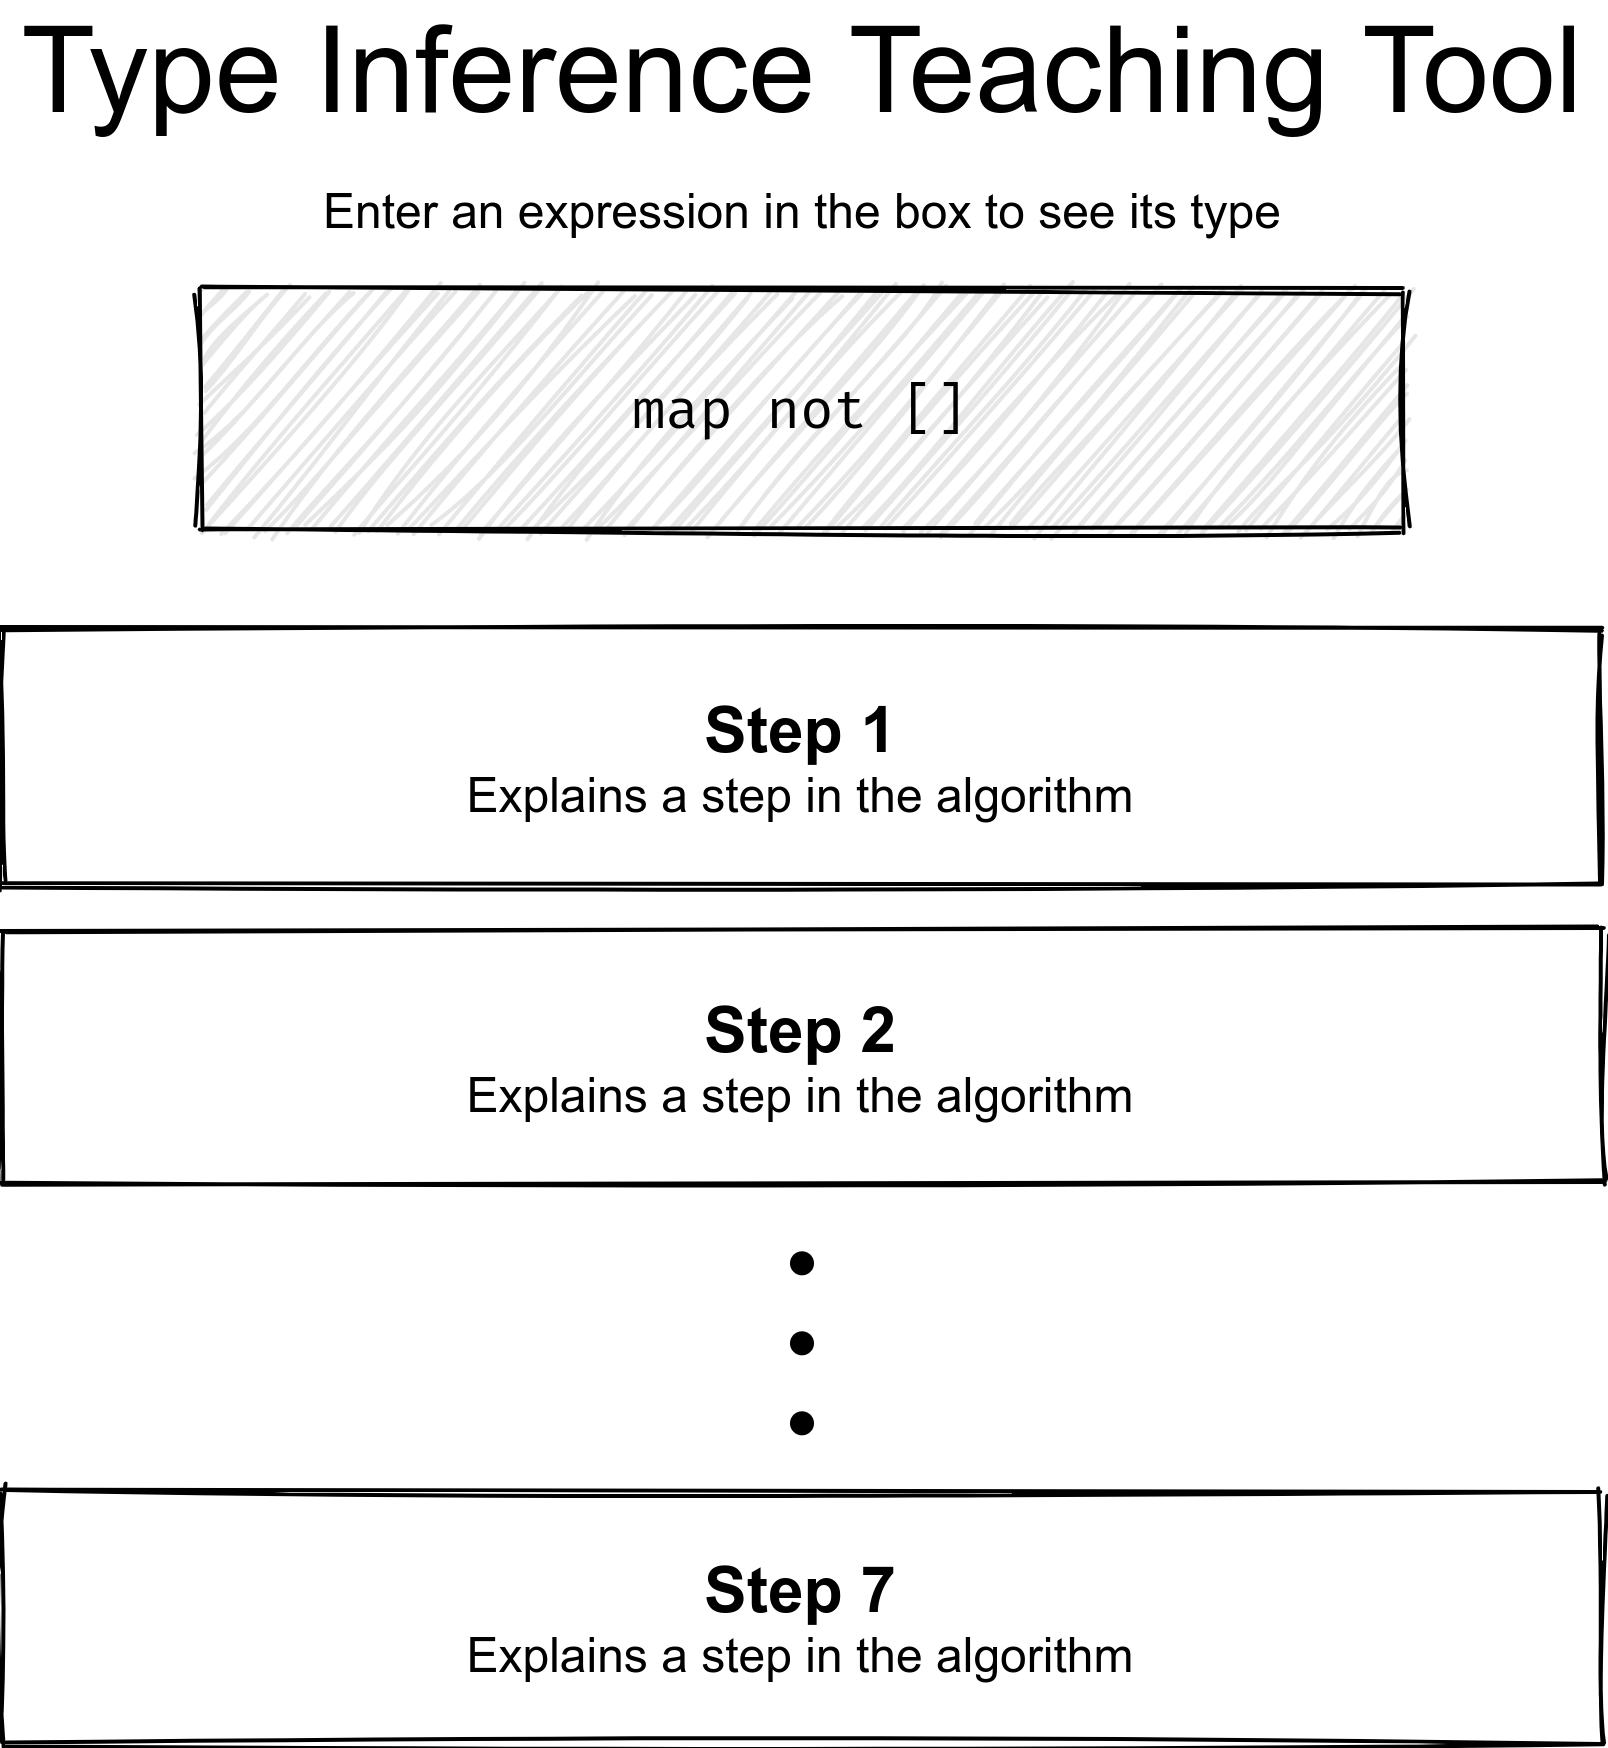
\includegraphics[width=0.85\linewidth]{images/image20.png}
  \label{figure:evaluation_testperformancecohorts}
\end{figure} \par}

At the beginning of the questionnaire, users were also prompted to self-report how well they believed their understanding of types was (``How would you rate your own understanding of types?'') on a 5-point scale from `Very weak' to `Very strong'. No respondents chose ‘Very weak’, and most (27) respondents chose `Average'.

We can also show how performance improves based on these groups. These self-reported groups correlate well with performance, showing students have a somewhat accurate idea of their own ability of understanding types. Again, performance improves for all groups, although this increase is not statistically significant for the `Weak' and `Very strong' groups, likely due to their small sample sizes.

{\centering \begin{figure}[h!]
  \centering
  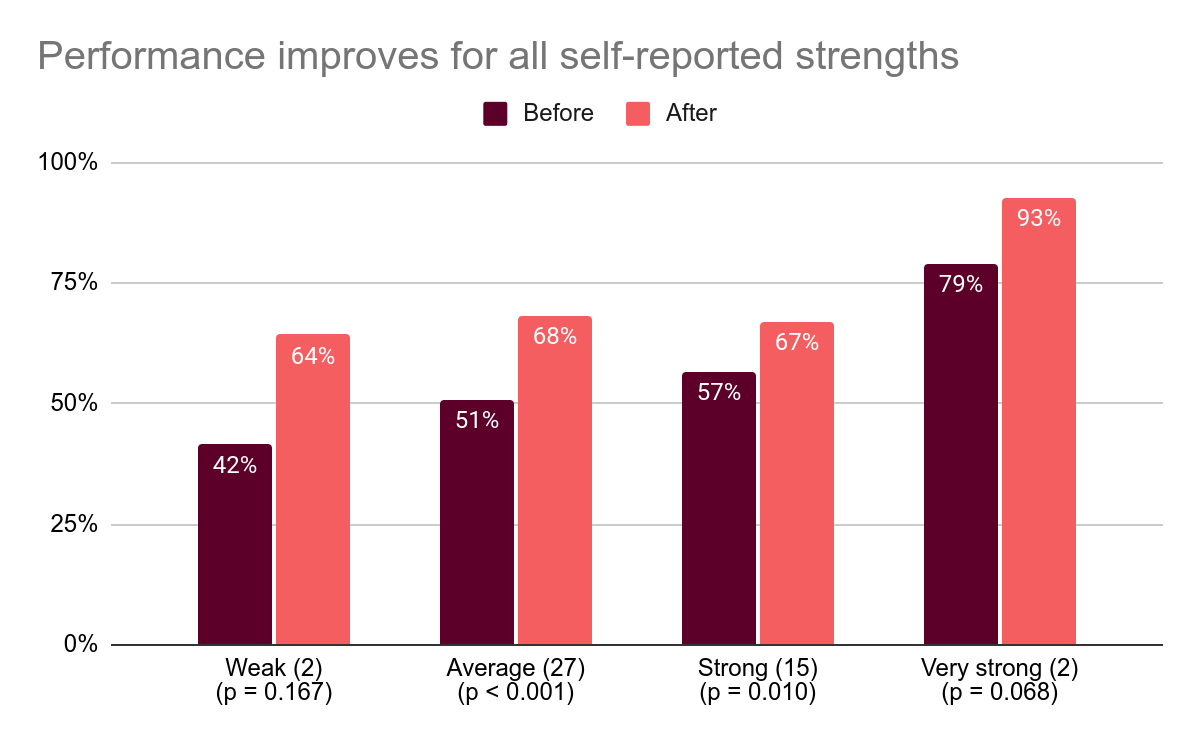
\includegraphics[width=0.85\linewidth]{images/image27.png}
  \label{figure:evaluation_testperformanceselfreported}
\end{figure} \par}

\section{Analytics}\label{id:h.67g05flyfv0z}

Anonymised usage data is collected by the web application. Events recorded include page visits, opening and closing the help section and code expressions entered. To avoid recording testing of the site, my own visits are excluded from the analysis. This data directly verifies aim 1, and provides evidence for the tool achieving aims 2 and 3.

The data shows users are able to access the site and can use the examples and enter in their own expressions, supporting aim 1. This was particularly useful in giving confidence that the site was working correctly while waiting for questionnaire responses to be returned.

Several event streams provide evidence that user understand the results of the type inference algorithms, and can debug their code appropriately to fix errors. This supports aims 2 and 3. This can be seen in an extract from an event stream:
\begin{enumerate}
  \item the user loads the page
  \item the user enters \mintinline{text}{|map od []|} as an expression, which displays a type error as \mintinline{text}{|od|} is not defined
  \item the user corrects this to \mintinline{text}{|map odd []|}
  \item the user builds upon this, adding a list of numbers: \mintinline{text}{|map odd [3]|}
\end{enumerate}

We can also see other users composing more complicated example expressions from the samples for example:
\begin{enumerate}
  \item the user loads the page, and tries several examples
  \item the user tries the \mintinline{text}{map not []} sample
  \item the user tries the \mintinline{text}{let x = 3 in (+, x)} sample
  \item the user tries their own \mintinline{text}{(+) 3 1} expression
  \item the user composes this with the \mintinline{text}{map} example, trying \mintinline{text}{map (+4) int}, which displays a type error as \mintinline{text}{+4} is not a function so is not a valid argument for \mintinline{text}{map}
  \item the user adjusts this to \mintinline{text}{map (+ 4) int}, which displays a different type error saying that \mintinline{text}{int} is not in scope
  \item the user finally corrects the final type error in the expression to get \mintinline{text}{map (+ 4) []}, and the type \mintinline{text}{[Int]} is displayed
  \item the user remains on this derivation for some time, suggesting they read the steps in detail, then clears the input and tries other expressions
\end{enumerate}

All types of analytics events were fired, which suggests all features of the application were used. Most users selected an example expression and entered their own custom expressions. Relatively few users viewed the help window and those that did usually had it open for less than a minute, which supports the criticism found in the questionnaire that the help could be made more obvious and its content could be changed to be more engaging.

\section{Ethics}\label{id:h.q5st3bb4afm1}

Participants safety and privacy was carefully considered during the evaluation of the tool through the questionnaire and analytics data.

The questionnaire was completely entirely online, requiring no face-to-face contact which eliminates the risk of COVID transmission. A questionnaire online also reduces the time investment respondents have to put in and reduces the social commitment of completing it so that participants are less pressured to complete it without feeling fully comfortable. Users were informed that participation was entirely voluntary and that they could discontinue at any time.

The questionnaire minimised personal data captured. Email addresses were the only explicitly personal data requested, and only if the user wanted to receive an achievement and be entered to win a voucher. A support email address was made available in case respondents had questions or concerns, or wished to exercise any of their data rights. No questions or concerns were raised through this.

In addition, as the questionnaire was promoted through the CS141 module, to prevent unintentional undue pressures to complete the survey it was made clear that the questionnaire had no impact on students’ marks, and that before or after test performance would not be shared, and would not be analysed alongside any personal data.

Analytics data is only collected on the type inference tool website. As with completing the questionnaire, use of the website is entirely voluntary. The data collected is anonymised and as such under PECR and GDPR no disclaimer is necessary as the data is not considered ‘personal’. However, to follow best practice the website does have a disclaimer, informing users “Usage data such as button clicks and evaluated expressions may be collected to evaluate and improve the tool.” In addition, the analytics tool follows best practice, obeying the “Do not track” user settings in browsers and collecting only minimal usage data to understand user behaviour and nothing more. Data is automatically deleted after 90 days, and is stored securely. The analytics tool was specifically built with privacy in mind, to overcome the limitations of existing platforms as discussed in the design chapter.

\chapter{Project Management}\label{id:h.3j8xp631ygy}

\section{Research process}\label{id:h.ew85fk610kqt}

Throughout the project, a list of resources and notes were developed. This supported the writing of this report's background chapter, and implementation of the type models and type inference algorithms.

Additionally, this list contained a backlog of resources to explore. This kept research organised and helped avoid missing potentially important papers. A wide range of resources were consulted, some of which are analysed as type inference teaching resources themselves in the design chapter.

In addition to my own independent research, insights and recommendations from my supervisor helped push the project forwards at points, particularly when stuck on understanding the theory of type systems.

\section{Development process}\label{id:h.3r2hzi490wg9}

Development took an agile approach, for three reasons: flexibility, early and frequent delivery and the individual nature of the project.

The approach had to be flexible as research into the area and user testing informed future development, the results of which were not known at the begining of the project. One of CS310's goals is to be innovative and creative and so allowing for change over time provides the freedom to achieve this.

The approach provided working software early and new versions frequently, as for evaluation purposes it was better to have a functioning prototype lacking certain features over just incomplete parts. This supported getting feedback early, which combined with being flexible meant the project was able to be adjusted to better serve user needs. Lastly, it was easier for my supervisor to see the state of the software when fully functioning as a web application, and therefore be able to advise me on the project.

As the project is an individual one, no coordination between developers is necessary. This reduces the need to precisely plan and document how the components will integrate with each other, and the order components need to be delivered in. Therefore, waterfall or other heavily plan-based methods would not have been beneficial over agile methods.

Automated unit, component and integration tests were written to cover each module. Good tests not only catch bugs, but allow for significant refactors as they ensure the software still functions correctly. This supports change, key to the flexible agile software development approach. Tests can also act as proof that software requirements have been met, useful for my project supervisor to see progress made and for verifying the functionalities of the libraries.

\begin{figure}[h!]
  \centering
  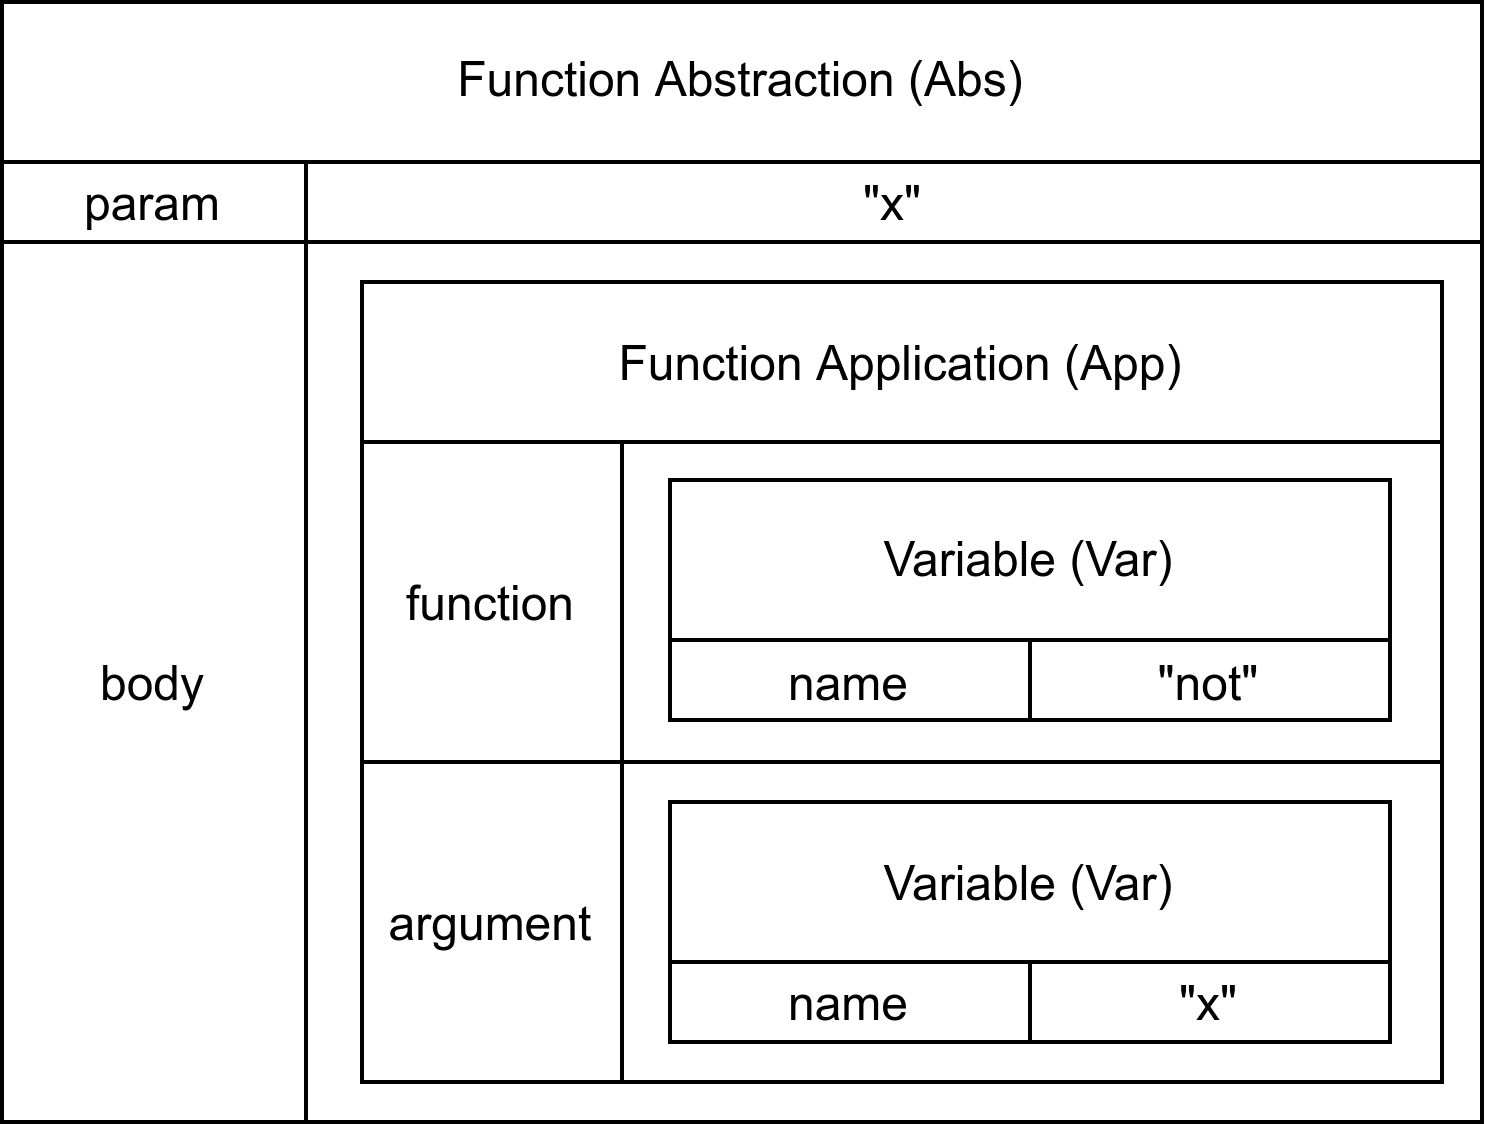
\includegraphics[width=1.000\linewidth]{images/image18.png}
  \caption{An automated test for the web application, which ensures the front-end integrates with the inference algorithm to display the correct result.}
\end{figure}

Git was used for version control, as it is robust, well-used and familiar to me. Version control allows rolling back to previous working versions of the software if necessary, and acts as a change log of how the project has evolved. While this was not used, being able to do so allowed making potentially drastic changes with confidence, which could not have been done without version control. Git also makes diffing versions of the code and reports easy, so my supervisor could easily determine what has changed since last view.

GitHub was used for git hosting, which allowed me to easily sync changes between machines, and allowed sharing the code with my supervisor easily. GitHub also acted as an external backup of the code. This ensures my work would not be lost if my personal computer was. However, a bad force push could theoretically cause data loss, so at major milestones I stored snapshots of the code on Google Cloud Platform (avoiding AWS and Azure to maximise resiliency, as GitHub runs on a combination of the two).

In my project specification, GitHub was considered for project, issue and pull request management. However after evaluating the project needs this was found to be unnecessary. As a single developer I am able to understand the overall structure of the code having written all of it, and a simple notepad has sufficed for task tracking.

GitHub Actions provided continuous integration (CI). At each commit to the GitHub repository, the changes would be built and automatically tested. If the CI failed, an automated email would be sent giving build and test failure visibility. If the CI passed, the web application was automatically re-deployed to be kept up to date with any changes. In this way, my supervisor and other users are always able to easily try out the latest version of the application.

Most of the system is written in TypeScript, a programming language developed by Microsoft, for reasons explained in the design chapter. The VS Code editor was used to write code, as it is the most popular editor for TypeScript, with strong language features such as autocomplete and automatic suggestions from an in-built linting tool. Additionally, I have used VS Code in the past, and it is multi-purpose, allowing me to also edit the LaTeX sources for the project specification and reports.

Draft reports have been written in Google Docs, as it is easy to use, version-controlled and offers good reviewing features. At major milestones this is synced with the git repository, so is included in the git backup on GitHub and Google Cloud Platform. For more control over typesetting, the purpose-built tool gdoc2latex\footnote{\href{https://github.com/domdomegg/gdoc2latex}{https://github.com/domdomegg/gdoc2latex}} was developed to convert a Google Docs document to a LaTeX document. GitHub actions automatically uses this tool to keep the Google Docs and LaTeX versions in sync within the repository, as well as automatically build the sources to a PDF. It was found through performance comparisons that to run the LaTeX commands it was significantly faster to reinstall them to the runner for each CI run rather than use a pre-built Docker container.

\section{Communication and meetings}\label{id:h.k8ippxnoat7q}

Due to the ongoing COVID-19 pandemic, all communication and meetings took place online. Throughout the project’s lifetime the UK has gone through several changes in restrictions, including the Tier 3 rules applied to Coventry and the national lockdown. However, this has not significantly disrupted the project as appropriate risk-mitigation strategies were in place, with plans to continue meeting online through Microsoft Teams and Slack working well.

Weekly supervisor meetings during term-time and the Easter holidays kept my supervisor updated on the project progress and helped to quickly resolve all issues encountered. The beginning of the project required the most guidance as understanding existing resources on type systems was challenging. It is of course hoped that this teaching tool will make understanding these complex topics I initially struggled with significantly easier.

\chapter{Conclusions}\label{id:h.90axtam6qk9n}

Static typing eliminates runtime type errors, acts as a form of documentation, and supports IDEs in increasing developer productivity. Specifying types manually is time-consuming, so many languages implement type inference which allows types to be determined automatically. Understanding this type inference can help programmers debug their code and use types more effectively in their programs.

In this project we present a teaching tool for type inference, that visualises the steps common type inference algorithms \W, \W’ and \M\ take on the Hindley-Milner system. Its design strives to overcome issues found in exploring existing type inference resources, ensuring the tool is a useful and long-lasting teaching resource.

The tool is composed of several TypeScript modules that support a React web application running entirely in the browser. The type inference algorithms are implemented following their formal definitions, using helper functions from a language core. Each module is extensively tested to ensure correctness, which allowed for the several significant refactorings that took place to reach the final code's structure.

The project's success as a teaching tool is evaluated by examining responses to a questionnaire and exploring analytics data. This questionnaire’s open-ended responses show users think that “the step by step breakdown is really well explained”, and the before and after tests show that using the tool improves students' understanding of type and type inference, no matter the students' previous experience. Analytics data confirms users are able to use the tool, and suggests users are able to interpret its results to debug type-errors.

The project was also successful in achieving all of its objectives and completing all potential extensions set out in the original specification. However, it could be extended further to add the additional features requested by users through the questionnaire. These include supporting performing inference in custom contexts, and introducing a tutorial page which explains the Hinldey-Milner type system to users more gradually. In addition to these suggestions, as the libraries work independently of the tool's web application, completely different applications could be built relating to type inference allowing for different perspectives with perhaps a more quiz-like gamified experience.

\chapter*{Acknowledgements}\label{id:h.xqaef57orpsv}

This project would not have been possible without the support of my supervisor, Michael Gale. His feedback on drafts and answers to my many questions on type inference have been invaluable throughout.

The detailed evaluation of the tool is a result of the many kind volunteers who offered to try the application and complete the questionnaire. Thanks are due to all those who used the tool, and in particular to any who provided feedback on how it could be improved.

This document was typeset using a derivative of the CS310 starter pack\footnote{\href{https://github.com/mbg/cs310}{https://github.com/mbg/cs310}} by Michael Gale, licensed under CC BY 4.0. Parts of the introduction and project management sections of this report are adapted from my project specification and progress report.

\bibliographystyle{./plainnat}
\bibliography{./index}

\end{document}